\documentclass[twoside]{book}

% Packages required by doxygen
\usepackage{fixltx2e}
\usepackage{calc}
\usepackage{doxygen}
\usepackage[export]{adjustbox} % also loads graphicx
\usepackage{graphicx}
\usepackage[utf8]{inputenc}
\usepackage{makeidx}
\usepackage{multicol}
\usepackage{multirow}
\PassOptionsToPackage{warn}{textcomp}
\usepackage{textcomp}
\usepackage[nointegrals]{wasysym}
\usepackage[table]{xcolor}

% NLS support packages
\usepackage[spanish]{babel}
% Font selection
\usepackage[T1]{fontenc}
\usepackage[scaled=.90]{helvet}
\usepackage{courier}
\usepackage{amssymb}
\usepackage{sectsty}
\renewcommand{\familydefault}{\sfdefault}
\allsectionsfont{%
  \fontseries{bc}\selectfont%
  \color{darkgray}%
}
\renewcommand{\DoxyLabelFont}{%
  \fontseries{bc}\selectfont%
  \color{darkgray}%
}
\newcommand{\+}{\discretionary{\mbox{\scriptsize$\hookleftarrow$}}{}{}}

% Page & text layout
\usepackage{geometry}
\geometry{%
  a4paper,%
  top=2.5cm,%
  bottom=2.5cm,%
  left=2.5cm,%
  right=2.5cm%
}
\tolerance=750
\hfuzz=15pt
\hbadness=750
\setlength{\emergencystretch}{15pt}
\setlength{\parindent}{0cm}
\setlength{\parskip}{3ex plus 2ex minus 2ex}
\makeatletter
\renewcommand{\paragraph}{%
  \@startsection{paragraph}{4}{0ex}{-1.0ex}{1.0ex}{%
    \normalfont\normalsize\bfseries\SS@parafont%
  }%
}
\renewcommand{\subparagraph}{%
  \@startsection{subparagraph}{5}{0ex}{-1.0ex}{1.0ex}{%
    \normalfont\normalsize\bfseries\SS@subparafont%
  }%
}
\makeatother

% Headers & footers
\usepackage{fancyhdr}
\pagestyle{fancyplain}
\fancyhead[LE]{\fancyplain{}{\bfseries\thepage}}
\fancyhead[CE]{\fancyplain{}{}}
\fancyhead[RE]{\fancyplain{}{\bfseries\leftmark}}
\fancyhead[LO]{\fancyplain{}{\bfseries\rightmark}}
\fancyhead[CO]{\fancyplain{}{}}
\fancyhead[RO]{\fancyplain{}{\bfseries\thepage}}
\fancyfoot[LE]{\fancyplain{}{}}
\fancyfoot[CE]{\fancyplain{}{}}
\fancyfoot[RE]{\fancyplain{}{\bfseries\scriptsize Generado por Doxygen }}
\fancyfoot[LO]{\fancyplain{}{\bfseries\scriptsize Generado por Doxygen }}
\fancyfoot[CO]{\fancyplain{}{}}
\fancyfoot[RO]{\fancyplain{}{}}
\renewcommand{\footrulewidth}{0.4pt}
\renewcommand{\chaptermark}[1]{%
  \markboth{#1}{}%
}
\renewcommand{\sectionmark}[1]{%
  \markright{\thesection\ #1}%
}

% Indices & bibliography
\usepackage{natbib}
\usepackage[titles]{tocloft}
\setcounter{tocdepth}{3}
\setcounter{secnumdepth}{5}
\makeindex

% Hyperlinks (required, but should be loaded last)
\usepackage{ifpdf}
\ifpdf
  \usepackage[pdftex,pagebackref=true]{hyperref}
\else
  \usepackage[ps2pdf,pagebackref=true]{hyperref}
\fi
\hypersetup{%
  colorlinks=true,%
  linkcolor=blue,%
  citecolor=blue,%
  unicode%
}

% Custom commands
\newcommand{\clearemptydoublepage}{%
  \newpage{\pagestyle{empty}\cleardoublepage}%
}

\usepackage{caption}
\captionsetup{labelsep=space,justification=centering,font={bf},singlelinecheck=off,skip=4pt,position=top}

%===== C O N T E N T S =====

\begin{document}

% Titlepage & ToC
\hypersetup{pageanchor=false,
             bookmarksnumbered=true,
             pdfencoding=unicode
            }
\pagenumbering{alph}
\begin{titlepage}
\vspace*{7cm}
\begin{center}%
{\Large Programa principal E\+V\+A\+L\+U\+A\+T\+OR\+: plataforma de gestión de problemas y cursos de programación. \\[1ex]\large version 1 12-\/abr-\/2021 }\\
\vspace*{1cm}
{\large Generado por Doxygen 1.8.14}\\
\end{center}
\end{titlepage}
\clearemptydoublepage
\pagenumbering{roman}
\tableofcontents
\clearemptydoublepage
\pagenumbering{arabic}
\hypersetup{pageanchor=true}

%--- Begin generated contents ---
\chapter{Programa usando diseño modular\+: \char`\"{}\+Evaluator\char`\"{}.}
\label{index}\hypertarget{index}{}En esta práctica se evalua tanto la especificación como la implementación de una plataforma llamada {\itshape Evaluator} que ofrece un menú de comandos que permiten evaluar ejercicios de programación. En esta práctica se introducen las clases {\itshape \mbox{\hyperlink{class_user_set}{User\+Set}}}, {\itshape \mbox{\hyperlink{class_user}{User}}}, {\itshape \mbox{\hyperlink{class_course_set}{Course\+Set}}}, {\itshape \mbox{\hyperlink{class_course}{Course}}}, {\itshape \mbox{\hyperlink{class_sesion_set}{Sesion\+Set}}}, {\itshape \mbox{\hyperlink{class_sesion}{Sesion}}}, {\itshape \mbox{\hyperlink{class_problem_set}{Problem\+Set}}} y {\itshape \mbox{\hyperlink{class_problem}{Problem}}} 
\chapter{Índice de clases}
\section{Lista de clases}
Lista de las clases, estructuras, uniones e interfaces con una breve descripción\+:\begin{DoxyCompactList}
\item\contentsline{section}{\mbox{\hyperlink{class_bin_tree}{Bin\+Tree$<$ T $>$}} }{\pageref{class_bin_tree}}{}
\item\contentsline{section}{\mbox{\hyperlink{class_course}{Course}} \\*Representa un curso con el numero de usuarios con el curso completado, el numero de usuarios inscritos actualmente en el curso y el número de sesiones que lo forman con su identificador (en el orden que se leyeron al introducirlas en el curso) }{\pageref{class_course}}{}
\item\contentsline{section}{\mbox{\hyperlink{class_course_set}{Course\+Set}} \\*Representa un conjunto de cursos ordenados crecientemente por id }{\pageref{class_course_set}}{}
\item\contentsline{section}{\mbox{\hyperlink{class_problem}{Problem}} \\*Representa un problema con atributos identificador = id, envios totales = t , envios exito = e y ratio = r = (t+1)/(e+1) }{\pageref{class_problem}}{}
\item\contentsline{section}{\mbox{\hyperlink{class_problem_set}{Problem\+Set}} \\*Representa un conjunto de problemas ordenados crecientemente por id }{\pageref{class_problem_set}}{}
\item\contentsline{section}{\mbox{\hyperlink{class_sesion}{Sesion}} \\*Representa una sesion con el numero de problemas en esta contenidos en un \mbox{\hyperlink{class_bin_tree}{Bin\+Tree}} }{\pageref{class_sesion}}{}
\item\contentsline{section}{\mbox{\hyperlink{class_sesion_set}{Sesion\+Set}} \\*Representa un conjunto de sesiones ordenados crecientemente por id }{\pageref{class_sesion_set}}{}
\item\contentsline{section}{\mbox{\hyperlink{class_user}{User}} \\*Representa un usuario con el numero de envios\+\_\+totales que ha realizado, el número de problemas resueltos, el número de problemas intentados en total, el curso en el qual está inscrito (si lo está) y dos \mbox{\hyperlink{class_problem_set}{Problem\+Set}} con los problemas\+\_\+resueltos y los problemas\+\_\+enviables respectivamente }{\pageref{class_user}}{}
\item\contentsline{section}{\mbox{\hyperlink{class_user_set}{User\+Set}} \\*Representa un conjunto de usuario ordenados crecientemente por id }{\pageref{class_user_set}}{}
\end{DoxyCompactList}

\chapter{Indice de archivos}
\section{Lista de archivos}
Lista de todos los archivos con descripciones breves\+:\begin{DoxyCompactList}
\item\contentsline{section}{\mbox{\hyperlink{_bin_tree_8hh}{Bin\+Tree.\+hh}} }{\pageref{_bin_tree_8hh}}{}
\item\contentsline{section}{\mbox{\hyperlink{_course_8hh}{Course.\+hh}} \\*Especificación de la clase Curso }{\pageref{_course_8hh}}{}
\item\contentsline{section}{\mbox{\hyperlink{_course_set_8hh}{Course\+Set.\+hh}} \\*Especificación de la clase Curso }{\pageref{_course_set_8hh}}{}
\item\contentsline{section}{\mbox{\hyperlink{main_8cc}{main.\+cc}} \\*Programa principal E\+V\+A\+L\+U\+A\+T\+OR\+: plataforma de gestión de problemas y cursos de programación }{\pageref{main_8cc}}{}
\item\contentsline{section}{\mbox{\hyperlink{_problem_8hh}{Problem.\+hh}} \\*Especificación de la clase \mbox{\hyperlink{class_problem}{Problem}} }{\pageref{_problem_8hh}}{}
\item\contentsline{section}{\mbox{\hyperlink{_problem_set_8hh}{Problem\+Set.\+hh}} \\*Especificación de la clase \mbox{\hyperlink{class_problem_set}{Problem\+Set}} }{\pageref{_problem_set_8hh}}{}
\item\contentsline{section}{\mbox{\hyperlink{_sesion_8hh}{Sesion.\+hh}} \\*Especificación de la clase \mbox{\hyperlink{class_sesion}{Sesion}} }{\pageref{_sesion_8hh}}{}
\item\contentsline{section}{\mbox{\hyperlink{_sesion_set_8hh}{Sesion\+Set.\+hh}} \\*Especificación de la clase \mbox{\hyperlink{class_sesion_set}{Sesion\+Set}} }{\pageref{_sesion_set_8hh}}{}
\item\contentsline{section}{\mbox{\hyperlink{_user_8hh}{User.\+hh}} \\*Especificación de la clase Usuario }{\pageref{_user_8hh}}{}
\item\contentsline{section}{\mbox{\hyperlink{_user_set_8hh}{User\+Set.\+hh}} \\*Especificación de la clase \mbox{\hyperlink{class_user_set}{User\+Set}} }{\pageref{_user_set_8hh}}{}
\end{DoxyCompactList}

\chapter{Documentación de las clases}
\hypertarget{class_bin_tree}{}\section{Referencia de la plantilla de la Clase Bin\+Tree$<$ T $>$}
\label{class_bin_tree}\index{Bin\+Tree$<$ T $>$@{Bin\+Tree$<$ T $>$}}
\subsection*{Métodos públicos}
\begin{DoxyCompactItemize}
\item 
\mbox{\hyperlink{class_bin_tree_a47eef22d29cd023449d97c073c08e5b6}{Bin\+Tree}} ()
\item 
\mbox{\hyperlink{class_bin_tree_a1ab686e0bcf990093ff91fe71744c1a4}{Bin\+Tree}} (const T \&x)
\item 
\mbox{\hyperlink{class_bin_tree_adb7eeff76d08130c943b36af215eb521}{Bin\+Tree}} (const T \&x, const \mbox{\hyperlink{class_bin_tree}{Bin\+Tree}} \&\mbox{\hyperlink{class_bin_tree_a82108db4c1b08d1f111027788c196d4e}{left}}, const \mbox{\hyperlink{class_bin_tree}{Bin\+Tree}} \&\mbox{\hyperlink{class_bin_tree_aff8e96651b27284c329667b5ad3e4d0b}{right}})
\item 
bool \mbox{\hyperlink{class_bin_tree_a74cda259ba5c25b8ee38ed4dc33e4fad}{empty}} () const
\item 
\mbox{\hyperlink{class_bin_tree}{Bin\+Tree}} \mbox{\hyperlink{class_bin_tree_a82108db4c1b08d1f111027788c196d4e}{left}} () const
\item 
\mbox{\hyperlink{class_bin_tree}{Bin\+Tree}} \mbox{\hyperlink{class_bin_tree_aff8e96651b27284c329667b5ad3e4d0b}{right}} () const
\item 
const T \& \mbox{\hyperlink{class_bin_tree_a734e785b089c87b49187ee7c58edf5f3}{value}} () const
\end{DoxyCompactItemize}


\subsection{Descripción detallada}
\subsubsection*{template$<$typename T$>$\newline
class Bin\+Tree$<$ T $>$}



Definición en la línea 15 del archivo Bin\+Tree.\+hh.



\subsection{Documentación del constructor y destructor}
\mbox{\Hypertarget{class_bin_tree_a47eef22d29cd023449d97c073c08e5b6}\label{class_bin_tree_a47eef22d29cd023449d97c073c08e5b6}} 
\index{Bin\+Tree@{Bin\+Tree}!Bin\+Tree@{Bin\+Tree}}
\index{Bin\+Tree@{Bin\+Tree}!Bin\+Tree@{Bin\+Tree}}
\subsubsection{\texorpdfstring{Bin\+Tree()}{BinTree()}\hspace{0.1cm}{\footnotesize\ttfamily [1/3]}}
{\footnotesize\ttfamily template$<$typename T$>$ \\
\mbox{\hyperlink{class_bin_tree}{Bin\+Tree}}$<$ T $>$\+::\mbox{\hyperlink{class_bin_tree}{Bin\+Tree}} (\begin{DoxyParamCaption}{ }\end{DoxyParamCaption})}



Definición en la línea 44 del archivo Bin\+Tree.\+hh.


\begin{DoxyCode}
45     :   p(\textcolor{keyword}{nullptr})
46     \{   \}
\end{DoxyCode}
\mbox{\Hypertarget{class_bin_tree_a1ab686e0bcf990093ff91fe71744c1a4}\label{class_bin_tree_a1ab686e0bcf990093ff91fe71744c1a4}} 
\index{Bin\+Tree@{Bin\+Tree}!Bin\+Tree@{Bin\+Tree}}
\index{Bin\+Tree@{Bin\+Tree}!Bin\+Tree@{Bin\+Tree}}
\subsubsection{\texorpdfstring{Bin\+Tree()}{BinTree()}\hspace{0.1cm}{\footnotesize\ttfamily [2/3]}}
{\footnotesize\ttfamily template$<$typename T$>$ \\
\mbox{\hyperlink{class_bin_tree}{Bin\+Tree}}$<$ T $>$\+::\mbox{\hyperlink{class_bin_tree}{Bin\+Tree}} (\begin{DoxyParamCaption}\item[{const T \&}]{x }\end{DoxyParamCaption})\hspace{0.3cm}{\ttfamily [explicit]}}



Definición en la línea 49 del archivo Bin\+Tree.\+hh.


\begin{DoxyCode}
49                                   \{
50         p = make\_shared<Node>(x, \textcolor{keyword}{nullptr}, \textcolor{keyword}{nullptr});
51     \}
\end{DoxyCode}
\mbox{\Hypertarget{class_bin_tree_adb7eeff76d08130c943b36af215eb521}\label{class_bin_tree_adb7eeff76d08130c943b36af215eb521}} 
\index{Bin\+Tree@{Bin\+Tree}!Bin\+Tree@{Bin\+Tree}}
\index{Bin\+Tree@{Bin\+Tree}!Bin\+Tree@{Bin\+Tree}}
\subsubsection{\texorpdfstring{Bin\+Tree()}{BinTree()}\hspace{0.1cm}{\footnotesize\ttfamily [3/3]}}
{\footnotesize\ttfamily template$<$typename T$>$ \\
\mbox{\hyperlink{class_bin_tree}{Bin\+Tree}}$<$ T $>$\+::\mbox{\hyperlink{class_bin_tree}{Bin\+Tree}} (\begin{DoxyParamCaption}\item[{const T \&}]{x,  }\item[{const \mbox{\hyperlink{class_bin_tree}{Bin\+Tree}}$<$ T $>$ \&}]{left,  }\item[{const \mbox{\hyperlink{class_bin_tree}{Bin\+Tree}}$<$ T $>$ \&}]{right }\end{DoxyParamCaption})\hspace{0.3cm}{\ttfamily [explicit]}}



Definición en la línea 54 del archivo Bin\+Tree.\+hh.


\begin{DoxyCode}
54                                                                              \{
55         p = make\_shared<Node>(x, \mbox{\hyperlink{class_bin_tree_a82108db4c1b08d1f111027788c196d4e}{left}}.p, \mbox{\hyperlink{class_bin_tree_aff8e96651b27284c329667b5ad3e4d0b}{right}}.p);
56     \}
\end{DoxyCode}


\subsection{Documentación de las funciones miembro}
\mbox{\Hypertarget{class_bin_tree_a74cda259ba5c25b8ee38ed4dc33e4fad}\label{class_bin_tree_a74cda259ba5c25b8ee38ed4dc33e4fad}} 
\index{Bin\+Tree@{Bin\+Tree}!empty@{empty}}
\index{empty@{empty}!Bin\+Tree@{Bin\+Tree}}
\subsubsection{\texorpdfstring{empty()}{empty()}}
{\footnotesize\ttfamily template$<$typename T$>$ \\
bool \mbox{\hyperlink{class_bin_tree}{Bin\+Tree}}$<$ T $>$\+::empty (\begin{DoxyParamCaption}{ }\end{DoxyParamCaption}) const}



Definición en la línea 59 del archivo Bin\+Tree.\+hh.


\begin{DoxyCode}
59                         \{
60         \textcolor{keywordflow}{return} not p;
61     \}
\end{DoxyCode}
\mbox{\Hypertarget{class_bin_tree_a82108db4c1b08d1f111027788c196d4e}\label{class_bin_tree_a82108db4c1b08d1f111027788c196d4e}} 
\index{Bin\+Tree@{Bin\+Tree}!left@{left}}
\index{left@{left}!Bin\+Tree@{Bin\+Tree}}
\subsubsection{\texorpdfstring{left()}{left()}}
{\footnotesize\ttfamily template$<$typename T$>$ \\
\mbox{\hyperlink{class_bin_tree}{Bin\+Tree}} \mbox{\hyperlink{class_bin_tree}{Bin\+Tree}}$<$ T $>$\+::left (\begin{DoxyParamCaption}{ }\end{DoxyParamCaption}) const}



Definición en la línea 64 del archivo Bin\+Tree.\+hh.


\begin{DoxyCode}
64                           \{
65         assert(not \mbox{\hyperlink{class_bin_tree_a74cda259ba5c25b8ee38ed4dc33e4fad}{empty}}());
66         \textcolor{keywordflow}{return} \mbox{\hyperlink{class_bin_tree_a47eef22d29cd023449d97c073c08e5b6}{BinTree}}(p->left);
67     \}
\end{DoxyCode}
\mbox{\Hypertarget{class_bin_tree_aff8e96651b27284c329667b5ad3e4d0b}\label{class_bin_tree_aff8e96651b27284c329667b5ad3e4d0b}} 
\index{Bin\+Tree@{Bin\+Tree}!right@{right}}
\index{right@{right}!Bin\+Tree@{Bin\+Tree}}
\subsubsection{\texorpdfstring{right()}{right()}}
{\footnotesize\ttfamily template$<$typename T$>$ \\
\mbox{\hyperlink{class_bin_tree}{Bin\+Tree}} \mbox{\hyperlink{class_bin_tree}{Bin\+Tree}}$<$ T $>$\+::right (\begin{DoxyParamCaption}{ }\end{DoxyParamCaption}) const}



Definición en la línea 70 del archivo Bin\+Tree.\+hh.


\begin{DoxyCode}
70                            \{
71         assert(not \mbox{\hyperlink{class_bin_tree_a74cda259ba5c25b8ee38ed4dc33e4fad}{empty}}());
72         \textcolor{keywordflow}{return} \mbox{\hyperlink{class_bin_tree_a47eef22d29cd023449d97c073c08e5b6}{BinTree}}(p->right);
73     \}
\end{DoxyCode}
\mbox{\Hypertarget{class_bin_tree_a734e785b089c87b49187ee7c58edf5f3}\label{class_bin_tree_a734e785b089c87b49187ee7c58edf5f3}} 
\index{Bin\+Tree@{Bin\+Tree}!value@{value}}
\index{value@{value}!Bin\+Tree@{Bin\+Tree}}
\subsubsection{\texorpdfstring{value()}{value()}}
{\footnotesize\ttfamily template$<$typename T$>$ \\
const T\& \mbox{\hyperlink{class_bin_tree}{Bin\+Tree}}$<$ T $>$\+::value (\begin{DoxyParamCaption}{ }\end{DoxyParamCaption}) const}



Definición en la línea 76 del archivo Bin\+Tree.\+hh.


\begin{DoxyCode}
76                             \{
77         assert(not \mbox{\hyperlink{class_bin_tree_a74cda259ba5c25b8ee38ed4dc33e4fad}{empty}}());
78         \textcolor{keywordflow}{return} p->x;
79     \}
\end{DoxyCode}


La documentación para esta clase fue generada a partir del siguiente fichero\+:\begin{DoxyCompactItemize}
\item 
\mbox{\hyperlink{_bin_tree_8hh}{Bin\+Tree.\+hh}}\end{DoxyCompactItemize}

\hypertarget{class_course}{}\section{Referencia de la Clase Course}
\label{class_course}\index{Course@{Course}}


Representa un curso con el numero de usuarios con el curso completado, el numero de usuarios inscritos actualmente en el curso y el número de sesiones que lo forman con su identificador (en el orden que se leyeron al introducirlas en el curso).  


\subsection*{Métodos públicos}
\begin{DoxyCompactItemize}
\item 
\mbox{\hyperlink{class_course_a6b959ccf15d9ceed9e9c14a701561982}{Course}} ()
\begin{DoxyCompactList}\small\item\em Creadora por defecto. \end{DoxyCompactList}\item 
int \mbox{\hyperlink{class_course_ad17501c45b744c632235c05365f05f1d}{Get\+Num\+Users\+Done}} () const
\begin{DoxyCompactList}\small\item\em Consultora del número de usuarios completados. \end{DoxyCompactList}\item 
int \mbox{\hyperlink{class_course_a3ce2bc364698f6857385d7bb0ea82812}{Get\+Num\+Users\+In}} () const
\begin{DoxyCompactList}\small\item\em Consultora del número de usuarios inscritos. \end{DoxyCompactList}\item 
void \mbox{\hyperlink{class_course_a56a7f6bfd9dcd415c35246b2dc4afddb}{Get\+Sesion}} (string id\+\_\+problema) const
\begin{DoxyCompactList}\small\item\em Consultora de la sesion que contiene el problema id\+\_\+problema en el parametro implícito. \end{DoxyCompactList}\item 
void \mbox{\hyperlink{class_course_aa44f6ece5bc630400d9e7edff41680c0}{Increase\+Num\+Users\+Done}} ()
\begin{DoxyCompactList}\small\item\em Modificadora del número de usuarios completados. \end{DoxyCompactList}\item 
void \mbox{\hyperlink{class_course_ab1bf31a23895b7ece77ab0c74a4de321}{Increase\+Num\+Users\+In}} ()
\begin{DoxyCompactList}\small\item\em Modificadora del número de usuarios inscritos. \end{DoxyCompactList}\item 
void \mbox{\hyperlink{class_course_ab23d9a5201da47a27d9b307a5889ca23}{Decrease\+Num\+Users\+In}} ()
\begin{DoxyCompactList}\small\item\em Modificadora del número de usuarios inscritos. \end{DoxyCompactList}\item 
void \mbox{\hyperlink{class_course_ae6becc4684a1ae379b9e26b4b50d8d23}{Print\+Course}} () const
\begin{DoxyCompactList}\small\item\em Operación de escritura. \end{DoxyCompactList}\end{DoxyCompactItemize}


\subsection{Descripción detallada}
Representa un curso con el numero de usuarios con el curso completado, el numero de usuarios inscritos actualmente en el curso y el número de sesiones que lo forman con su identificador (en el orden que se leyeron al introducirlas en el curso). 

Definición en la línea 19 del archivo Course.\+hh.



\subsection{Documentación del constructor y destructor}
\mbox{\Hypertarget{class_course_a6b959ccf15d9ceed9e9c14a701561982}\label{class_course_a6b959ccf15d9ceed9e9c14a701561982}} 
\index{Course@{Course}!Course@{Course}}
\index{Course@{Course}!Course@{Course}}
\subsubsection{\texorpdfstring{Course()}{Course()}}
{\footnotesize\ttfamily Course\+::\+Course (\begin{DoxyParamCaption}{ }\end{DoxyParamCaption})}



Creadora por defecto. 

\begin{DoxyPrecond}{Precondición}
{\itshape Cierto.} 
\end{DoxyPrecond}
\begin{DoxyPostcond}{Postcondición}
El resultado es un curso sin id, num\+\_\+usuarios\+\_\+inscritos = 0, num\+\_\+usuarios\+\_\+completado = 0 y la lista de problemas vacia. 
\end{DoxyPostcond}


\subsection{Documentación de las funciones miembro}
\mbox{\Hypertarget{class_course_ad17501c45b744c632235c05365f05f1d}\label{class_course_ad17501c45b744c632235c05365f05f1d}} 
\index{Course@{Course}!Get\+Num\+Users\+Done@{Get\+Num\+Users\+Done}}
\index{Get\+Num\+Users\+Done@{Get\+Num\+Users\+Done}!Course@{Course}}
\subsubsection{\texorpdfstring{Get\+Num\+Users\+Done()}{GetNumUsersDone()}}
{\footnotesize\ttfamily int Course\+::\+Get\+Num\+Users\+Done (\begin{DoxyParamCaption}{ }\end{DoxyParamCaption}) const}



Consultora del número de usuarios completados. 

\begin{DoxyPrecond}{Precondición}
{\itshape Cierto.} 
\end{DoxyPrecond}
\begin{DoxyPostcond}{Postcondición}
El resultado es el número de usuarios que han completado el parámetro implícito. 
\end{DoxyPostcond}
\mbox{\Hypertarget{class_course_a3ce2bc364698f6857385d7bb0ea82812}\label{class_course_a3ce2bc364698f6857385d7bb0ea82812}} 
\index{Course@{Course}!Get\+Num\+Users\+In@{Get\+Num\+Users\+In}}
\index{Get\+Num\+Users\+In@{Get\+Num\+Users\+In}!Course@{Course}}
\subsubsection{\texorpdfstring{Get\+Num\+Users\+In()}{GetNumUsersIn()}}
{\footnotesize\ttfamily int Course\+::\+Get\+Num\+Users\+In (\begin{DoxyParamCaption}{ }\end{DoxyParamCaption}) const}



Consultora del número de usuarios inscritos. 

\begin{DoxyPrecond}{Precondición}
{\itshape Cierto.} 
\end{DoxyPrecond}
\begin{DoxyPostcond}{Postcondición}
El resultado es el número de usuarios inscritos (actualmente) en el parámetro implícito. 
\end{DoxyPostcond}
\mbox{\Hypertarget{class_course_a56a7f6bfd9dcd415c35246b2dc4afddb}\label{class_course_a56a7f6bfd9dcd415c35246b2dc4afddb}} 
\index{Course@{Course}!Get\+Sesion@{Get\+Sesion}}
\index{Get\+Sesion@{Get\+Sesion}!Course@{Course}}
\subsubsection{\texorpdfstring{Get\+Sesion()}{GetSesion()}}
{\footnotesize\ttfamily void Course\+::\+Get\+Sesion (\begin{DoxyParamCaption}\item[{string}]{id\+\_\+problema }\end{DoxyParamCaption}) const}



Consultora de la sesion que contiene el problema id\+\_\+problema en el parametro implícito. 

\begin{DoxyPrecond}{Precondición}
El problema id\+\_\+problema no es vacío. 
\end{DoxyPrecond}
\begin{DoxyPostcond}{Postcondición}
Devuelve la sesión en la que se encuentra el problema con id = id\+\_\+problema en el parametro implícito. 
\end{DoxyPostcond}
\mbox{\Hypertarget{class_course_aa44f6ece5bc630400d9e7edff41680c0}\label{class_course_aa44f6ece5bc630400d9e7edff41680c0}} 
\index{Course@{Course}!Increase\+Num\+Users\+Done@{Increase\+Num\+Users\+Done}}
\index{Increase\+Num\+Users\+Done@{Increase\+Num\+Users\+Done}!Course@{Course}}
\subsubsection{\texorpdfstring{Increase\+Num\+Users\+Done()}{IncreaseNumUsersDone()}}
{\footnotesize\ttfamily void Course\+::\+Increase\+Num\+Users\+Done (\begin{DoxyParamCaption}{ }\end{DoxyParamCaption})}



Modificadora del número de usuarios completados. 

\begin{DoxyPrecond}{Precondición}
{\itshape Cierto.} 
\end{DoxyPrecond}
\begin{DoxyPostcond}{Postcondición}
Se incrementará el número de usuarios con el parámetro ímplicito completado. 
\end{DoxyPostcond}
\mbox{\Hypertarget{class_course_ab1bf31a23895b7ece77ab0c74a4de321}\label{class_course_ab1bf31a23895b7ece77ab0c74a4de321}} 
\index{Course@{Course}!Increase\+Num\+Users\+In@{Increase\+Num\+Users\+In}}
\index{Increase\+Num\+Users\+In@{Increase\+Num\+Users\+In}!Course@{Course}}
\subsubsection{\texorpdfstring{Increase\+Num\+Users\+In()}{IncreaseNumUsersIn()}}
{\footnotesize\ttfamily void Course\+::\+Increase\+Num\+Users\+In (\begin{DoxyParamCaption}{ }\end{DoxyParamCaption})}



Modificadora del número de usuarios inscritos. 

\begin{DoxyPrecond}{Precondición}
{\itshape Cierto.} 
\end{DoxyPrecond}
\begin{DoxyPostcond}{Postcondición}
Se incrementará el número de usuarios inscritos (actualmente) en el parámetro implícito. 
\end{DoxyPostcond}
\mbox{\Hypertarget{class_course_ab23d9a5201da47a27d9b307a5889ca23}\label{class_course_ab23d9a5201da47a27d9b307a5889ca23}} 
\index{Course@{Course}!Decrease\+Num\+Users\+In@{Decrease\+Num\+Users\+In}}
\index{Decrease\+Num\+Users\+In@{Decrease\+Num\+Users\+In}!Course@{Course}}
\subsubsection{\texorpdfstring{Decrease\+Num\+Users\+In()}{DecreaseNumUsersIn()}}
{\footnotesize\ttfamily void Course\+::\+Decrease\+Num\+Users\+In (\begin{DoxyParamCaption}{ }\end{DoxyParamCaption})}



Modificadora del número de usuarios inscritos. 

\begin{DoxyPrecond}{Precondición}
{\itshape Cierto.} 
\end{DoxyPrecond}
\begin{DoxyPostcond}{Postcondición}
Se decrementará el número de usuarios inscritos (actualmente) en el parámetro implícito. 
\end{DoxyPostcond}
\mbox{\Hypertarget{class_course_ae6becc4684a1ae379b9e26b4b50d8d23}\label{class_course_ae6becc4684a1ae379b9e26b4b50d8d23}} 
\index{Course@{Course}!Print\+Course@{Print\+Course}}
\index{Print\+Course@{Print\+Course}!Course@{Course}}
\subsubsection{\texorpdfstring{Print\+Course()}{PrintCourse()}}
{\footnotesize\ttfamily void Course\+::\+Print\+Course (\begin{DoxyParamCaption}{ }\end{DoxyParamCaption}) const}



Operación de escritura. 

\begin{DoxyPrecond}{Precondición}
{\itshape Cierto.} 
\end{DoxyPrecond}
\begin{DoxyPostcond}{Postcondición}
Se han escrito los atributos (num\+\_\+usuarios\+\_\+completados, num\+\_\+usuarios\+\_\+inscritos, num\+\_\+sesiones + id\+\_\+sesiones de estas en el orden que se creó el curso) del parametro implícito en el canal estandar de salida. 
\end{DoxyPostcond}


La documentación para esta clase fue generada a partir del siguiente fichero\+:\begin{DoxyCompactItemize}
\item 
\mbox{\hyperlink{_course_8hh}{Course.\+hh}}\end{DoxyCompactItemize}

\hypertarget{class_course_set}{}\section{Referencia de la Clase Course\+Set}
\label{class_course_set}\index{Course\+Set@{Course\+Set}}


Representa un conjunto de cursos ordenados crecientemente por id.  


\subsection*{Métodos públicos}
\begin{DoxyCompactItemize}
\item 
\mbox{\hyperlink{class_course_set_ae0b73bd2e6bda115838ba65644e015bc}{Course\+Set}} ()
\begin{DoxyCompactList}\small\item\em Creadora por defecto. \end{DoxyCompactList}\item 
int \mbox{\hyperlink{class_course_set_ac255028f38ba0b5b3ef1994e2a9a6c6f}{Size}} () const
\begin{DoxyCompactList}\small\item\em Consultora del tamaño del conjunto. \end{DoxyCompactList}\item 
bool \mbox{\hyperlink{class_course_set_a1ced9926115a2fbc8058982d148040f1}{Exist}} (int id\+\_\+curso) const
\begin{DoxyCompactList}\small\item\em Consultora de curso en \mbox{\hyperlink{class_course_set}{Course\+Set}}. \end{DoxyCompactList}\item 
bool \mbox{\hyperlink{class_course_set_a3ad118865a697fbb3e5765fc6583346e}{Exist\+Problem}} (int id\+\_\+curso, string id\+\_\+problema) const
\begin{DoxyCompactList}\small\item\em Consultora de problema en curso. \end{DoxyCompactList}\item 
int \mbox{\hyperlink{class_course_set_a46150057534a76182941f23beb2ce4cc}{Get\+Num\+Users\+Done}} (int id\+\_\+curso) const
\begin{DoxyCompactList}\small\item\em Consultora del número de usuarios completados. \end{DoxyCompactList}\item 
int \mbox{\hyperlink{class_course_set_a72b6a09b4eafce672b57abebfa9f1f55}{Get\+Num\+Users\+In}} (int id\+\_\+curso) const
\begin{DoxyCompactList}\small\item\em Consultora del número de usuarios inscritos. \end{DoxyCompactList}\item 
int \mbox{\hyperlink{class_course_set_a534fa228ab549072198b0966d159a530}{Get\+Sesion}} (int id\+\_\+curso, string id\+\_\+problema) const
\begin{DoxyCompactList}\small\item\em Consultora de la sesion que contiene el problema id\+\_\+problema en el curso id\+\_\+curso en el parámetro implícito. \end{DoxyCompactList}\item 
void \mbox{\hyperlink{class_course_set_a96eb35134feb996fdef57895074a33ff}{Update}} (int id\+\_\+curso)
\begin{DoxyCompactList}\small\item\em Modificadora del curso. \end{DoxyCompactList}\item 
int \mbox{\hyperlink{class_course_set_ae74448a3ba72c104d4f35abf41d47b0e}{Add\+One\+From\+Console}} ()
\begin{DoxyCompactList}\small\item\em Añade un curso en el conjunto. \end{DoxyCompactList}\item 
void \mbox{\hyperlink{class_course_set_ade38257bb2809e6b8a2b062796c69e53}{Increase\+Num\+Users\+Done}} (int id\+\_\+curso)
\begin{DoxyCompactList}\small\item\em Modificadora del número de usuarios completados. \end{DoxyCompactList}\item 
void \mbox{\hyperlink{class_course_set_a6a1532272c28fcb228bae6b9bde47c4e}{Increase\+Num\+Users\+In}} (int id\+\_\+curso)
\begin{DoxyCompactList}\small\item\em Modificadora del número de usuarios inscritos. \end{DoxyCompactList}\item 
void \mbox{\hyperlink{class_course_set_ab24913a21a3fd64d67346668dbf9159c}{Decrease\+Num\+Users\+In}} (int id\+\_\+curso)
\begin{DoxyCompactList}\small\item\em Modificadora del número de usuarios inscritos. \end{DoxyCompactList}\item 
void \mbox{\hyperlink{class_course_set_aee9d2b96c43a828049e02205736a4982}{Add\+From\+Console}} ()
\begin{DoxyCompactList}\small\item\em Operación de lectura. \end{DoxyCompactList}\item 
void \mbox{\hyperlink{class_course_set_a31726d4dcdefc4a218f9e1466fd2ef38}{List\+Course\+Set}} ()
\begin{DoxyCompactList}\small\item\em Operación de escritura. \end{DoxyCompactList}\item 
int \mbox{\hyperlink{class_course_set_aee3609cbaa62ae2be155754613d484e3}{List\+Course}} (int id\+\_\+curso)
\begin{DoxyCompactList}\small\item\em Operación de escritura. \end{DoxyCompactList}\end{DoxyCompactItemize}


\subsection{Descripción detallada}
Representa un conjunto de cursos ordenados crecientemente por id. 

Definición en la línea 21 del archivo Course\+Set.\+hh.



\subsection{Documentación del constructor y destructor}
\mbox{\Hypertarget{class_course_set_ae0b73bd2e6bda115838ba65644e015bc}\label{class_course_set_ae0b73bd2e6bda115838ba65644e015bc}} 
\index{Course\+Set@{Course\+Set}!Course\+Set@{Course\+Set}}
\index{Course\+Set@{Course\+Set}!Course\+Set@{Course\+Set}}
\subsubsection{\texorpdfstring{Course\+Set()}{CourseSet()}}
{\footnotesize\ttfamily Course\+Set\+::\+Course\+Set (\begin{DoxyParamCaption}{ }\end{DoxyParamCaption})}



Creadora por defecto. 

\begin{DoxyPrecond}{Precondición}
{\itshape Cierto.}. 
\end{DoxyPrecond}
\begin{DoxyPostcond}{Postcondición}
El resultado es un conjunto de cursos vacío. 
\end{DoxyPostcond}


\subsection{Documentación de las funciones miembro}
\mbox{\Hypertarget{class_course_set_ac255028f38ba0b5b3ef1994e2a9a6c6f}\label{class_course_set_ac255028f38ba0b5b3ef1994e2a9a6c6f}} 
\index{Course\+Set@{Course\+Set}!Size@{Size}}
\index{Size@{Size}!Course\+Set@{Course\+Set}}
\subsubsection{\texorpdfstring{Size()}{Size()}}
{\footnotesize\ttfamily int Course\+Set\+::\+Size (\begin{DoxyParamCaption}{ }\end{DoxyParamCaption}) const}



Consultora del tamaño del conjunto. 

\begin{DoxyPrecond}{Precondición}
{\itshape Cierto.} 
\end{DoxyPrecond}
\begin{DoxyPostcond}{Postcondición}
Se ha escrito por el canal estandar de salida el tamaño del parámetro implícito. 
\end{DoxyPostcond}
\mbox{\Hypertarget{class_course_set_a1ced9926115a2fbc8058982d148040f1}\label{class_course_set_a1ced9926115a2fbc8058982d148040f1}} 
\index{Course\+Set@{Course\+Set}!Exist@{Exist}}
\index{Exist@{Exist}!Course\+Set@{Course\+Set}}
\subsubsection{\texorpdfstring{Exist()}{Exist()}}
{\footnotesize\ttfamily bool Course\+Set\+::\+Exist (\begin{DoxyParamCaption}\item[{int}]{id\+\_\+curso }\end{DoxyParamCaption}) const}



Consultora de curso en \mbox{\hyperlink{class_course_set}{Course\+Set}}. 

\begin{DoxyPrecond}{Precondición}
El int id\+\_\+curso no es vacío. 
\end{DoxyPrecond}
\begin{DoxyPostcond}{Postcondición}
Devuelve un booleano conforme si existe el curso con id = id\+\_\+curso en el parámetro implícito. True si existe y false en caso contrario. 
\end{DoxyPostcond}
\mbox{\Hypertarget{class_course_set_a3ad118865a697fbb3e5765fc6583346e}\label{class_course_set_a3ad118865a697fbb3e5765fc6583346e}} 
\index{Course\+Set@{Course\+Set}!Exist\+Problem@{Exist\+Problem}}
\index{Exist\+Problem@{Exist\+Problem}!Course\+Set@{Course\+Set}}
\subsubsection{\texorpdfstring{Exist\+Problem()}{ExistProblem()}}
{\footnotesize\ttfamily bool Course\+Set\+::\+Exist\+Problem (\begin{DoxyParamCaption}\item[{int}]{id\+\_\+curso,  }\item[{string}]{id\+\_\+problema }\end{DoxyParamCaption}) const}



Consultora de problema en curso. 

\begin{DoxyPrecond}{Precondición}
El int id\+\_\+curso y el string id\+\_\+problema no són vacíos y el curso con id = id\+\_\+curso y el problema con id = id\+\_\+problem existen. 
\end{DoxyPrecond}
\begin{DoxyPostcond}{Postcondición}
Devuelve un booleano conforme si el problema con id = id\+\_\+problem existe en el curso con id = id\+\_\+curso. True si existe y false en caso contrario. 
\end{DoxyPostcond}
\mbox{\Hypertarget{class_course_set_a46150057534a76182941f23beb2ce4cc}\label{class_course_set_a46150057534a76182941f23beb2ce4cc}} 
\index{Course\+Set@{Course\+Set}!Get\+Num\+Users\+Done@{Get\+Num\+Users\+Done}}
\index{Get\+Num\+Users\+Done@{Get\+Num\+Users\+Done}!Course\+Set@{Course\+Set}}
\subsubsection{\texorpdfstring{Get\+Num\+Users\+Done()}{GetNumUsersDone()}}
{\footnotesize\ttfamily int Course\+Set\+::\+Get\+Num\+Users\+Done (\begin{DoxyParamCaption}\item[{int}]{id\+\_\+curso }\end{DoxyParamCaption}) const}



Consultora del número de usuarios completados. 

\begin{DoxyPrecond}{Precondición}
El int id\+\_\+curso no es vacío. 
\end{DoxyPrecond}
\begin{DoxyPostcond}{Postcondición}
Busca en el parámetro implícito el curso con id = id\+\_\+curso y si lo encuentra retorna el número de usuarios que lo han completado. 
\end{DoxyPostcond}
\mbox{\Hypertarget{class_course_set_a72b6a09b4eafce672b57abebfa9f1f55}\label{class_course_set_a72b6a09b4eafce672b57abebfa9f1f55}} 
\index{Course\+Set@{Course\+Set}!Get\+Num\+Users\+In@{Get\+Num\+Users\+In}}
\index{Get\+Num\+Users\+In@{Get\+Num\+Users\+In}!Course\+Set@{Course\+Set}}
\subsubsection{\texorpdfstring{Get\+Num\+Users\+In()}{GetNumUsersIn()}}
{\footnotesize\ttfamily int Course\+Set\+::\+Get\+Num\+Users\+In (\begin{DoxyParamCaption}\item[{int}]{id\+\_\+curso }\end{DoxyParamCaption}) const}



Consultora del número de usuarios inscritos. 

\begin{DoxyPrecond}{Precondición}
El int id\+\_\+curso no es vacío. 
\end{DoxyPrecond}
\begin{DoxyPostcond}{Postcondición}
Busca en el parámetro implícito el curso con id = id\+\_\+curso y si lo encuentra retorna el número de usuarios inscritos actualmente en este. 
\end{DoxyPostcond}
\mbox{\Hypertarget{class_course_set_a534fa228ab549072198b0966d159a530}\label{class_course_set_a534fa228ab549072198b0966d159a530}} 
\index{Course\+Set@{Course\+Set}!Get\+Sesion@{Get\+Sesion}}
\index{Get\+Sesion@{Get\+Sesion}!Course\+Set@{Course\+Set}}
\subsubsection{\texorpdfstring{Get\+Sesion()}{GetSesion()}}
{\footnotesize\ttfamily int Course\+Set\+::\+Get\+Sesion (\begin{DoxyParamCaption}\item[{int}]{id\+\_\+curso,  }\item[{string}]{id\+\_\+problema }\end{DoxyParamCaption}) const}



Consultora de la sesion que contiene el problema id\+\_\+problema en el curso id\+\_\+curso en el parámetro implícito. 

\begin{DoxyPrecond}{Precondición}
El int id\+\_\+curso y el problema id\+\_\+problema no són vacíos. 
\end{DoxyPrecond}
\begin{DoxyPostcond}{Postcondición}
Busca en el parámetro implícito el curso cond id = id\+\_\+curso y si lo encuentra retorna la sesión en la que se encuentra el problema con id = id\+\_\+problema en el curso id\+\_\+curso. 
\end{DoxyPostcond}
\mbox{\Hypertarget{class_course_set_a96eb35134feb996fdef57895074a33ff}\label{class_course_set_a96eb35134feb996fdef57895074a33ff}} 
\index{Course\+Set@{Course\+Set}!Update@{Update}}
\index{Update@{Update}!Course\+Set@{Course\+Set}}
\subsubsection{\texorpdfstring{Update()}{Update()}}
{\footnotesize\ttfamily void Course\+Set\+::\+Update (\begin{DoxyParamCaption}\item[{int}]{id\+\_\+curso }\end{DoxyParamCaption})}



Modificadora del curso. 

\begin{DoxyPrecond}{Precondición}
El int id\+\_\+curso no es vacío y el curso con id = id\+\_\+curso existe en el parámetro implícito. 
\end{DoxyPrecond}
\begin{DoxyPostcond}{Postcondición}
Se actualizará el curso con id = id\+\_\+curso del parámetro ímplicito. 
\end{DoxyPostcond}
\mbox{\Hypertarget{class_course_set_ae74448a3ba72c104d4f35abf41d47b0e}\label{class_course_set_ae74448a3ba72c104d4f35abf41d47b0e}} 
\index{Course\+Set@{Course\+Set}!Add\+One\+From\+Console@{Add\+One\+From\+Console}}
\index{Add\+One\+From\+Console@{Add\+One\+From\+Console}!Course\+Set@{Course\+Set}}
\subsubsection{\texorpdfstring{Add\+One\+From\+Console()}{AddOneFromConsole()}}
{\footnotesize\ttfamily int Course\+Set\+::\+Add\+One\+From\+Console (\begin{DoxyParamCaption}{ }\end{DoxyParamCaption})}



Añade un curso en el conjunto. 

\begin{DoxyPrecond}{Precondición}
Hay preparados en el canal estandar de entrada el número de sesiones del curso + los strings de todas las sesiones respectivas al curso. 
\end{DoxyPrecond}
\begin{DoxyPostcond}{Postcondición}
Si en el nuevo curso hay intersección de problemas entre sesiones, no se creará el curso. Retornará -\/1 Si no hay intersección de problemas entre sesiones, se creará el curso. Dentro del curso rellenaremos el curso\+\_\+sesion\+\_\+map, con key id\+\_\+problema(string), y value id\+\_\+sesion(string). Después de añadirlo, el identificador del curso será el tamaño del \mbox{\hyperlink{class_course_set}{Course\+Set}}. Retornará 0 (Ok) 
\end{DoxyPostcond}
\mbox{\Hypertarget{class_course_set_ade38257bb2809e6b8a2b062796c69e53}\label{class_course_set_ade38257bb2809e6b8a2b062796c69e53}} 
\index{Course\+Set@{Course\+Set}!Increase\+Num\+Users\+Done@{Increase\+Num\+Users\+Done}}
\index{Increase\+Num\+Users\+Done@{Increase\+Num\+Users\+Done}!Course\+Set@{Course\+Set}}
\subsubsection{\texorpdfstring{Increase\+Num\+Users\+Done()}{IncreaseNumUsersDone()}}
{\footnotesize\ttfamily void Course\+Set\+::\+Increase\+Num\+Users\+Done (\begin{DoxyParamCaption}\item[{int}]{id\+\_\+curso }\end{DoxyParamCaption})}



Modificadora del número de usuarios completados. 

\begin{DoxyPrecond}{Precondición}
El int id\+\_\+curso no es vacío y el curso con id = id\+\_\+curso existe en el parámetro implícito. 
\end{DoxyPrecond}
\begin{DoxyPostcond}{Postcondición}
Se incrementará el número de usuarios del curso con id = id\+\_\+curso del parámetro ímplicito con este completado. 
\end{DoxyPostcond}
\mbox{\Hypertarget{class_course_set_a6a1532272c28fcb228bae6b9bde47c4e}\label{class_course_set_a6a1532272c28fcb228bae6b9bde47c4e}} 
\index{Course\+Set@{Course\+Set}!Increase\+Num\+Users\+In@{Increase\+Num\+Users\+In}}
\index{Increase\+Num\+Users\+In@{Increase\+Num\+Users\+In}!Course\+Set@{Course\+Set}}
\subsubsection{\texorpdfstring{Increase\+Num\+Users\+In()}{IncreaseNumUsersIn()}}
{\footnotesize\ttfamily void Course\+Set\+::\+Increase\+Num\+Users\+In (\begin{DoxyParamCaption}\item[{int}]{id\+\_\+curso }\end{DoxyParamCaption})}



Modificadora del número de usuarios inscritos. 

\begin{DoxyPrecond}{Precondición}
El int id\+\_\+curso no es vacío y el curso con id = id\+\_\+curso existe en el parámetro implícito. 
\end{DoxyPrecond}
\begin{DoxyPostcond}{Postcondición}
Se incrementará el número de usuarios inscritos (actualmente) del curso id = id\+\_\+curso del parámetro implícito. 
\end{DoxyPostcond}
\mbox{\Hypertarget{class_course_set_ab24913a21a3fd64d67346668dbf9159c}\label{class_course_set_ab24913a21a3fd64d67346668dbf9159c}} 
\index{Course\+Set@{Course\+Set}!Decrease\+Num\+Users\+In@{Decrease\+Num\+Users\+In}}
\index{Decrease\+Num\+Users\+In@{Decrease\+Num\+Users\+In}!Course\+Set@{Course\+Set}}
\subsubsection{\texorpdfstring{Decrease\+Num\+Users\+In()}{DecreaseNumUsersIn()}}
{\footnotesize\ttfamily void Course\+Set\+::\+Decrease\+Num\+Users\+In (\begin{DoxyParamCaption}\item[{int}]{id\+\_\+curso }\end{DoxyParamCaption})}



Modificadora del número de usuarios inscritos. 

\begin{DoxyPrecond}{Precondición}
El int id\+\_\+curso no es vacío y el curso con id = id\+\_\+curso existe en el parámetro implícito. 
\end{DoxyPrecond}
\begin{DoxyPostcond}{Postcondición}
Se decrementará el número de usuarios inscritos (actualmente) del curso id = id\+\_\+curso del parámetro implícito. 
\end{DoxyPostcond}
\mbox{\Hypertarget{class_course_set_aee9d2b96c43a828049e02205736a4982}\label{class_course_set_aee9d2b96c43a828049e02205736a4982}} 
\index{Course\+Set@{Course\+Set}!Add\+From\+Console@{Add\+From\+Console}}
\index{Add\+From\+Console@{Add\+From\+Console}!Course\+Set@{Course\+Set}}
\subsubsection{\texorpdfstring{Add\+From\+Console()}{AddFromConsole()}}
{\footnotesize\ttfamily void Course\+Set\+::\+Add\+From\+Console (\begin{DoxyParamCaption}{ }\end{DoxyParamCaption})}



Operación de lectura. 

\begin{DoxyPrecond}{Precondición}
Hay preparado en el canal estandar de entrada un int = N que es el número de cursos a leer + un int Sc que es el número de sesiones del curso + una secuencia de Sc identificadores de secuencias (strings). 
\end{DoxyPrecond}
\begin{DoxyPostcond}{Postcondición}
Devuelve el conjunto de problemas completado. 
\end{DoxyPostcond}
\mbox{\Hypertarget{class_course_set_a31726d4dcdefc4a218f9e1466fd2ef38}\label{class_course_set_a31726d4dcdefc4a218f9e1466fd2ef38}} 
\index{Course\+Set@{Course\+Set}!List\+Course\+Set@{List\+Course\+Set}}
\index{List\+Course\+Set@{List\+Course\+Set}!Course\+Set@{Course\+Set}}
\subsubsection{\texorpdfstring{List\+Course\+Set()}{ListCourseSet()}}
{\footnotesize\ttfamily void Course\+Set\+::\+List\+Course\+Set (\begin{DoxyParamCaption}{ }\end{DoxyParamCaption})}



Operación de escritura. 

\begin{DoxyPrecond}{Precondición}
El parámetro implícito no es vacío. 
\end{DoxyPrecond}
\begin{DoxyPostcond}{Postcondición}
Se ha escrito por el canal estandar de salida los atributos (num\+\_\+usuarios\+\_\+completados, num\+\_\+usuarios\+\_\+inscritos, num\+\_\+sesiones + id\+\_\+sesiones de estas en el orden que se creó el curso) de los cursos del parámetro implícito. 
\end{DoxyPostcond}
\mbox{\Hypertarget{class_course_set_aee3609cbaa62ae2be155754613d484e3}\label{class_course_set_aee3609cbaa62ae2be155754613d484e3}} 
\index{Course\+Set@{Course\+Set}!List\+Course@{List\+Course}}
\index{List\+Course@{List\+Course}!Course\+Set@{Course\+Set}}
\subsubsection{\texorpdfstring{List\+Course()}{ListCourse()}}
{\footnotesize\ttfamily int Course\+Set\+::\+List\+Course (\begin{DoxyParamCaption}\item[{int}]{id\+\_\+curso }\end{DoxyParamCaption})}



Operación de escritura. 

\begin{DoxyPrecond}{Precondición}
El int id\+\_\+curso no es vacío. 
\end{DoxyPrecond}
\begin{DoxyPostcond}{Postcondición}
Si el curso con id = id\+\_\+curso del parámetro implícito existe, retornará 0 y se escribirá por el canal estandar de salida los atributos (num\+\_\+usuarios\+\_\+completados, num\+\_\+usuarios\+\_\+inscritos, num\+\_\+sesiones + id\+\_\+sesiones de estas en el ~\newline
 orden que se creó el curso) de este. Retornará -\/1 en caso contrario. 
\end{DoxyPostcond}


La documentación para esta clase fue generada a partir del siguiente fichero\+:\begin{DoxyCompactItemize}
\item 
\mbox{\hyperlink{_course_set_8hh}{Course\+Set.\+hh}}\end{DoxyCompactItemize}

\hypertarget{class_problem}{}\section{Referencia de la Clase Problem}
\label{class_problem}\index{Problem@{Problem}}


Representa un problema con atributos identificador = id, envios totales = t , envios exito = e y ratio = r = (t+1)/(e+1).  


\subsection*{Métodos públicos}
\begin{DoxyCompactItemize}
\item 
\mbox{\hyperlink{class_problem_ad6ccd2727ef6fed802387a29c3a085c0}{Problem}} (string id\+\_\+problema)
\begin{DoxyCompactList}\small\item\em Creadora por defecto. \end{DoxyCompactList}\item 
string \mbox{\hyperlink{class_problem_a953ef8047cd489d36f4a96d10baed4af}{Get\+Problem\+Id}} () const
\begin{DoxyCompactList}\small\item\em Consultora del identificador del problema. \end{DoxyCompactList}\item 
int \mbox{\hyperlink{class_problem_af97fede267d1b9881854f7d8da7be49a}{Get\+Envios\+Totales}} () const
\begin{DoxyCompactList}\small\item\em Consultora de los envios totales. \end{DoxyCompactList}\item 
int \mbox{\hyperlink{class_problem_aff1a49d7c06873886905fc01b5ca024c}{Get\+Envios\+Exito}} () const
\begin{DoxyCompactList}\small\item\em Consultora de los envios exito. \end{DoxyCompactList}\item 
double \mbox{\hyperlink{class_problem_a6aceef9e936ee16ef8368803f22a0268}{Get\+Ratio}} () const
\begin{DoxyCompactList}\small\item\em Consultora del ratio. \end{DoxyCompactList}\item 
void \mbox{\hyperlink{class_problem_a8afb8fba991ac36958733992a67c8ed6}{Increase\+Total\+Sends}} ()
\begin{DoxyCompactList}\small\item\em Modificadora de envios\+\_\+totales (y ratio). \end{DoxyCompactList}\item 
void \mbox{\hyperlink{class_problem_ada706600dfd8d1f49096a23f8d22db33}{Increase\+Solved\+Sends}} ()
\begin{DoxyCompactList}\small\item\em Modificadora de envios\+\_\+exito (y ratio). \end{DoxyCompactList}\item 
void \mbox{\hyperlink{class_problem_a17e3ab7cc42f4f8c814fe5e8e08e3e9d}{Print\+Problem}} () const
\begin{DoxyCompactList}\small\item\em Operación de escritura. \end{DoxyCompactList}\end{DoxyCompactItemize}


\subsection{Descripción detallada}
Representa un problema con atributos identificador = id, envios totales = t , envios exito = e y ratio = r = (t+1)/(e+1). 

Definición en la línea 18 del archivo Problem.\+hh.



\subsection{Documentación del constructor y destructor}
\mbox{\Hypertarget{class_problem_ad6ccd2727ef6fed802387a29c3a085c0}\label{class_problem_ad6ccd2727ef6fed802387a29c3a085c0}} 
\index{Problem@{Problem}!Problem@{Problem}}
\index{Problem@{Problem}!Problem@{Problem}}
\subsubsection{\texorpdfstring{Problem()}{Problem()}}
{\footnotesize\ttfamily Problem\+::\+Problem (\begin{DoxyParamCaption}\item[{string}]{id\+\_\+problema }\end{DoxyParamCaption})}



Creadora por defecto. 

\begin{DoxyPrecond}{Precondición}
El string id\+\_\+problema no es vacío. 
\end{DoxyPrecond}
\begin{DoxyPostcond}{Postcondición}
El resultado es un problema con id = id\+\_\+problema, envios totales = 0 , envios exito = 0 y ratio = 1. 
\end{DoxyPostcond}


\subsection{Documentación de las funciones miembro}
\mbox{\Hypertarget{class_problem_a953ef8047cd489d36f4a96d10baed4af}\label{class_problem_a953ef8047cd489d36f4a96d10baed4af}} 
\index{Problem@{Problem}!Get\+Problem\+Id@{Get\+Problem\+Id}}
\index{Get\+Problem\+Id@{Get\+Problem\+Id}!Problem@{Problem}}
\subsubsection{\texorpdfstring{Get\+Problem\+Id()}{GetProblemId()}}
{\footnotesize\ttfamily string Problem\+::\+Get\+Problem\+Id (\begin{DoxyParamCaption}{ }\end{DoxyParamCaption}) const}



Consultora del identificador del problema. 

\begin{DoxyPrecond}{Precondición}
{\itshape Cierto.} 
\end{DoxyPrecond}
\begin{DoxyPostcond}{Postcondición}
El resultado es el identificador del parámetro implícito. 
\end{DoxyPostcond}
\mbox{\Hypertarget{class_problem_af97fede267d1b9881854f7d8da7be49a}\label{class_problem_af97fede267d1b9881854f7d8da7be49a}} 
\index{Problem@{Problem}!Get\+Envios\+Totales@{Get\+Envios\+Totales}}
\index{Get\+Envios\+Totales@{Get\+Envios\+Totales}!Problem@{Problem}}
\subsubsection{\texorpdfstring{Get\+Envios\+Totales()}{GetEnviosTotales()}}
{\footnotesize\ttfamily int Problem\+::\+Get\+Envios\+Totales (\begin{DoxyParamCaption}{ }\end{DoxyParamCaption}) const}



Consultora de los envios totales. 

\begin{DoxyPrecond}{Precondición}
{\itshape Cierto.} 
\end{DoxyPrecond}
\begin{DoxyPostcond}{Postcondición}
El resultado son los envios\+\_\+totales del parámetro implícito. 
\end{DoxyPostcond}
\mbox{\Hypertarget{class_problem_aff1a49d7c06873886905fc01b5ca024c}\label{class_problem_aff1a49d7c06873886905fc01b5ca024c}} 
\index{Problem@{Problem}!Get\+Envios\+Exito@{Get\+Envios\+Exito}}
\index{Get\+Envios\+Exito@{Get\+Envios\+Exito}!Problem@{Problem}}
\subsubsection{\texorpdfstring{Get\+Envios\+Exito()}{GetEnviosExito()}}
{\footnotesize\ttfamily int Problem\+::\+Get\+Envios\+Exito (\begin{DoxyParamCaption}{ }\end{DoxyParamCaption}) const}



Consultora de los envios exito. 

\begin{DoxyPrecond}{Precondición}
{\itshape Cierto.} 
\end{DoxyPrecond}
\begin{DoxyPostcond}{Postcondición}
El resultado son los envios\+\_\+exito del parámetro implícito. 
\end{DoxyPostcond}
\mbox{\Hypertarget{class_problem_a6aceef9e936ee16ef8368803f22a0268}\label{class_problem_a6aceef9e936ee16ef8368803f22a0268}} 
\index{Problem@{Problem}!Get\+Ratio@{Get\+Ratio}}
\index{Get\+Ratio@{Get\+Ratio}!Problem@{Problem}}
\subsubsection{\texorpdfstring{Get\+Ratio()}{GetRatio()}}
{\footnotesize\ttfamily double Problem\+::\+Get\+Ratio (\begin{DoxyParamCaption}{ }\end{DoxyParamCaption}) const}



Consultora del ratio. 

\begin{DoxyPrecond}{Precondición}
{\itshape Cierto.} 
\end{DoxyPrecond}
\begin{DoxyPostcond}{Postcondición}
El resultado es el ratio del parámetro implícito. 
\end{DoxyPostcond}
\mbox{\Hypertarget{class_problem_a8afb8fba991ac36958733992a67c8ed6}\label{class_problem_a8afb8fba991ac36958733992a67c8ed6}} 
\index{Problem@{Problem}!Increase\+Total\+Sends@{Increase\+Total\+Sends}}
\index{Increase\+Total\+Sends@{Increase\+Total\+Sends}!Problem@{Problem}}
\subsubsection{\texorpdfstring{Increase\+Total\+Sends()}{IncreaseTotalSends()}}
{\footnotesize\ttfamily void Problem\+::\+Increase\+Total\+Sends (\begin{DoxyParamCaption}{ }\end{DoxyParamCaption})}



Modificadora de envios\+\_\+totales (y ratio). 

\begin{DoxyPrecond}{Precondición}
{\itshape Cierto.} 
\end{DoxyPrecond}
\begin{DoxyPostcond}{Postcondición}
Se incrementan los envios totales y el ratio del parámetro ímplicito. 
\end{DoxyPostcond}
\mbox{\Hypertarget{class_problem_ada706600dfd8d1f49096a23f8d22db33}\label{class_problem_ada706600dfd8d1f49096a23f8d22db33}} 
\index{Problem@{Problem}!Increase\+Solved\+Sends@{Increase\+Solved\+Sends}}
\index{Increase\+Solved\+Sends@{Increase\+Solved\+Sends}!Problem@{Problem}}
\subsubsection{\texorpdfstring{Increase\+Solved\+Sends()}{IncreaseSolvedSends()}}
{\footnotesize\ttfamily void Problem\+::\+Increase\+Solved\+Sends (\begin{DoxyParamCaption}{ }\end{DoxyParamCaption})}



Modificadora de envios\+\_\+exito (y ratio). 

\begin{DoxyPrecond}{Precondición}
{\itshape Cierto.} 
\end{DoxyPrecond}
\begin{DoxyPostcond}{Postcondición}
Se incrementan los envios\+\_\+exito, los envios\+\_\+totales y el ratio del parámetro ímplicito. 
\end{DoxyPostcond}
\mbox{\Hypertarget{class_problem_a17e3ab7cc42f4f8c814fe5e8e08e3e9d}\label{class_problem_a17e3ab7cc42f4f8c814fe5e8e08e3e9d}} 
\index{Problem@{Problem}!Print\+Problem@{Print\+Problem}}
\index{Print\+Problem@{Print\+Problem}!Problem@{Problem}}
\subsubsection{\texorpdfstring{Print\+Problem()}{PrintProblem()}}
{\footnotesize\ttfamily void Problem\+::\+Print\+Problem (\begin{DoxyParamCaption}{ }\end{DoxyParamCaption}) const}



Operación de escritura. 

\begin{DoxyPrecond}{Precondición}
{\itshape Cierto.} 
\end{DoxyPrecond}
\begin{DoxyPostcond}{Postcondición}
Se han escrito los atributos (envios\+\_\+totales, envios\+\_\+exito, ratio) del parametro implícito en el canal estandar de salida. 
\end{DoxyPostcond}


La documentación para esta clase fue generada a partir del siguiente fichero\+:\begin{DoxyCompactItemize}
\item 
\mbox{\hyperlink{_problem_8hh}{Problem.\+hh}}\end{DoxyCompactItemize}

\hypertarget{class_problem_set}{}\section{Referencia de la Clase Problem\+Set}
\label{class_problem_set}\index{Problem\+Set@{Problem\+Set}}


Representa un conjunto de problemas ordenados crecientemente por id.  


\subsection*{Métodos públicos}
\begin{DoxyCompactItemize}
\item 
\mbox{\hyperlink{class_problem_set_a3eadb6c62386acf9948b95bb6d05b5ae}{Problem\+Set}} ()
\begin{DoxyCompactList}\small\item\em Creadora por defecto. \end{DoxyCompactList}\item 
bool \mbox{\hyperlink{class_problem_set_a51774196cd2b29bfc0e0adcca8dd325d}{Exist}} (string id\+\_\+problema) const
\begin{DoxyCompactList}\small\item\em Consultora de problema en \mbox{\hyperlink{class_problem_set}{Problem\+Set}}. \end{DoxyCompactList}\item 
int \mbox{\hyperlink{class_problem_set_ac173526274dc6d5f88623c3dd2630cd6}{Size}} () const
\begin{DoxyCompactList}\small\item\em Consultora del tamaño del conjunto. \end{DoxyCompactList}\item 
string \mbox{\hyperlink{class_problem_set_a8fd763c7dbee07a8f0101119f23e694a}{Get\+Problem\+Id}} (string id\+\_\+problema) const
\begin{DoxyCompactList}\small\item\em Consultora del identificador del problema. \end{DoxyCompactList}\item 
int \mbox{\hyperlink{class_problem_set_a33746a7a5aefdce5a4e8a5bf597c84f1}{Get\+Envios\+Totales}} (string id\+\_\+problema) const
\begin{DoxyCompactList}\small\item\em Consultora de los envios totales. \end{DoxyCompactList}\item 
int \mbox{\hyperlink{class_problem_set_aaf4917f4ebb7dc317ca91f1ecdbc2fe9}{Get\+Envios\+Exito}} (string id\+\_\+problema) const
\begin{DoxyCompactList}\small\item\em Consultora de los envios exito. \end{DoxyCompactList}\item 
double \mbox{\hyperlink{class_problem_set_aae2358d2149c1f703d97f2882ae2bec6}{Get\+Ratio}} (string id\+\_\+problema) const
\begin{DoxyCompactList}\small\item\em Consultora del ratio. \end{DoxyCompactList}\item 
int \mbox{\hyperlink{class_problem_set_ae41f8319bc9355824cf982879c7d0453}{Add}} (string id\+\_\+problema)
\begin{DoxyCompactList}\small\item\em Añade un problema. \end{DoxyCompactList}\item 
void \mbox{\hyperlink{class_problem_set_a80e552f84e64c3f03a92675927b8cae4}{Update}} (string id\+\_\+problema, int r)
\begin{DoxyCompactList}\small\item\em Actualiza el problema. \end{DoxyCompactList}\item 
void \mbox{\hyperlink{class_problem_set_aa0cbffad78647021f0c5c1deb3db2654}{Increase\+Total\+Sends}} (string id\+\_\+problema)
\begin{DoxyCompactList}\small\item\em Modificadora de envios\+\_\+totales (y ratio). \end{DoxyCompactList}\item 
void \mbox{\hyperlink{class_problem_set_a720c17f1bd3d8fd5628e0015ac734b07}{Increase\+Solved\+Sends}} (string id\+\_\+problema)
\begin{DoxyCompactList}\small\item\em Modificadora de envios\+\_\+exito (y ratio). \end{DoxyCompactList}\item 
void \mbox{\hyperlink{class_problem_set_adac211be4426d3b9395de055bbf43131}{Add\+From\+Console}} ()
\begin{DoxyCompactList}\small\item\em Operación de lectura. \end{DoxyCompactList}\item 
void \mbox{\hyperlink{class_problem_set_ab45006ff08ba3c36bc3c08a427391b69}{List\+Problem\+Set\+By\+Ratio}} ()
\begin{DoxyCompactList}\small\item\em Operación de escritura. \end{DoxyCompactList}\item 
int \mbox{\hyperlink{class_problem_set_a7ef02642813914f7ca93c93835ddcda3}{List\+Problem}} (string id\+\_\+problema)
\begin{DoxyCompactList}\small\item\em Operación de escritura. \end{DoxyCompactList}\end{DoxyCompactItemize}


\subsection{Descripción detallada}
Representa un conjunto de problemas ordenados crecientemente por id. 

Definición en la línea 21 del archivo Problem\+Set.\+hh.



\subsection{Documentación del constructor y destructor}
\mbox{\Hypertarget{class_problem_set_a3eadb6c62386acf9948b95bb6d05b5ae}\label{class_problem_set_a3eadb6c62386acf9948b95bb6d05b5ae}} 
\index{Problem\+Set@{Problem\+Set}!Problem\+Set@{Problem\+Set}}
\index{Problem\+Set@{Problem\+Set}!Problem\+Set@{Problem\+Set}}
\subsubsection{\texorpdfstring{Problem\+Set()}{ProblemSet()}}
{\footnotesize\ttfamily Problem\+Set\+::\+Problem\+Set (\begin{DoxyParamCaption}{ }\end{DoxyParamCaption})}



Creadora por defecto. 

\begin{DoxyPrecond}{Precondición}
{\itshape Cierto.}. 
\end{DoxyPrecond}
\begin{DoxyPostcond}{Postcondición}
El resultado es un conjunto de problemas vacío. 
\end{DoxyPostcond}


\subsection{Documentación de las funciones miembro}
\mbox{\Hypertarget{class_problem_set_a51774196cd2b29bfc0e0adcca8dd325d}\label{class_problem_set_a51774196cd2b29bfc0e0adcca8dd325d}} 
\index{Problem\+Set@{Problem\+Set}!Exist@{Exist}}
\index{Exist@{Exist}!Problem\+Set@{Problem\+Set}}
\subsubsection{\texorpdfstring{Exist()}{Exist()}}
{\footnotesize\ttfamily bool Problem\+Set\+::\+Exist (\begin{DoxyParamCaption}\item[{string}]{id\+\_\+problema }\end{DoxyParamCaption}) const}



Consultora de problema en \mbox{\hyperlink{class_problem_set}{Problem\+Set}}. 

\begin{DoxyPrecond}{Precondición}
El string id\+\_\+problema no es vacío. 
\end{DoxyPrecond}
\begin{DoxyPostcond}{Postcondición}
Devuelve un booleano conforme si existe el problema con id = id\+\_\+problema en el parámetro implícito. True si existe y false en caso contrario. 
\end{DoxyPostcond}
\mbox{\Hypertarget{class_problem_set_ac173526274dc6d5f88623c3dd2630cd6}\label{class_problem_set_ac173526274dc6d5f88623c3dd2630cd6}} 
\index{Problem\+Set@{Problem\+Set}!Size@{Size}}
\index{Size@{Size}!Problem\+Set@{Problem\+Set}}
\subsubsection{\texorpdfstring{Size()}{Size()}}
{\footnotesize\ttfamily int Problem\+Set\+::\+Size (\begin{DoxyParamCaption}{ }\end{DoxyParamCaption}) const}



Consultora del tamaño del conjunto. 

\begin{DoxyPrecond}{Precondición}
{\itshape Cierto.} 
\end{DoxyPrecond}
\begin{DoxyPostcond}{Postcondición}
Se ha escrito por el canal estandar de salida el tamaño del parámetro implícito. 
\end{DoxyPostcond}
\mbox{\Hypertarget{class_problem_set_a8fd763c7dbee07a8f0101119f23e694a}\label{class_problem_set_a8fd763c7dbee07a8f0101119f23e694a}} 
\index{Problem\+Set@{Problem\+Set}!Get\+Problem\+Id@{Get\+Problem\+Id}}
\index{Get\+Problem\+Id@{Get\+Problem\+Id}!Problem\+Set@{Problem\+Set}}
\subsubsection{\texorpdfstring{Get\+Problem\+Id()}{GetProblemId()}}
{\footnotesize\ttfamily string Problem\+Set\+::\+Get\+Problem\+Id (\begin{DoxyParamCaption}\item[{string}]{id\+\_\+problema }\end{DoxyParamCaption}) const}



Consultora del identificador del problema. 

\begin{DoxyPrecond}{Precondición}
El string id\+\_\+problema no es vacío y el problema con id = id\+\_\+problema existe. 
\end{DoxyPrecond}
\begin{DoxyPostcond}{Postcondición}
Busca en el parámetro implícito el problema con id = id\+\_\+problema y si lo encuentra retorna el id de este. 
\end{DoxyPostcond}
\mbox{\Hypertarget{class_problem_set_a33746a7a5aefdce5a4e8a5bf597c84f1}\label{class_problem_set_a33746a7a5aefdce5a4e8a5bf597c84f1}} 
\index{Problem\+Set@{Problem\+Set}!Get\+Envios\+Totales@{Get\+Envios\+Totales}}
\index{Get\+Envios\+Totales@{Get\+Envios\+Totales}!Problem\+Set@{Problem\+Set}}
\subsubsection{\texorpdfstring{Get\+Envios\+Totales()}{GetEnviosTotales()}}
{\footnotesize\ttfamily int Problem\+Set\+::\+Get\+Envios\+Totales (\begin{DoxyParamCaption}\item[{string}]{id\+\_\+problema }\end{DoxyParamCaption}) const}



Consultora de los envios totales. 

\begin{DoxyPrecond}{Precondición}
El string id\+\_\+problema no es vacío y el problema con id = id\+\_\+problema existe. 
\end{DoxyPrecond}
\begin{DoxyPostcond}{Postcondición}
Busca en el parámetro implícito el problema con id = id\+\_\+problema y si lo encuentra retorna los envios\+\_\+totales de este. 
\end{DoxyPostcond}
\mbox{\Hypertarget{class_problem_set_aaf4917f4ebb7dc317ca91f1ecdbc2fe9}\label{class_problem_set_aaf4917f4ebb7dc317ca91f1ecdbc2fe9}} 
\index{Problem\+Set@{Problem\+Set}!Get\+Envios\+Exito@{Get\+Envios\+Exito}}
\index{Get\+Envios\+Exito@{Get\+Envios\+Exito}!Problem\+Set@{Problem\+Set}}
\subsubsection{\texorpdfstring{Get\+Envios\+Exito()}{GetEnviosExito()}}
{\footnotesize\ttfamily int Problem\+Set\+::\+Get\+Envios\+Exito (\begin{DoxyParamCaption}\item[{string}]{id\+\_\+problema }\end{DoxyParamCaption}) const}



Consultora de los envios exito. 

\begin{DoxyPrecond}{Precondición}
El string id\+\_\+problema no es vacío y el problema con id = id\+\_\+problema existe. 
\end{DoxyPrecond}
\begin{DoxyPostcond}{Postcondición}
Busca en el parámetro implícito el problema con id = id\+\_\+problema y si lo encuentra retorna los envios\+\_\+exito de este. 
\end{DoxyPostcond}
\mbox{\Hypertarget{class_problem_set_aae2358d2149c1f703d97f2882ae2bec6}\label{class_problem_set_aae2358d2149c1f703d97f2882ae2bec6}} 
\index{Problem\+Set@{Problem\+Set}!Get\+Ratio@{Get\+Ratio}}
\index{Get\+Ratio@{Get\+Ratio}!Problem\+Set@{Problem\+Set}}
\subsubsection{\texorpdfstring{Get\+Ratio()}{GetRatio()}}
{\footnotesize\ttfamily double Problem\+Set\+::\+Get\+Ratio (\begin{DoxyParamCaption}\item[{string}]{id\+\_\+problema }\end{DoxyParamCaption}) const}



Consultora del ratio. 

\begin{DoxyPrecond}{Precondición}
El string id\+\_\+problema no es vacío y el problema con id = id\+\_\+problema existe. 
\end{DoxyPrecond}
\begin{DoxyPostcond}{Postcondición}
Busca en el parámetro implícito el problema con id = id\+\_\+problema y si lo encuentra retorna el ratio de este. 
\end{DoxyPostcond}
\mbox{\Hypertarget{class_problem_set_ae41f8319bc9355824cf982879c7d0453}\label{class_problem_set_ae41f8319bc9355824cf982879c7d0453}} 
\index{Problem\+Set@{Problem\+Set}!Add@{Add}}
\index{Add@{Add}!Problem\+Set@{Problem\+Set}}
\subsubsection{\texorpdfstring{Add()}{Add()}}
{\footnotesize\ttfamily int Problem\+Set\+::\+Add (\begin{DoxyParamCaption}\item[{string}]{id\+\_\+problema }\end{DoxyParamCaption})}



Añade un problema. 

\begin{DoxyPrecond}{Precondición}
El string id\+\_\+problema no es vacio. 
\end{DoxyPrecond}
\begin{DoxyPostcond}{Postcondición}
Si el id\+\_\+problema no estaba en el parámetro implícito, lo introduce y retorna 0. En caso que ya existiera retorna -\/1. 
\end{DoxyPostcond}
\mbox{\Hypertarget{class_problem_set_a80e552f84e64c3f03a92675927b8cae4}\label{class_problem_set_a80e552f84e64c3f03a92675927b8cae4}} 
\index{Problem\+Set@{Problem\+Set}!Update@{Update}}
\index{Update@{Update}!Problem\+Set@{Problem\+Set}}
\subsubsection{\texorpdfstring{Update()}{Update()}}
{\footnotesize\ttfamily void Problem\+Set\+::\+Update (\begin{DoxyParamCaption}\item[{string}]{id\+\_\+problema,  }\item[{int}]{r }\end{DoxyParamCaption})}



Actualiza el problema. 

\begin{DoxyPrecond}{Precondición}
El problema con id = id\+\_\+problema existe y r = 0 (fallo) o r = 1 (a\+Cierto). (r es la información del envio de un problema). 
\end{DoxyPrecond}
\begin{DoxyPostcond}{Postcondición}
Si r vale 1\+:
\begin{DoxyItemize}
\item Se incrementará la variable enviostotales, enviosexito, y se actualizará el ratio del problema con id = id\+\_\+problema del parámetro implícito. Si r vale 0\+:
\item Se incrementará la variable enviostotales, y se actualizará el ratio del problema con id = id\+\_\+problema del parámetro implícito. 
\end{DoxyItemize}
\end{DoxyPostcond}
\mbox{\Hypertarget{class_problem_set_aa0cbffad78647021f0c5c1deb3db2654}\label{class_problem_set_aa0cbffad78647021f0c5c1deb3db2654}} 
\index{Problem\+Set@{Problem\+Set}!Increase\+Total\+Sends@{Increase\+Total\+Sends}}
\index{Increase\+Total\+Sends@{Increase\+Total\+Sends}!Problem\+Set@{Problem\+Set}}
\subsubsection{\texorpdfstring{Increase\+Total\+Sends()}{IncreaseTotalSends()}}
{\footnotesize\ttfamily void Problem\+Set\+::\+Increase\+Total\+Sends (\begin{DoxyParamCaption}\item[{string}]{id\+\_\+problema }\end{DoxyParamCaption})}



Modificadora de envios\+\_\+totales (y ratio). 

\begin{DoxyPrecond}{Precondición}
El string id\+\_\+problema no es vacio. 
\end{DoxyPrecond}
\begin{DoxyPostcond}{Postcondición}
Busca en el parámetro implícito el problema con id = id\+\_\+problema y si lo encuentra incrementa los envios totales y el ratio del problema con id = id\+\_\+problema del parámetro ímplicito. 
\end{DoxyPostcond}
\mbox{\Hypertarget{class_problem_set_a720c17f1bd3d8fd5628e0015ac734b07}\label{class_problem_set_a720c17f1bd3d8fd5628e0015ac734b07}} 
\index{Problem\+Set@{Problem\+Set}!Increase\+Solved\+Sends@{Increase\+Solved\+Sends}}
\index{Increase\+Solved\+Sends@{Increase\+Solved\+Sends}!Problem\+Set@{Problem\+Set}}
\subsubsection{\texorpdfstring{Increase\+Solved\+Sends()}{IncreaseSolvedSends()}}
{\footnotesize\ttfamily void Problem\+Set\+::\+Increase\+Solved\+Sends (\begin{DoxyParamCaption}\item[{string}]{id\+\_\+problema }\end{DoxyParamCaption})}



Modificadora de envios\+\_\+exito (y ratio). 

\begin{DoxyPrecond}{Precondición}
El string id\+\_\+problema no es vacio. 
\end{DoxyPrecond}
\begin{DoxyPostcond}{Postcondición}
Busca en el parámetro implícito el problema con id = id\+\_\+problema y si lo encuentra incrementaa los envios\+\_\+exito, los envios\+\_\+totales y el ratio del problema con id = id\+\_\+problema del parámetro ímplicito. 
\end{DoxyPostcond}
\mbox{\Hypertarget{class_problem_set_adac211be4426d3b9395de055bbf43131}\label{class_problem_set_adac211be4426d3b9395de055bbf43131}} 
\index{Problem\+Set@{Problem\+Set}!Add\+From\+Console@{Add\+From\+Console}}
\index{Add\+From\+Console@{Add\+From\+Console}!Problem\+Set@{Problem\+Set}}
\subsubsection{\texorpdfstring{Add\+From\+Console()}{AddFromConsole()}}
{\footnotesize\ttfamily void Problem\+Set\+::\+Add\+From\+Console (\begin{DoxyParamCaption}{ }\end{DoxyParamCaption})}



Operación de lectura. 

\begin{DoxyPrecond}{Precondición}
Hay preparado en el canal estandar de entrada un int = P que es el número de problemas a leer + P strings (identificadores de problemas). 
\end{DoxyPrecond}
\begin{DoxyPostcond}{Postcondición}
Devuelve el conjunto de problemas con los P problemas con sus respectivos identificadores. 
\end{DoxyPostcond}
\mbox{\Hypertarget{class_problem_set_ab45006ff08ba3c36bc3c08a427391b69}\label{class_problem_set_ab45006ff08ba3c36bc3c08a427391b69}} 
\index{Problem\+Set@{Problem\+Set}!List\+Problem\+Set\+By\+Ratio@{List\+Problem\+Set\+By\+Ratio}}
\index{List\+Problem\+Set\+By\+Ratio@{List\+Problem\+Set\+By\+Ratio}!Problem\+Set@{Problem\+Set}}
\subsubsection{\texorpdfstring{List\+Problem\+Set\+By\+Ratio()}{ListProblemSetByRatio()}}
{\footnotesize\ttfamily void Problem\+Set\+::\+List\+Problem\+Set\+By\+Ratio (\begin{DoxyParamCaption}{ }\end{DoxyParamCaption})}



Operación de escritura. 

\begin{DoxyPrecond}{Precondición}
{\itshape Cierto.} 
\end{DoxyPrecond}
\begin{DoxyPostcond}{Postcondición}
Se ha escrito por el canal estandar de salida los atributos (envios\+\_\+totales, envios\+\_\+exito, ratio) de los problemas del parámetro implícito ordenados crecientemente por ratio y en caso de empate por string id\+\_\+problema. 
\end{DoxyPostcond}
\mbox{\Hypertarget{class_problem_set_a7ef02642813914f7ca93c93835ddcda3}\label{class_problem_set_a7ef02642813914f7ca93c93835ddcda3}} 
\index{Problem\+Set@{Problem\+Set}!List\+Problem@{List\+Problem}}
\index{List\+Problem@{List\+Problem}!Problem\+Set@{Problem\+Set}}
\subsubsection{\texorpdfstring{List\+Problem()}{ListProblem()}}
{\footnotesize\ttfamily int Problem\+Set\+::\+List\+Problem (\begin{DoxyParamCaption}\item[{string}]{id\+\_\+problema }\end{DoxyParamCaption})}



Operación de escritura. 

\begin{DoxyPrecond}{Precondición}
El string id\+\_\+problema no es vacío. 
\end{DoxyPrecond}
\begin{DoxyPostcond}{Postcondición}
Si el problema con id = id\+\_\+problema del parámetro implícito existe, retornará 0 y se escribirá por el canal estandar de salida los atributos (envios\+\_\+totales, envios\+\_\+exito, ratio) de este. Retornará -\/1 en caso contrario. 
\end{DoxyPostcond}


La documentación para esta clase fue generada a partir del siguiente fichero\+:\begin{DoxyCompactItemize}
\item 
\mbox{\hyperlink{_problem_set_8hh}{Problem\+Set.\+hh}}\end{DoxyCompactItemize}

\hypertarget{class_sesion}{}\section{Referencia de la Clase Sesion}
\label{class_sesion}\index{Sesion@{Sesion}}


Representa una sesion con el numero de problemas en esta contenidos en un \mbox{\hyperlink{class_bin_tree}{Bin\+Tree}}.  


\subsection*{Métodos públicos}
\begin{DoxyCompactItemize}
\item 
\mbox{\hyperlink{class_sesion_a91a29b1563a9f089d6dc50933281a968}{Sesion}} (string id\+\_\+sesion)
\begin{DoxyCompactList}\small\item\em Creadora por defecto. \end{DoxyCompactList}\item 
void \mbox{\hyperlink{class_sesion_a0bdd1600ecaf2f98a74ba30611a3bb6f}{Make\+Bin\+Tree}} ()
\begin{DoxyCompactList}\small\item\em Crea el \mbox{\hyperlink{class_bin_tree}{Bin\+Tree}} de problemas. \end{DoxyCompactList}\item 
string \mbox{\hyperlink{class_sesion_a9f3c532f36fb49a6caa5dd82b9ee9a3f}{Get\+Sesion\+Id}} () const
\begin{DoxyCompactList}\small\item\em Consultora del identificador de la sesión. \end{DoxyCompactList}\item 
int \mbox{\hyperlink{class_sesion_ad770a0d4c75b0b2d70fa6c5cdcf336ec}{Get\+Num\+Problems}} () const
\begin{DoxyCompactList}\small\item\em Consultora del número de problemas. \end{DoxyCompactList}\item 
void \mbox{\hyperlink{class_sesion_af8f21957c77c2a3f7a1f923f2779cc41}{Get\+Problems\+Id}} () const
\begin{DoxyCompactList}\small\item\em Consultora del \mbox{\hyperlink{class_bin_tree}{Bin\+Tree}} de la sesión. \end{DoxyCompactList}\item 
void \mbox{\hyperlink{class_sesion_abd39f61f782fffbaa2e151e0e51b9636}{Print\+Sesion}} () const
\begin{DoxyCompactList}\small\item\em Operación de escritura. \end{DoxyCompactList}\end{DoxyCompactItemize}


\subsection{Descripción detallada}
Representa una sesion con el numero de problemas en esta contenidos en un \mbox{\hyperlink{class_bin_tree}{Bin\+Tree}}. 

Definición en la línea 18 del archivo Sesion.\+hh.



\subsection{Documentación del constructor y destructor}
\mbox{\Hypertarget{class_sesion_a91a29b1563a9f089d6dc50933281a968}\label{class_sesion_a91a29b1563a9f089d6dc50933281a968}} 
\index{Sesion@{Sesion}!Sesion@{Sesion}}
\index{Sesion@{Sesion}!Sesion@{Sesion}}
\subsubsection{\texorpdfstring{Sesion()}{Sesion()}}
{\footnotesize\ttfamily Sesion\+::\+Sesion (\begin{DoxyParamCaption}\item[{string}]{id\+\_\+sesion }\end{DoxyParamCaption})}



Creadora por defecto. 

\begin{DoxyPrecond}{Precondición}
La string id no es vacia. 
\end{DoxyPrecond}
\begin{DoxyPostcond}{Postcondición}
El resultado es una sesion con id = id\+\_\+sesion, num\+\_\+problemas = 0 y un \mbox{\hyperlink{class_bin_tree}{Bin\+Tree}} de strings (de id\+\_\+problemas) vacío. 
\end{DoxyPostcond}


\subsection{Documentación de las funciones miembro}
\mbox{\Hypertarget{class_sesion_a0bdd1600ecaf2f98a74ba30611a3bb6f}\label{class_sesion_a0bdd1600ecaf2f98a74ba30611a3bb6f}} 
\index{Sesion@{Sesion}!Make\+Bin\+Tree@{Make\+Bin\+Tree}}
\index{Make\+Bin\+Tree@{Make\+Bin\+Tree}!Sesion@{Sesion}}
\subsubsection{\texorpdfstring{Make\+Bin\+Tree()}{MakeBinTree()}}
{\footnotesize\ttfamily void Sesion\+::\+Make\+Bin\+Tree (\begin{DoxyParamCaption}{ }\end{DoxyParamCaption})}



Crea el \mbox{\hyperlink{class_bin_tree}{Bin\+Tree}} de problemas. 

\begin{DoxyPrecond}{Precondición}
{\itshape Cierto.} 
\end{DoxyPrecond}
\begin{DoxyPostcond}{Postcondición}
El resultado es un \mbox{\hyperlink{class_bin_tree}{Bin\+Tree}} de strings de problemas siguiendo una estructura dada en postorden del parámetro implícito. 
\end{DoxyPostcond}
\mbox{\Hypertarget{class_sesion_a9f3c532f36fb49a6caa5dd82b9ee9a3f}\label{class_sesion_a9f3c532f36fb49a6caa5dd82b9ee9a3f}} 
\index{Sesion@{Sesion}!Get\+Sesion\+Id@{Get\+Sesion\+Id}}
\index{Get\+Sesion\+Id@{Get\+Sesion\+Id}!Sesion@{Sesion}}
\subsubsection{\texorpdfstring{Get\+Sesion\+Id()}{GetSesionId()}}
{\footnotesize\ttfamily string Sesion\+::\+Get\+Sesion\+Id (\begin{DoxyParamCaption}{ }\end{DoxyParamCaption}) const}



Consultora del identificador de la sesión. 

\begin{DoxyPrecond}{Precondición}
{\itshape Cierto.} 
\end{DoxyPrecond}
\begin{DoxyPostcond}{Postcondición}
El resultado es el identificador del parámetro implícito. 
\end{DoxyPostcond}
\mbox{\Hypertarget{class_sesion_ad770a0d4c75b0b2d70fa6c5cdcf336ec}\label{class_sesion_ad770a0d4c75b0b2d70fa6c5cdcf336ec}} 
\index{Sesion@{Sesion}!Get\+Num\+Problems@{Get\+Num\+Problems}}
\index{Get\+Num\+Problems@{Get\+Num\+Problems}!Sesion@{Sesion}}
\subsubsection{\texorpdfstring{Get\+Num\+Problems()}{GetNumProblems()}}
{\footnotesize\ttfamily int Sesion\+::\+Get\+Num\+Problems (\begin{DoxyParamCaption}{ }\end{DoxyParamCaption}) const}



Consultora del número de problemas. 

\begin{DoxyPrecond}{Precondición}
{\itshape Cierto.} 
\end{DoxyPrecond}
\begin{DoxyPostcond}{Postcondición}
El resultado es el número de problemas del parámetro implícito. 
\end{DoxyPostcond}
\mbox{\Hypertarget{class_sesion_af8f21957c77c2a3f7a1f923f2779cc41}\label{class_sesion_af8f21957c77c2a3f7a1f923f2779cc41}} 
\index{Sesion@{Sesion}!Get\+Problems\+Id@{Get\+Problems\+Id}}
\index{Get\+Problems\+Id@{Get\+Problems\+Id}!Sesion@{Sesion}}
\subsubsection{\texorpdfstring{Get\+Problems\+Id()}{GetProblemsId()}}
{\footnotesize\ttfamily void Sesion\+::\+Get\+Problems\+Id (\begin{DoxyParamCaption}{ }\end{DoxyParamCaption}) const}



Consultora del \mbox{\hyperlink{class_bin_tree}{Bin\+Tree}} de la sesión. 

\begin{DoxyPrecond}{Precondición}
{\itshape Cierto.} 
\end{DoxyPrecond}
\begin{DoxyPostcond}{Postcondición}
El resultado són los identificadores de los problemas que forman el \mbox{\hyperlink{class_bin_tree}{Bin\+Tree}}, siguiendo la estructura en postorden, del parámetro implícito. 
\end{DoxyPostcond}
\mbox{\Hypertarget{class_sesion_abd39f61f782fffbaa2e151e0e51b9636}\label{class_sesion_abd39f61f782fffbaa2e151e0e51b9636}} 
\index{Sesion@{Sesion}!Print\+Sesion@{Print\+Sesion}}
\index{Print\+Sesion@{Print\+Sesion}!Sesion@{Sesion}}
\subsubsection{\texorpdfstring{Print\+Sesion()}{PrintSesion()}}
{\footnotesize\ttfamily void Sesion\+::\+Print\+Sesion (\begin{DoxyParamCaption}{ }\end{DoxyParamCaption}) const}



Operación de escritura. 

\begin{DoxyPrecond}{Precondición}
{\itshape Cierto.} 
\end{DoxyPrecond}
\begin{DoxyPostcond}{Postcondición}
Se han escrito los atributos (num\+\_\+problemas + id de dichos problemas) del parametro implícito en el canal estandar de salida. 
\end{DoxyPostcond}


La documentación para esta clase fue generada a partir del siguiente fichero\+:\begin{DoxyCompactItemize}
\item 
\mbox{\hyperlink{_sesion_8hh}{Sesion.\+hh}}\end{DoxyCompactItemize}

\hypertarget{class_sesion_set}{}\section{Referencia de la Clase Sesion\+Set}
\label{class_sesion_set}\index{Sesion\+Set@{Sesion\+Set}}


Representa un conjunto de sesiones ordenados por id.  


\subsection*{Métodos públicos}
\begin{DoxyCompactItemize}
\item 
\mbox{\hyperlink{class_sesion_set_af583057121150fb193e71ae02e036bb0}{Sesion\+Set}} ()
\begin{DoxyCompactList}\small\item\em Creadora por defecto. \end{DoxyCompactList}\item 
int \mbox{\hyperlink{class_sesion_set_aa4cf0fbea2b9f9b6322390fc8b4a1b4c}{Size}} () const
\begin{DoxyCompactList}\small\item\em Consultora del tamaño del conjunto. \end{DoxyCompactList}\item 
bool \mbox{\hyperlink{class_sesion_set_a4e9002494d6532d3cdbd31172b8a08b0}{Exist}} (string id\+\_\+sesion) const
\begin{DoxyCompactList}\small\item\em Consultora de sesion en \mbox{\hyperlink{class_sesion_set}{Sesion\+Set}}. \end{DoxyCompactList}\item 
string \mbox{\hyperlink{class_sesion_set_a0c84ef607240e540fd1bcaec68280636}{Get\+Sesion\+Id}} (string id\+\_\+sesion) const
\begin{DoxyCompactList}\small\item\em Consultora del identificador de la sesión. \end{DoxyCompactList}\item 
int \mbox{\hyperlink{class_sesion_set_afeb85dad709e3fc5717e93c05a24bf8f}{Get\+Num\+Problems}} (string id\+\_\+sesion) const
\begin{DoxyCompactList}\small\item\em Consultora del número de problemas. \end{DoxyCompactList}\item 
void \mbox{\hyperlink{class_sesion_set_a40ab167ffeda96c90a899c669b7c8a7c}{Get\+Problems\+Id}} (string id\+\_\+sesion) const
\begin{DoxyCompactList}\small\item\em Consultora del \mbox{\hyperlink{class_bin_tree}{Bin\+Tree}} de la sesión. \end{DoxyCompactList}\item 
int \mbox{\hyperlink{class_sesion_set_a74a8b110d55902c12d867e090c6092c2}{Add\+One\+From\+Console}} (string id\+\_\+sesion)
\begin{DoxyCompactList}\small\item\em Añade una sesion en el conjunto. \end{DoxyCompactList}\item 
void \mbox{\hyperlink{class_sesion_set_af1acf5c32c501d5fa3e6a282ec3c176e}{Make\+Bin\+Tree}} (string id\+\_\+sesion)
\begin{DoxyCompactList}\small\item\em Creadora del \mbox{\hyperlink{class_bin_tree}{Bin\+Tree}} de problemas. \end{DoxyCompactList}\item 
void \mbox{\hyperlink{class_sesion_set_a683506f0dc85b15392e77ebe4e6cc266}{Add\+From\+Console}} ()
\begin{DoxyCompactList}\small\item\em Operación de lectura. \end{DoxyCompactList}\item 
void \mbox{\hyperlink{class_sesion_set_a33e38d89cd960e91aa593ca99fdbee3d}{List\+Sesion\+Set}} ()
\begin{DoxyCompactList}\small\item\em Operación de escritura. \end{DoxyCompactList}\item 
int \mbox{\hyperlink{class_sesion_set_a5edd3e0c7231ffd474be2f350f116fcb}{List\+Sesion}} (string id\+\_\+sesion)
\begin{DoxyCompactList}\small\item\em Operación de escritura. \end{DoxyCompactList}\item 
void \mbox{\hyperlink{class_sesion_set_a61757f0827ae258cc37fcd3574e20b70}{Print\+Bin\+Tree}} (string id\+\_\+sesion)
\begin{DoxyCompactList}\small\item\em Operación de escritura. \end{DoxyCompactList}\end{DoxyCompactItemize}


\subsection{Descripción detallada}
Representa un conjunto de sesiones ordenados por id. 

Definición en la línea 21 del archivo Sesion\+Set.\+hh.



\subsection{Documentación del constructor y destructor}
\mbox{\Hypertarget{class_sesion_set_af583057121150fb193e71ae02e036bb0}\label{class_sesion_set_af583057121150fb193e71ae02e036bb0}} 
\index{Sesion\+Set@{Sesion\+Set}!Sesion\+Set@{Sesion\+Set}}
\index{Sesion\+Set@{Sesion\+Set}!Sesion\+Set@{Sesion\+Set}}
\subsubsection{\texorpdfstring{Sesion\+Set()}{SesionSet()}}
{\footnotesize\ttfamily Sesion\+Set\+::\+Sesion\+Set (\begin{DoxyParamCaption}{ }\end{DoxyParamCaption})}



Creadora por defecto. 

\begin{DoxyPrecond}{Precondición}
{\itshape Cierto.}. 
\end{DoxyPrecond}
\begin{DoxyPostcond}{Postcondición}
El resultado es un conjunto de sesiones vacío. 
\end{DoxyPostcond}


\subsection{Documentación de las funciones miembro}
\mbox{\Hypertarget{class_sesion_set_aa4cf0fbea2b9f9b6322390fc8b4a1b4c}\label{class_sesion_set_aa4cf0fbea2b9f9b6322390fc8b4a1b4c}} 
\index{Sesion\+Set@{Sesion\+Set}!Size@{Size}}
\index{Size@{Size}!Sesion\+Set@{Sesion\+Set}}
\subsubsection{\texorpdfstring{Size()}{Size()}}
{\footnotesize\ttfamily int Sesion\+Set\+::\+Size (\begin{DoxyParamCaption}{ }\end{DoxyParamCaption}) const}



Consultora del tamaño del conjunto. 

\begin{DoxyPrecond}{Precondición}
{\itshape Cierto.} 
\end{DoxyPrecond}
\begin{DoxyPostcond}{Postcondición}
Se ha escrito por el canal estandar de salida el tamaño del parámetro implícito. 
\end{DoxyPostcond}
\mbox{\Hypertarget{class_sesion_set_a4e9002494d6532d3cdbd31172b8a08b0}\label{class_sesion_set_a4e9002494d6532d3cdbd31172b8a08b0}} 
\index{Sesion\+Set@{Sesion\+Set}!Exist@{Exist}}
\index{Exist@{Exist}!Sesion\+Set@{Sesion\+Set}}
\subsubsection{\texorpdfstring{Exist()}{Exist()}}
{\footnotesize\ttfamily bool Sesion\+Set\+::\+Exist (\begin{DoxyParamCaption}\item[{string}]{id\+\_\+sesion }\end{DoxyParamCaption}) const}



Consultora de sesion en \mbox{\hyperlink{class_sesion_set}{Sesion\+Set}}. 

\begin{DoxyPrecond}{Precondición}
El string id\+\_\+sesion no es vacío. 
\end{DoxyPrecond}
\begin{DoxyPostcond}{Postcondición}
Devuelve un booleano conforme si existe la sesion con id = id\+\_\+sesion en el parámetro implícito. True si existe y false en caso contrario. 
\end{DoxyPostcond}
\mbox{\Hypertarget{class_sesion_set_a0c84ef607240e540fd1bcaec68280636}\label{class_sesion_set_a0c84ef607240e540fd1bcaec68280636}} 
\index{Sesion\+Set@{Sesion\+Set}!Get\+Sesion\+Id@{Get\+Sesion\+Id}}
\index{Get\+Sesion\+Id@{Get\+Sesion\+Id}!Sesion\+Set@{Sesion\+Set}}
\subsubsection{\texorpdfstring{Get\+Sesion\+Id()}{GetSesionId()}}
{\footnotesize\ttfamily string Sesion\+Set\+::\+Get\+Sesion\+Id (\begin{DoxyParamCaption}\item[{string}]{id\+\_\+sesion }\end{DoxyParamCaption}) const}



Consultora del identificador de la sesión. 

\begin{DoxyPrecond}{Precondición}
El string id\+\_\+sesion no es vacío. 
\end{DoxyPrecond}
\begin{DoxyPostcond}{Postcondición}
Busca en el parámetro implícito la sesión con id = id\+\_\+sesion y si la encuentra retorna el id de esta. 
\end{DoxyPostcond}
\mbox{\Hypertarget{class_sesion_set_afeb85dad709e3fc5717e93c05a24bf8f}\label{class_sesion_set_afeb85dad709e3fc5717e93c05a24bf8f}} 
\index{Sesion\+Set@{Sesion\+Set}!Get\+Num\+Problems@{Get\+Num\+Problems}}
\index{Get\+Num\+Problems@{Get\+Num\+Problems}!Sesion\+Set@{Sesion\+Set}}
\subsubsection{\texorpdfstring{Get\+Num\+Problems()}{GetNumProblems()}}
{\footnotesize\ttfamily int Sesion\+Set\+::\+Get\+Num\+Problems (\begin{DoxyParamCaption}\item[{string}]{id\+\_\+sesion }\end{DoxyParamCaption}) const}



Consultora del número de problemas. 

\begin{DoxyPrecond}{Precondición}
El string id\+\_\+sesion no es vacío. 
\end{DoxyPrecond}
\begin{DoxyPostcond}{Postcondición}
Busca en el parámetro implícito la sesión con id = id\+\_\+sesion y si la encuentra retorna el número de problemas de esta. 
\end{DoxyPostcond}
\mbox{\Hypertarget{class_sesion_set_a40ab167ffeda96c90a899c669b7c8a7c}\label{class_sesion_set_a40ab167ffeda96c90a899c669b7c8a7c}} 
\index{Sesion\+Set@{Sesion\+Set}!Get\+Problems\+Id@{Get\+Problems\+Id}}
\index{Get\+Problems\+Id@{Get\+Problems\+Id}!Sesion\+Set@{Sesion\+Set}}
\subsubsection{\texorpdfstring{Get\+Problems\+Id()}{GetProblemsId()}}
{\footnotesize\ttfamily void Sesion\+Set\+::\+Get\+Problems\+Id (\begin{DoxyParamCaption}\item[{string}]{id\+\_\+sesion }\end{DoxyParamCaption}) const}



Consultora del \mbox{\hyperlink{class_bin_tree}{Bin\+Tree}} de la sesión. 

\begin{DoxyPrecond}{Precondición}
El string id\+\_\+sesion no es vacío. 
\end{DoxyPrecond}
\begin{DoxyPostcond}{Postcondición}
Busca en el parámetro implícito la sesión con id = id\+\_\+sesion y si la encuentra retorna los id de los problemas (siguiendo la estructura en postorden) de esta. 
\end{DoxyPostcond}
\mbox{\Hypertarget{class_sesion_set_a74a8b110d55902c12d867e090c6092c2}\label{class_sesion_set_a74a8b110d55902c12d867e090c6092c2}} 
\index{Sesion\+Set@{Sesion\+Set}!Add\+One\+From\+Console@{Add\+One\+From\+Console}}
\index{Add\+One\+From\+Console@{Add\+One\+From\+Console}!Sesion\+Set@{Sesion\+Set}}
\subsubsection{\texorpdfstring{Add\+One\+From\+Console()}{AddOneFromConsole()}}
{\footnotesize\ttfamily int Sesion\+Set\+::\+Add\+One\+From\+Console (\begin{DoxyParamCaption}\item[{string}]{id\+\_\+sesion }\end{DoxyParamCaption})}



Añade una sesion en el conjunto. 

\begin{DoxyPrecond}{Precondición}
El string id\+\_\+sesion no es vacío y hay preparados en el canal estandar de entrada un número = P de identificadores de problemas + P identificadores (id\+\_\+problems). 
\end{DoxyPrecond}
\begin{DoxyPostcond}{Postcondición}
Si el id\+\_\+sesion ya estaba en el parámetro implícito, pedirá los id\+\_\+problemas pero no creará el \mbox{\hyperlink{class_bin_tree}{Bin\+Tree}} ya que esta sesión será desechada. Retornará -\/1. si el id\+\_\+sesion no existia en el parámetro implícito, pedirá los id\+\_\+problemas para construir el \mbox{\hyperlink{class_bin_tree}{Bin\+Tree}} respectivo. Retornará 0 (OK). 
\end{DoxyPostcond}
\mbox{\Hypertarget{class_sesion_set_af1acf5c32c501d5fa3e6a282ec3c176e}\label{class_sesion_set_af1acf5c32c501d5fa3e6a282ec3c176e}} 
\index{Sesion\+Set@{Sesion\+Set}!Make\+Bin\+Tree@{Make\+Bin\+Tree}}
\index{Make\+Bin\+Tree@{Make\+Bin\+Tree}!Sesion\+Set@{Sesion\+Set}}
\subsubsection{\texorpdfstring{Make\+Bin\+Tree()}{MakeBinTree()}}
{\footnotesize\ttfamily void Sesion\+Set\+::\+Make\+Bin\+Tree (\begin{DoxyParamCaption}\item[{string}]{id\+\_\+sesion }\end{DoxyParamCaption})}



Creadora del \mbox{\hyperlink{class_bin_tree}{Bin\+Tree}} de problemas. 

\begin{DoxyPrecond}{Precondición}
El string id\+\_\+sesion no es vacío y la sesión con id = id\+\_\+sesion existe 
\end{DoxyPrecond}
\begin{DoxyPostcond}{Postcondición}
El resultado es un \mbox{\hyperlink{class_bin_tree}{Bin\+Tree}} de strings de problemas siguiendo una estructura dada en postorden de la sesion con id = id\+\_\+sesion. 
\end{DoxyPostcond}
\mbox{\Hypertarget{class_sesion_set_a683506f0dc85b15392e77ebe4e6cc266}\label{class_sesion_set_a683506f0dc85b15392e77ebe4e6cc266}} 
\index{Sesion\+Set@{Sesion\+Set}!Add\+From\+Console@{Add\+From\+Console}}
\index{Add\+From\+Console@{Add\+From\+Console}!Sesion\+Set@{Sesion\+Set}}
\subsubsection{\texorpdfstring{Add\+From\+Console()}{AddFromConsole()}}
{\footnotesize\ttfamily void Sesion\+Set\+::\+Add\+From\+Console (\begin{DoxyParamCaption}{ }\end{DoxyParamCaption})}



Operación de lectura. 

\begin{DoxyPrecond}{Precondición}
Hay preparado en el canal estandar de entrada un int = Q que es el número de sesiones a leer + Q strings (identificadores de problemas) en una estructura para construir el \mbox{\hyperlink{class_bin_tree}{Bin\+Tree}} de cada sesion. 
\end{DoxyPrecond}
\begin{DoxyPostcond}{Postcondición}
Devuelve el conjunto de problemas completado. 
\end{DoxyPostcond}
\mbox{\Hypertarget{class_sesion_set_a33e38d89cd960e91aa593ca99fdbee3d}\label{class_sesion_set_a33e38d89cd960e91aa593ca99fdbee3d}} 
\index{Sesion\+Set@{Sesion\+Set}!List\+Sesion\+Set@{List\+Sesion\+Set}}
\index{List\+Sesion\+Set@{List\+Sesion\+Set}!Sesion\+Set@{Sesion\+Set}}
\subsubsection{\texorpdfstring{List\+Sesion\+Set()}{ListSesionSet()}}
{\footnotesize\ttfamily void Sesion\+Set\+::\+List\+Sesion\+Set (\begin{DoxyParamCaption}{ }\end{DoxyParamCaption})}



Operación de escritura. 

\begin{DoxyPrecond}{Precondición}
{\itshape Cierto.} 
\end{DoxyPrecond}
\begin{DoxyPostcond}{Postcondición}
Se ha escrito por el canal estandar de salida los atributos (num\+\_\+problemas + id de dichos problemas) de las sesiones del parámetro implícito. 
\end{DoxyPostcond}
\mbox{\Hypertarget{class_sesion_set_a5edd3e0c7231ffd474be2f350f116fcb}\label{class_sesion_set_a5edd3e0c7231ffd474be2f350f116fcb}} 
\index{Sesion\+Set@{Sesion\+Set}!List\+Sesion@{List\+Sesion}}
\index{List\+Sesion@{List\+Sesion}!Sesion\+Set@{Sesion\+Set}}
\subsubsection{\texorpdfstring{List\+Sesion()}{ListSesion()}}
{\footnotesize\ttfamily int Sesion\+Set\+::\+List\+Sesion (\begin{DoxyParamCaption}\item[{string}]{id\+\_\+sesion }\end{DoxyParamCaption})}



Operación de escritura. 

\begin{DoxyPrecond}{Precondición}
El string id\+\_\+sesion no es vacío. 
\end{DoxyPrecond}
\begin{DoxyPostcond}{Postcondición}
Si la sesión con id = id\+\_\+sesion del parámetro implícito existe, retornará 0 y se escribirá por el canal estandar de salida los atributos (num\+\_\+problemas + id de dichos problemas) de esta. Retornará -\/1 en caso contrario. 
\end{DoxyPostcond}
\mbox{\Hypertarget{class_sesion_set_a61757f0827ae258cc37fcd3574e20b70}\label{class_sesion_set_a61757f0827ae258cc37fcd3574e20b70}} 
\index{Sesion\+Set@{Sesion\+Set}!Print\+Bin\+Tree@{Print\+Bin\+Tree}}
\index{Print\+Bin\+Tree@{Print\+Bin\+Tree}!Sesion\+Set@{Sesion\+Set}}
\subsubsection{\texorpdfstring{Print\+Bin\+Tree()}{PrintBinTree()}}
{\footnotesize\ttfamily void Sesion\+Set\+::\+Print\+Bin\+Tree (\begin{DoxyParamCaption}\item[{string}]{id\+\_\+sesion }\end{DoxyParamCaption})}



Operación de escritura. 

\begin{DoxyPrecond}{Precondición}
La sesion con id\+\_\+sesion tiene un \mbox{\hyperlink{class_bin_tree}{Bin\+Tree}} de strings de id\+\_\+problemas. 
\end{DoxyPrecond}
\begin{DoxyPostcond}{Postcondición}
Se ha escrito el identificador de los problemas del parámetro implícito siguiendo la estructura de prerequisitos en postorden. 
\end{DoxyPostcond}


La documentación para esta clase fue generada a partir del siguiente fichero\+:\begin{DoxyCompactItemize}
\item 
\mbox{\hyperlink{_sesion_set_8hh}{Sesion\+Set.\+hh}}\end{DoxyCompactItemize}

\hypertarget{class_user}{}\section{Referencia de la Clase User}
\label{class_user}\index{User@{User}}


Representa un usuario con el numero de envios\+\_\+totales que ha realizado, el número de problemas resueltos, el número de problemas intentados en total, el curso en el qual está inscrito (si lo está) y dos \mbox{\hyperlink{class_problem_set}{Problem\+Set}} con los problemas\+\_\+resueltos y los problemas\+\_\+enviables respectivamente.  


\subsection*{Métodos públicos}
\begin{DoxyCompactItemize}
\item 
\mbox{\hyperlink{class_user_a4a0137053e591fbb79d9057dd7d2283d}{User}} ()
\begin{DoxyCompactList}\small\item\em Creadora por defecto. \end{DoxyCompactList}\item 
int \mbox{\hyperlink{class_user_a7e91af81476c9ae37cd2bad99862fc8f}{Get\+Curso}} () const
\begin{DoxyCompactList}\small\item\em Consultora del curso del usuario. \end{DoxyCompactList}\item 
int \mbox{\hyperlink{class_user_aa9e61fa20b935204897891e161a75286}{Get\+Total\+Sends}} () const
\begin{DoxyCompactList}\small\item\em Consultora d envios\+\_\+totales del usuario. \end{DoxyCompactList}\item 
int \mbox{\hyperlink{class_user_a8c4799a9a4bfa78fbe289f845deaccb1}{Get\+Tryed\+Problems}} () const
\begin{DoxyCompactList}\small\item\em Consultora de num\+\_\+problemas\+\_\+intentados del usuario. \end{DoxyCompactList}\item 
int \mbox{\hyperlink{class_user_a4dc2fc233119ddda449099634f4d2c46}{Get\+Solved\+Problems}} () const
\begin{DoxyCompactList}\small\item\em Consultora de num\+\_\+problemas\+\_\+resueltos del usuario. \end{DoxyCompactList}\item 
void \mbox{\hyperlink{class_user_a53b7e71fae56e308549a5773c66011f9}{Increasetotal\+Sends}} ()
\begin{DoxyCompactList}\small\item\em Modificadora de envios\+\_\+totales. \end{DoxyCompactList}\item 
void \mbox{\hyperlink{class_user_a287307b6e024775e5a570949c09d7043}{Increase\+Solved\+Problems}} ()
\begin{DoxyCompactList}\small\item\em Modificadora de número\+\_\+problemas\+\_\+resueltos. \end{DoxyCompactList}\item 
void \mbox{\hyperlink{class_user_a45407a203e5fcb1be5e1ac9e2ff42faa}{Increase\+Tryed\+Problems}} ()
\begin{DoxyCompactList}\small\item\em Modificadora del número\+\_\+problemas\+\_\+intentados. \end{DoxyCompactList}\item 
void \mbox{\hyperlink{class_user_a344a091da9a9fee9208ce425ca206c03}{Modify\+Course\+In}} ()
\begin{DoxyCompactList}\small\item\em Modificadora del curso\+\_\+inscritos. \end{DoxyCompactList}\item 
void \mbox{\hyperlink{class_user_a690c6b93c7a3208ec8fe27df90b7a4f0}{Print\+User}} () const
\begin{DoxyCompactList}\small\item\em Operación de escritura. \end{DoxyCompactList}\end{DoxyCompactItemize}


\subsection{Descripción detallada}
Representa un usuario con el numero de envios\+\_\+totales que ha realizado, el número de problemas resueltos, el número de problemas intentados en total, el curso en el qual está inscrito (si lo está) y dos \mbox{\hyperlink{class_problem_set}{Problem\+Set}} con los problemas\+\_\+resueltos y los problemas\+\_\+enviables respectivamente. 

Definición en la línea 20 del archivo User.\+hh.



\subsection{Documentación del constructor y destructor}
\mbox{\Hypertarget{class_user_a4a0137053e591fbb79d9057dd7d2283d}\label{class_user_a4a0137053e591fbb79d9057dd7d2283d}} 
\index{User@{User}!User@{User}}
\index{User@{User}!User@{User}}
\subsubsection{\texorpdfstring{User()}{User()}}
{\footnotesize\ttfamily User\+::\+User (\begin{DoxyParamCaption}{ }\end{DoxyParamCaption})}



Creadora por defecto. 

\begin{DoxyPrecond}{Precondición}
{\itshape Cierto.} 
\end{DoxyPrecond}
\begin{DoxyPostcond}{Postcondición}
El resultado es un usuario con envios\+\_\+totales = 0, num\+\_\+problemas\+\_\+resueltos = 0, num\+\_\+problemas\+\_\+intentados = 0 y curso\+\_\+inscrito = 0. Los \mbox{\hyperlink{class_problem_set}{Problem\+Set}} Problems\+Solved y Problems\+Ready\+To\+Send estarán vacíos. 
\end{DoxyPostcond}


\subsection{Documentación de las funciones miembro}
\mbox{\Hypertarget{class_user_a7e91af81476c9ae37cd2bad99862fc8f}\label{class_user_a7e91af81476c9ae37cd2bad99862fc8f}} 
\index{User@{User}!Get\+Curso@{Get\+Curso}}
\index{Get\+Curso@{Get\+Curso}!User@{User}}
\subsubsection{\texorpdfstring{Get\+Curso()}{GetCurso()}}
{\footnotesize\ttfamily int User\+::\+Get\+Curso (\begin{DoxyParamCaption}{ }\end{DoxyParamCaption}) const}



Consultora del curso del usuario. 

\begin{DoxyPrecond}{Precondición}
{\itshape Cierto.} 
\end{DoxyPrecond}
\begin{DoxyPostcond}{Postcondición}
Retornará el atributo curso\+\_\+inscrito del parametro implícito. 
\end{DoxyPostcond}
\mbox{\Hypertarget{class_user_aa9e61fa20b935204897891e161a75286}\label{class_user_aa9e61fa20b935204897891e161a75286}} 
\index{User@{User}!Get\+Total\+Sends@{Get\+Total\+Sends}}
\index{Get\+Total\+Sends@{Get\+Total\+Sends}!User@{User}}
\subsubsection{\texorpdfstring{Get\+Total\+Sends()}{GetTotalSends()}}
{\footnotesize\ttfamily int User\+::\+Get\+Total\+Sends (\begin{DoxyParamCaption}{ }\end{DoxyParamCaption}) const}



Consultora d envios\+\_\+totales del usuario. 

\begin{DoxyPrecond}{Precondición}
{\itshape Cierto.} 
\end{DoxyPrecond}
\begin{DoxyPostcond}{Postcondición}
Retornará el atributo envios\+\_\+totales del parametro implícito. 
\end{DoxyPostcond}
\mbox{\Hypertarget{class_user_a8c4799a9a4bfa78fbe289f845deaccb1}\label{class_user_a8c4799a9a4bfa78fbe289f845deaccb1}} 
\index{User@{User}!Get\+Tryed\+Problems@{Get\+Tryed\+Problems}}
\index{Get\+Tryed\+Problems@{Get\+Tryed\+Problems}!User@{User}}
\subsubsection{\texorpdfstring{Get\+Tryed\+Problems()}{GetTryedProblems()}}
{\footnotesize\ttfamily int User\+::\+Get\+Tryed\+Problems (\begin{DoxyParamCaption}{ }\end{DoxyParamCaption}) const}



Consultora de num\+\_\+problemas\+\_\+intentados del usuario. 

\begin{DoxyPrecond}{Precondición}
{\itshape Cierto.} 
\end{DoxyPrecond}
\begin{DoxyPostcond}{Postcondición}
Retornará el atributo num\+\_\+problemas\+\_\+intentados del parametro implícito. 
\end{DoxyPostcond}
\mbox{\Hypertarget{class_user_a4dc2fc233119ddda449099634f4d2c46}\label{class_user_a4dc2fc233119ddda449099634f4d2c46}} 
\index{User@{User}!Get\+Solved\+Problems@{Get\+Solved\+Problems}}
\index{Get\+Solved\+Problems@{Get\+Solved\+Problems}!User@{User}}
\subsubsection{\texorpdfstring{Get\+Solved\+Problems()}{GetSolvedProblems()}}
{\footnotesize\ttfamily int User\+::\+Get\+Solved\+Problems (\begin{DoxyParamCaption}{ }\end{DoxyParamCaption}) const}



Consultora de num\+\_\+problemas\+\_\+resueltos del usuario. 

\begin{DoxyPrecond}{Precondición}
{\itshape Cierto.} 
\end{DoxyPrecond}
\begin{DoxyPostcond}{Postcondición}
Retornará el atributo num\+\_\+problemas\+\_\+resueltos del parametro implícito. 
\end{DoxyPostcond}
\mbox{\Hypertarget{class_user_a53b7e71fae56e308549a5773c66011f9}\label{class_user_a53b7e71fae56e308549a5773c66011f9}} 
\index{User@{User}!Increasetotal\+Sends@{Increasetotal\+Sends}}
\index{Increasetotal\+Sends@{Increasetotal\+Sends}!User@{User}}
\subsubsection{\texorpdfstring{Increasetotal\+Sends()}{IncreasetotalSends()}}
{\footnotesize\ttfamily void User\+::\+Increasetotal\+Sends (\begin{DoxyParamCaption}{ }\end{DoxyParamCaption})}



Modificadora de envios\+\_\+totales. 

\begin{DoxyPrecond}{Precondición}
{\itshape Cierto.} 
\end{DoxyPrecond}
\begin{DoxyPostcond}{Postcondición}
Se incrementarán los envios\+\_\+totales del parámetro implícito. 
\end{DoxyPostcond}
\mbox{\Hypertarget{class_user_a287307b6e024775e5a570949c09d7043}\label{class_user_a287307b6e024775e5a570949c09d7043}} 
\index{User@{User}!Increase\+Solved\+Problems@{Increase\+Solved\+Problems}}
\index{Increase\+Solved\+Problems@{Increase\+Solved\+Problems}!User@{User}}
\subsubsection{\texorpdfstring{Increase\+Solved\+Problems()}{IncreaseSolvedProblems()}}
{\footnotesize\ttfamily void User\+::\+Increase\+Solved\+Problems (\begin{DoxyParamCaption}{ }\end{DoxyParamCaption})}



Modificadora de número\+\_\+problemas\+\_\+resueltos. 

\begin{DoxyPrecond}{Precondición}
{\itshape Cierto.} 
\end{DoxyPrecond}
\begin{DoxyPostcond}{Postcondición}
Se incrementará el número\+\_\+problemas\+\_\+resueltos del parámetro implícito. 
\end{DoxyPostcond}
\mbox{\Hypertarget{class_user_a45407a203e5fcb1be5e1ac9e2ff42faa}\label{class_user_a45407a203e5fcb1be5e1ac9e2ff42faa}} 
\index{User@{User}!Increase\+Tryed\+Problems@{Increase\+Tryed\+Problems}}
\index{Increase\+Tryed\+Problems@{Increase\+Tryed\+Problems}!User@{User}}
\subsubsection{\texorpdfstring{Increase\+Tryed\+Problems()}{IncreaseTryedProblems()}}
{\footnotesize\ttfamily void User\+::\+Increase\+Tryed\+Problems (\begin{DoxyParamCaption}{ }\end{DoxyParamCaption})}



Modificadora del número\+\_\+problemas\+\_\+intentados. 

\begin{DoxyPrecond}{Precondición}
{\itshape Cierto.} 
\end{DoxyPrecond}
\begin{DoxyPostcond}{Postcondición}
Se incrementará el número\+\_\+problemas\+\_\+intentados del parámetro implícito. 
\end{DoxyPostcond}
\mbox{\Hypertarget{class_user_a344a091da9a9fee9208ce425ca206c03}\label{class_user_a344a091da9a9fee9208ce425ca206c03}} 
\index{User@{User}!Modify\+Course\+In@{Modify\+Course\+In}}
\index{Modify\+Course\+In@{Modify\+Course\+In}!User@{User}}
\subsubsection{\texorpdfstring{Modify\+Course\+In()}{ModifyCourseIn()}}
{\footnotesize\ttfamily void User\+::\+Modify\+Course\+In (\begin{DoxyParamCaption}{ }\end{DoxyParamCaption})}



Modificadora del curso\+\_\+inscritos. 

\begin{DoxyPrecond}{Precondición}
{\itshape Cierto.} 
\end{DoxyPrecond}
\begin{DoxyPostcond}{Postcondición}
Se modificará el curso\+\_\+inscrito del parámetro implícito. 
\end{DoxyPostcond}
\mbox{\Hypertarget{class_user_a690c6b93c7a3208ec8fe27df90b7a4f0}\label{class_user_a690c6b93c7a3208ec8fe27df90b7a4f0}} 
\index{User@{User}!Print\+User@{Print\+User}}
\index{Print\+User@{Print\+User}!User@{User}}
\subsubsection{\texorpdfstring{Print\+User()}{PrintUser()}}
{\footnotesize\ttfamily void User\+::\+Print\+User (\begin{DoxyParamCaption}{ }\end{DoxyParamCaption}) const}



Operación de escritura. 

\begin{DoxyPrecond}{Precondición}
{\itshape Cierto.} 
\end{DoxyPrecond}
\begin{DoxyPostcond}{Postcondición}
Se han escrito los atributos (envios\+\_\+totales, num\+\_\+problemas\+\_\+resueltos, num\+\_\+problemas\+\_\+intentados y curso\+\_\+inscrito) del parametro implícito en el canal estandar de salida. 
\end{DoxyPostcond}


La documentación para esta clase fue generada a partir del siguiente fichero\+:\begin{DoxyCompactItemize}
\item 
\mbox{\hyperlink{_user_8hh}{User.\+hh}}\end{DoxyCompactItemize}

\hypertarget{class_user_set}{}\section{Referencia de la Clase User\+Set}
\label{class_user_set}\index{User\+Set@{User\+Set}}


Representa un conjunto de usuario ordenados crecientemente por id.  


\subsection*{Métodos públicos}
\begin{DoxyCompactItemize}
\item 
\mbox{\hyperlink{class_user_set_a1fcb7215d45571e0f9c4cf4f20b05c80}{User\+Set}} ()
\begin{DoxyCompactList}\small\item\em Creadora por defecto. \end{DoxyCompactList}\item 
int \mbox{\hyperlink{class_user_set_a2474615357041661d6c00ce66209e747}{Size}} () const
\begin{DoxyCompactList}\small\item\em Consultora del tamaño del conjunto. \end{DoxyCompactList}\item 
bool \mbox{\hyperlink{class_user_set_a71ead20f591befdba9f6a1e524fa3271}{Exist}} (string id\+\_\+usuario) const
\begin{DoxyCompactList}\small\item\em Consultora de usuario en \mbox{\hyperlink{class_user_set}{User\+Set}}. \end{DoxyCompactList}\item 
int \mbox{\hyperlink{class_user_set_a20c73031d173fac4db788598ea20ce79}{Get\+Curso}} (string id\+\_\+usuario) const
\begin{DoxyCompactList}\small\item\em Consultora del curso del usuario. \end{DoxyCompactList}\item 
int \mbox{\hyperlink{class_user_set_af0b143d52582d95f08ad92c9eee64394}{Add}} (string id\+\_\+usuario)
\begin{DoxyCompactList}\small\item\em Añade un usuario en el conjunto. \end{DoxyCompactList}\item 
void \mbox{\hyperlink{class_user_set_a9a548c48abafd33e8460d9e8a9e40170}{Delete}} (string id\+\_\+usuario)
\begin{DoxyCompactList}\small\item\em Elimina un usuario del conjunto. \end{DoxyCompactList}\item 
void \mbox{\hyperlink{class_user_set_aff81874263edfa786d5bf6f4f17c0425}{Update}} (string id\+\_\+usuario, string id\+\_\+problema, int r)
\begin{DoxyCompactList}\small\item\em Actualiza un usuario del conjunto. \end{DoxyCompactList}\item 
void \mbox{\hyperlink{class_user_set_a967c4fc4280fecb741abe4c9dc08cb59}{Increase\+Total\+Sends}} (string id\+\_\+usuario)
\begin{DoxyCompactList}\small\item\em Modificadora de envios\+\_\+totales. \end{DoxyCompactList}\item 
void \mbox{\hyperlink{class_user_set_a7462310142b0f573b51708d9eb7ead56}{Increase\+Solved\+Problems}} (string id\+\_\+usuario)
\begin{DoxyCompactList}\small\item\em Modificadora de número\+\_\+problemas\+\_\+resueltos. \end{DoxyCompactList}\item 
void \mbox{\hyperlink{class_user_set_aaba14c5d99e15bc568bf6985e77c85af}{Increase\+Tryed\+Problems}} (string id\+\_\+usuario)
\begin{DoxyCompactList}\small\item\em Modificadora del número\+\_\+problemas\+\_\+intentados. \end{DoxyCompactList}\item 
void \mbox{\hyperlink{class_user_set_af618063be593ccc2c3605a7d75773437}{Modify\+Course\+In}} (string id\+\_\+usuario)
\begin{DoxyCompactList}\small\item\em Modificadora del curso\+\_\+inscritos. \end{DoxyCompactList}\item 
void \mbox{\hyperlink{class_user_set_a4618efff11bc85371b754ee58e138ba4}{Add\+From\+Console}} ()
\begin{DoxyCompactList}\small\item\em Operación de lectura. \end{DoxyCompactList}\item 
void \mbox{\hyperlink{class_user_set_a0d096b2eec4c9b5feb4a1d7c8e6d3ef6}{List\+User\+Set}} ()
\begin{DoxyCompactList}\small\item\em Operación de escritura. \end{DoxyCompactList}\item 
int \mbox{\hyperlink{class_user_set_a2087d9597ff9ce03ff471157040fac88}{List\+User}} (string id\+\_\+usuario)
\begin{DoxyCompactList}\small\item\em Operación de escritura. \end{DoxyCompactList}\item 
void \mbox{\hyperlink{class_user_set_afa40c2da0d1a67c7d7d6750e4e9cd78d}{List\+Solved\+Problems}} (string id\+\_\+usuario)
\begin{DoxyCompactList}\small\item\em Operación de escritura. \end{DoxyCompactList}\item 
void \mbox{\hyperlink{class_user_set_a52e8ebe8033813cf5ad7d8b23d7eea4c}{List\+Ready\+To\+Send\+Problems}} (string id\+\_\+usuario)
\begin{DoxyCompactList}\small\item\em Operación de escritura. \end{DoxyCompactList}\end{DoxyCompactItemize}


\subsection{Descripción detallada}
Representa un conjunto de usuario ordenados crecientemente por id. 

Definición en la línea 21 del archivo User\+Set.\+hh.



\subsection{Documentación del constructor y destructor}
\mbox{\Hypertarget{class_user_set_a1fcb7215d45571e0f9c4cf4f20b05c80}\label{class_user_set_a1fcb7215d45571e0f9c4cf4f20b05c80}} 
\index{User\+Set@{User\+Set}!User\+Set@{User\+Set}}
\index{User\+Set@{User\+Set}!User\+Set@{User\+Set}}
\subsubsection{\texorpdfstring{User\+Set()}{UserSet()}}
{\footnotesize\ttfamily User\+Set\+::\+User\+Set (\begin{DoxyParamCaption}{ }\end{DoxyParamCaption})}



Creadora por defecto. 

\begin{DoxyPrecond}{Precondición}
{\itshape Cierto.} 
\end{DoxyPrecond}
\begin{DoxyPostcond}{Postcondición}
El resultado es un conjunto de usuarios vacío. 
\end{DoxyPostcond}


\subsection{Documentación de las funciones miembro}
\mbox{\Hypertarget{class_user_set_a2474615357041661d6c00ce66209e747}\label{class_user_set_a2474615357041661d6c00ce66209e747}} 
\index{User\+Set@{User\+Set}!Size@{Size}}
\index{Size@{Size}!User\+Set@{User\+Set}}
\subsubsection{\texorpdfstring{Size()}{Size()}}
{\footnotesize\ttfamily int User\+Set\+::\+Size (\begin{DoxyParamCaption}{ }\end{DoxyParamCaption}) const}



Consultora del tamaño del conjunto. 

\begin{DoxyPrecond}{Precondición}
{\itshape Cierto.} 
\end{DoxyPrecond}
\begin{DoxyPostcond}{Postcondición}
Se ha escrito por el canal estandar de salida el tamaño del parámetro implícito. 
\end{DoxyPostcond}
\mbox{\Hypertarget{class_user_set_a71ead20f591befdba9f6a1e524fa3271}\label{class_user_set_a71ead20f591befdba9f6a1e524fa3271}} 
\index{User\+Set@{User\+Set}!Exist@{Exist}}
\index{Exist@{Exist}!User\+Set@{User\+Set}}
\subsubsection{\texorpdfstring{Exist()}{Exist()}}
{\footnotesize\ttfamily bool User\+Set\+::\+Exist (\begin{DoxyParamCaption}\item[{string}]{id\+\_\+usuario }\end{DoxyParamCaption}) const}



Consultora de usuario en \mbox{\hyperlink{class_user_set}{User\+Set}}. 

\begin{DoxyPrecond}{Precondición}
El string id\+\_\+usuario no es vacío. 
\end{DoxyPrecond}
\begin{DoxyPostcond}{Postcondición}
Devuelve un booleano conforme si existe el usuario con id = id\+\_\+usuario en el parámetro implícito. True si existe y false en caso contrario. 
\end{DoxyPostcond}
\mbox{\Hypertarget{class_user_set_a20c73031d173fac4db788598ea20ce79}\label{class_user_set_a20c73031d173fac4db788598ea20ce79}} 
\index{User\+Set@{User\+Set}!Get\+Curso@{Get\+Curso}}
\index{Get\+Curso@{Get\+Curso}!User\+Set@{User\+Set}}
\subsubsection{\texorpdfstring{Get\+Curso()}{GetCurso()}}
{\footnotesize\ttfamily int User\+Set\+::\+Get\+Curso (\begin{DoxyParamCaption}\item[{string}]{id\+\_\+usuario }\end{DoxyParamCaption}) const}



Consultora del curso del usuario. 

\begin{DoxyPrecond}{Precondición}
El string id\+\_\+usuario no es vacío y el usuario con id = id\+\_\+usuario existe en el parámetro implícito. 
\end{DoxyPrecond}
\begin{DoxyPostcond}{Postcondición}
Busca en el parámetro implícito el usuario con id\+\_\+usuario y retornará el atributo curso\+\_\+inscrito. 
\end{DoxyPostcond}
\mbox{\Hypertarget{class_user_set_af0b143d52582d95f08ad92c9eee64394}\label{class_user_set_af0b143d52582d95f08ad92c9eee64394}} 
\index{User\+Set@{User\+Set}!Add@{Add}}
\index{Add@{Add}!User\+Set@{User\+Set}}
\subsubsection{\texorpdfstring{Add()}{Add()}}
{\footnotesize\ttfamily int User\+Set\+::\+Add (\begin{DoxyParamCaption}\item[{string}]{id\+\_\+usuario }\end{DoxyParamCaption})}



Añade un usuario en el conjunto. 

\begin{DoxyPrecond}{Precondición}
El string id\+\_\+usuario no es vacío. 
\end{DoxyPrecond}
\begin{DoxyPostcond}{Postcondición}
Si en el parámetro implícito ya existe el usuario con id = id\+\_\+usuario, no se añadirá el usuario. Retornará -\/1 En caso contrario se añadirá el usuario con id = id\+\_\+usuario al parámetro implícito. Retornará 0. 
\end{DoxyPostcond}
\mbox{\Hypertarget{class_user_set_a9a548c48abafd33e8460d9e8a9e40170}\label{class_user_set_a9a548c48abafd33e8460d9e8a9e40170}} 
\index{User\+Set@{User\+Set}!Delete@{Delete}}
\index{Delete@{Delete}!User\+Set@{User\+Set}}
\subsubsection{\texorpdfstring{Delete()}{Delete()}}
{\footnotesize\ttfamily void User\+Set\+::\+Delete (\begin{DoxyParamCaption}\item[{string}]{id\+\_\+usuario }\end{DoxyParamCaption})}



Elimina un usuario del conjunto. 

\begin{DoxyPrecond}{Precondición}
El string id\+\_\+usuario no es vacío y el usuario con id\+\_\+usuario existe. 
\end{DoxyPrecond}
\begin{DoxyPostcond}{Postcondición}
Se eliminará todo lo referente al usuario con id = id\+\_\+usuario. 
\end{DoxyPostcond}
\mbox{\Hypertarget{class_user_set_aff81874263edfa786d5bf6f4f17c0425}\label{class_user_set_aff81874263edfa786d5bf6f4f17c0425}} 
\index{User\+Set@{User\+Set}!Update@{Update}}
\index{Update@{Update}!User\+Set@{User\+Set}}
\subsubsection{\texorpdfstring{Update()}{Update()}}
{\footnotesize\ttfamily void User\+Set\+::\+Update (\begin{DoxyParamCaption}\item[{string}]{id\+\_\+usuario,  }\item[{string}]{id\+\_\+problema,  }\item[{int}]{r }\end{DoxyParamCaption})}



Actualiza un usuario del conjunto. 

\begin{DoxyPrecond}{Precondición}
El string id\+\_\+usuario no es vacío y el usuario con id\+\_\+usuario existe. El string id\+\_\+problema no es vacío y el problema con id = id\+\_\+problema existe para el usuario id = id\+\_\+usuario y además consta como enviable. r ha de valer 1 (catalogar como éxito) o 0 (catalogar como fallo). 
\end{DoxyPrecond}
\begin{DoxyPostcond}{Postcondición}
Si r vale 1\+:
\begin{DoxyItemize}
\item Se traspasa el problema con id = id\+\_\+problema de Ready\+To\+Send\+Problems a Solved\+Problems (conservando los datos de id\+\_\+problema), teniendo en cuenta que en id\+\_\+problema se ha de incrementar enviostotales (si envios\+\_\+totales pasa a ~\newline
 valer 1, se incrementara el num\+\_\+problemas\+\_\+intentados) y envios\+\_\+exito, actualizando el ratio.
\item Se comprobará si todos los problemas de curso\+\_\+incrito constan como Solved, y en ese caso curso\+\_\+inscrito se escribirá a 0. (usuarios.\+Update llamará a cursos.\+Update con el curso del usuario u antes de poner curso\+\_\+inscrito a 0). Se decrementará la variable num\+\_\+usuarios\+\_\+inscritos y se incrementará la variable num\+\_\+usuarios\+\_\+completados si curso\+\_\+inscrito=0.
\item Se incrementará la variable enviostotales dentro del usuario id\+\_\+usuario.
\end{DoxyItemize}

Si r vale 0\+:
\begin{DoxyItemize}
\item Dentro del problema con id\+\_\+problema, se ha de incrementar envios\+\_\+totales (si envios\+\_\+totales pasa a valer 1, se incrementara el num\+\_\+problemas\+\_\+intentados del usuario id\+\_\+usuario), actualizando el ratio.
\item Se incrementará la variable enviostotales dentro del usuario 
\end{DoxyItemize}
\end{DoxyPostcond}
\mbox{\Hypertarget{class_user_set_a967c4fc4280fecb741abe4c9dc08cb59}\label{class_user_set_a967c4fc4280fecb741abe4c9dc08cb59}} 
\index{User\+Set@{User\+Set}!Increase\+Total\+Sends@{Increase\+Total\+Sends}}
\index{Increase\+Total\+Sends@{Increase\+Total\+Sends}!User\+Set@{User\+Set}}
\subsubsection{\texorpdfstring{Increase\+Total\+Sends()}{IncreaseTotalSends()}}
{\footnotesize\ttfamily void User\+Set\+::\+Increase\+Total\+Sends (\begin{DoxyParamCaption}\item[{string}]{id\+\_\+usuario }\end{DoxyParamCaption})}



Modificadora de envios\+\_\+totales. 

\begin{DoxyPrecond}{Precondición}
El string id\+\_\+usuario no es vacía y el usuario con id = id\+\_\+usuario existe en el parámetro implícito. 
\end{DoxyPrecond}
\begin{DoxyPostcond}{Postcondición}
Se incrementarán los envios\+\_\+totales del usuario con id = id\+\_\+usuario del parámetro implícito. 
\end{DoxyPostcond}
\mbox{\Hypertarget{class_user_set_a7462310142b0f573b51708d9eb7ead56}\label{class_user_set_a7462310142b0f573b51708d9eb7ead56}} 
\index{User\+Set@{User\+Set}!Increase\+Solved\+Problems@{Increase\+Solved\+Problems}}
\index{Increase\+Solved\+Problems@{Increase\+Solved\+Problems}!User\+Set@{User\+Set}}
\subsubsection{\texorpdfstring{Increase\+Solved\+Problems()}{IncreaseSolvedProblems()}}
{\footnotesize\ttfamily void User\+Set\+::\+Increase\+Solved\+Problems (\begin{DoxyParamCaption}\item[{string}]{id\+\_\+usuario }\end{DoxyParamCaption})}



Modificadora de número\+\_\+problemas\+\_\+resueltos. 

\begin{DoxyPrecond}{Precondición}
El string id\+\_\+usuario no es vacía y el usuario con id = id\+\_\+usuario existe en el parámetro implícito. 
\end{DoxyPrecond}
\begin{DoxyPostcond}{Postcondición}
Se incrementará el num\+\_\+problemas\+\_\+resuletos del usuario con id = id\+\_\+usuario del parámetro implícito. 
\end{DoxyPostcond}
\mbox{\Hypertarget{class_user_set_aaba14c5d99e15bc568bf6985e77c85af}\label{class_user_set_aaba14c5d99e15bc568bf6985e77c85af}} 
\index{User\+Set@{User\+Set}!Increase\+Tryed\+Problems@{Increase\+Tryed\+Problems}}
\index{Increase\+Tryed\+Problems@{Increase\+Tryed\+Problems}!User\+Set@{User\+Set}}
\subsubsection{\texorpdfstring{Increase\+Tryed\+Problems()}{IncreaseTryedProblems()}}
{\footnotesize\ttfamily void User\+Set\+::\+Increase\+Tryed\+Problems (\begin{DoxyParamCaption}\item[{string}]{id\+\_\+usuario }\end{DoxyParamCaption})}



Modificadora del número\+\_\+problemas\+\_\+intentados. 

\begin{DoxyPrecond}{Precondición}
El string id\+\_\+usuario no es vacía y el usuario con id = id\+\_\+usuario existe en el parámetro implícito. 
\end{DoxyPrecond}
\begin{DoxyPostcond}{Postcondición}
Se incrementará el num\+\_\+problemas\+\_\+intentados del usuario con id = id\+\_\+usuario del parámetro implícito. 
\end{DoxyPostcond}
\mbox{\Hypertarget{class_user_set_af618063be593ccc2c3605a7d75773437}\label{class_user_set_af618063be593ccc2c3605a7d75773437}} 
\index{User\+Set@{User\+Set}!Modify\+Course\+In@{Modify\+Course\+In}}
\index{Modify\+Course\+In@{Modify\+Course\+In}!User\+Set@{User\+Set}}
\subsubsection{\texorpdfstring{Modify\+Course\+In()}{ModifyCourseIn()}}
{\footnotesize\ttfamily void User\+Set\+::\+Modify\+Course\+In (\begin{DoxyParamCaption}\item[{string}]{id\+\_\+usuario }\end{DoxyParamCaption})}



Modificadora del curso\+\_\+inscritos. 

\begin{DoxyPrecond}{Precondición}
El string id\+\_\+usuario no es vacía y el usuario con id = id\+\_\+usuario existe en el parámetro implícito. 
\end{DoxyPrecond}
\begin{DoxyPostcond}{Postcondición}
Se modificará el curso\+\_\+inscrito del usuario con id = id\+\_\+usuario del parámetro implícito. 
\end{DoxyPostcond}
\mbox{\Hypertarget{class_user_set_a4618efff11bc85371b754ee58e138ba4}\label{class_user_set_a4618efff11bc85371b754ee58e138ba4}} 
\index{User\+Set@{User\+Set}!Add\+From\+Console@{Add\+From\+Console}}
\index{Add\+From\+Console@{Add\+From\+Console}!User\+Set@{User\+Set}}
\subsubsection{\texorpdfstring{Add\+From\+Console()}{AddFromConsole()}}
{\footnotesize\ttfamily void User\+Set\+::\+Add\+From\+Console (\begin{DoxyParamCaption}{ }\end{DoxyParamCaption})}



Operación de lectura. 

\begin{DoxyPrecond}{Precondición}
Hay preparado en el canal estandar de entrada un int = M que es el número de usuarios a leer + M identificadores de los usuarios correspondientes. 
\end{DoxyPrecond}
\begin{DoxyPostcond}{Postcondición}
Devuelve el conjunto de usuarios completado. 
\end{DoxyPostcond}
\mbox{\Hypertarget{class_user_set_a0d096b2eec4c9b5feb4a1d7c8e6d3ef6}\label{class_user_set_a0d096b2eec4c9b5feb4a1d7c8e6d3ef6}} 
\index{User\+Set@{User\+Set}!List\+User\+Set@{List\+User\+Set}}
\index{List\+User\+Set@{List\+User\+Set}!User\+Set@{User\+Set}}
\subsubsection{\texorpdfstring{List\+User\+Set()}{ListUserSet()}}
{\footnotesize\ttfamily void User\+Set\+::\+List\+User\+Set (\begin{DoxyParamCaption}{ }\end{DoxyParamCaption})}



Operación de escritura. 

\begin{DoxyPrecond}{Precondición}
El parámetro implícito no es vacío. 
\end{DoxyPrecond}
\begin{DoxyPostcond}{Postcondición}
Se ha escrito por el canal estandar de salida los atributos (envios\+\_\+totales, num\+\_\+problemas\+\_\+resueltos, num\+\_\+problemas\+\_\+intentados y curso\+\_\+inscrito) de los usuarios del parámetro implícito. 
\end{DoxyPostcond}
\mbox{\Hypertarget{class_user_set_a2087d9597ff9ce03ff471157040fac88}\label{class_user_set_a2087d9597ff9ce03ff471157040fac88}} 
\index{User\+Set@{User\+Set}!List\+User@{List\+User}}
\index{List\+User@{List\+User}!User\+Set@{User\+Set}}
\subsubsection{\texorpdfstring{List\+User()}{ListUser()}}
{\footnotesize\ttfamily int User\+Set\+::\+List\+User (\begin{DoxyParamCaption}\item[{string}]{id\+\_\+usuario }\end{DoxyParamCaption})}



Operación de escritura. 

\begin{DoxyPrecond}{Precondición}
El string id\+\_\+usuario no es vacío. 
\end{DoxyPrecond}
\begin{DoxyPostcond}{Postcondición}
Si el usuario con id = id\+\_\+usuario del parámetro implícito existe, retornará 0 y se escribirá por el canal estandar de salida los atributos (envios\+\_\+totales, num\+\_\+problemas\+\_\+resueltos, num\+\_\+problemas\+\_\+intentados y curso\+\_\+inscrito) de ~\newline
 este. Retornará -\/1 en caso contrario. 
\end{DoxyPostcond}
\mbox{\Hypertarget{class_user_set_afa40c2da0d1a67c7d7d6750e4e9cd78d}\label{class_user_set_afa40c2da0d1a67c7d7d6750e4e9cd78d}} 
\index{User\+Set@{User\+Set}!List\+Solved\+Problems@{List\+Solved\+Problems}}
\index{List\+Solved\+Problems@{List\+Solved\+Problems}!User\+Set@{User\+Set}}
\subsubsection{\texorpdfstring{List\+Solved\+Problems()}{ListSolvedProblems()}}
{\footnotesize\ttfamily void User\+Set\+::\+List\+Solved\+Problems (\begin{DoxyParamCaption}\item[{string}]{id\+\_\+usuario }\end{DoxyParamCaption})}



Operación de escritura. 

\begin{DoxyPrecond}{Precondición}
El string id\+\_\+usuario no es vacío y el usuario con id = id\+\_\+usuario existe. 
\end{DoxyPrecond}
\begin{DoxyPostcond}{Postcondición}
Mostrará por el canal estandar de salida la lista de problemas resueltos por el usuario con id = id\+\_\+usuario de la manera id\+\_\+problema\+: num\+\_\+envios\+\_\+totales. 
\end{DoxyPostcond}
\mbox{\Hypertarget{class_user_set_a52e8ebe8033813cf5ad7d8b23d7eea4c}\label{class_user_set_a52e8ebe8033813cf5ad7d8b23d7eea4c}} 
\index{User\+Set@{User\+Set}!List\+Ready\+To\+Send\+Problems@{List\+Ready\+To\+Send\+Problems}}
\index{List\+Ready\+To\+Send\+Problems@{List\+Ready\+To\+Send\+Problems}!User\+Set@{User\+Set}}
\subsubsection{\texorpdfstring{List\+Ready\+To\+Send\+Problems()}{ListReadyToSendProblems()}}
{\footnotesize\ttfamily void User\+Set\+::\+List\+Ready\+To\+Send\+Problems (\begin{DoxyParamCaption}\item[{string}]{id\+\_\+usuario }\end{DoxyParamCaption})}



Operación de escritura. 

\begin{DoxyPrecond}{Precondición}
El string id\+\_\+usuario no es vacío y el usuario con id = id\+\_\+usuario existe. 
\end{DoxyPrecond}
\begin{DoxyPostcond}{Postcondición}
Mostrará por el canal estandar de salida la lista de problemas enviables por el usuario con id = id\+\_\+usuario de la manera id\+\_\+problema\+: num\+\_\+envios\+\_\+totales. 
\end{DoxyPostcond}


La documentación para esta clase fue generada a partir del siguiente fichero\+:\begin{DoxyCompactItemize}
\item 
\mbox{\hyperlink{_user_set_8hh}{User\+Set.\+hh}}\end{DoxyCompactItemize}

\chapter{Documentación de archivos}
\hypertarget{_bin_tree_8hh}{}\section{Referencia del Archivo Bin\+Tree.\+hh}
\label{_bin_tree_8hh}\index{Bin\+Tree.\+hh@{Bin\+Tree.\+hh}}
\subsection*{Clases}
\begin{DoxyCompactItemize}
\item 
class \mbox{\hyperlink{class_bin_tree}{Bin\+Tree$<$ T $>$}}
\end{DoxyCompactItemize}

\hypertarget{_course_8hh}{}\section{Referencia del Archivo Course.\+hh}
\label{_course_8hh}\index{Course.\+hh@{Course.\+hh}}


Especificación de la clase Curso.  


\subsection*{Clases}
\begin{DoxyCompactItemize}
\item 
class \mbox{\hyperlink{class_course}{Course}}
\begin{DoxyCompactList}\small\item\em Representa un curso con el numero de usuarios con el curso completado, el numero de usuarios inscritos actualmente en el curso y el número de sesiones que lo forman con su identificador (en el orden que se leyeron al introducirlas en el curso). \end{DoxyCompactList}\end{DoxyCompactItemize}


\subsection{Descripción detallada}
Especificación de la clase Curso. 


\hypertarget{_course_set_8hh}{}\section{Referencia del Archivo Course\+Set.\+hh}
\label{_course_set_8hh}\index{Course\+Set.\+hh@{Course\+Set.\+hh}}


Especificación de la clase Curso.  


Dependencia gráfica adjunta para Course\+Set.\+hh\+:\nopagebreak
\begin{figure}[H]
\begin{center}
\leavevmode
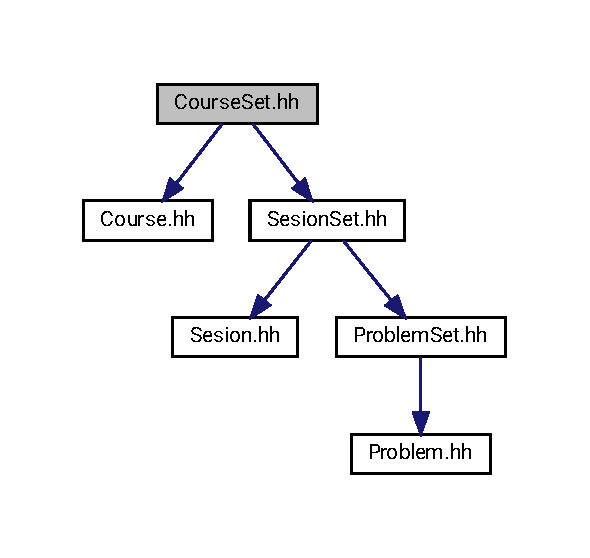
\includegraphics[width=283pt]{_course_set_8hh__incl}
\end{center}
\end{figure}
\subsection*{Clases}
\begin{DoxyCompactItemize}
\item 
class \mbox{\hyperlink{class_course_set}{Course\+Set}}
\begin{DoxyCompactList}\small\item\em Representa un conjunto de cursos. \end{DoxyCompactList}\end{DoxyCompactItemize}


\subsection{Descripción detallada}
Especificación de la clase Curso. 


\hypertarget{main_8cc}{}\section{Referencia del Archivo main.\+cc}
\label{main_8cc}\index{main.\+cc@{main.\+cc}}


Programa principal E\+V\+A\+L\+U\+A\+T\+OR\+: plataforma de gestión de problemas y cursos de programación.  


Dependencia gráfica adjunta para main.\+cc\+:\nopagebreak
\begin{figure}[H]
\begin{center}
\leavevmode
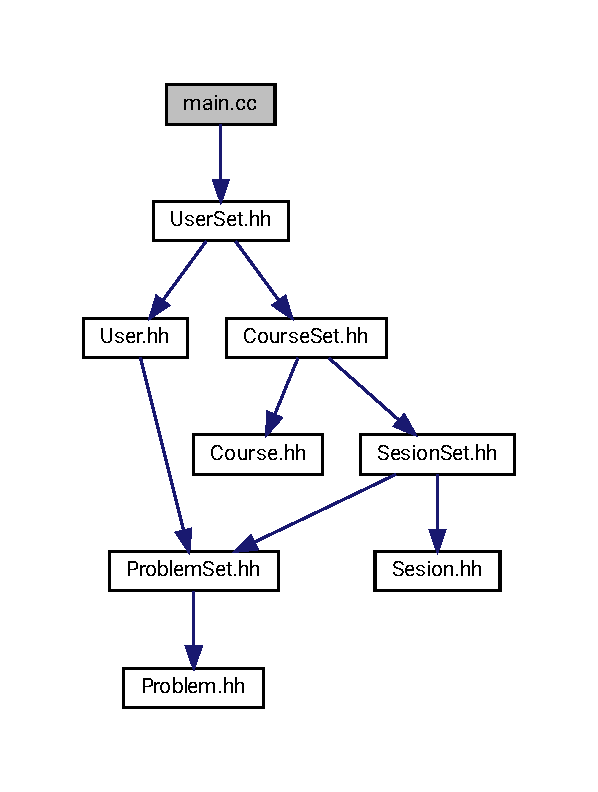
\includegraphics[width=287pt]{main_8cc__incl}
\end{center}
\end{figure}
\subsection*{defines}
\begin{DoxyCompactItemize}
\item 
\#define \mbox{\hyperlink{main_8cc_a77947d50d33173dbb8d2203ae806430f}{N\+U\+E\+V\+O\+\_\+\+P\+R\+O\+B\+L\+E\+MA}}~1
\item 
\#define \mbox{\hyperlink{main_8cc_a03b4a401073c8465967a2490e4255103}{N\+U\+E\+V\+A\+\_\+\+S\+E\+S\+I\+ON}}~2
\item 
\#define \mbox{\hyperlink{main_8cc_a23117f1ffed13aa567c085989e0b687b}{N\+U\+E\+V\+O\+\_\+\+C\+U\+R\+SO}}~3
\item 
\#define \mbox{\hyperlink{main_8cc_a111c69018aa752cf7d0b4485aaddd101}{A\+L\+T\+A\+\_\+\+U\+S\+U\+A\+R\+IO}}~4
\item 
\#define \mbox{\hyperlink{main_8cc_ada16e2b27577b1205b7cb1f67c1b7dfe}{B\+A\+J\+A\+\_\+\+U\+S\+U\+A\+R\+IO}}~5
\item 
\#define \mbox{\hyperlink{main_8cc_ac26ea1ba5fe2b5a7499861cacc35d771}{I\+N\+S\+C\+R\+I\+B\+I\+R\+\_\+\+C\+U\+R\+SO}}~6
\item 
\#define \mbox{\hyperlink{main_8cc_afa5e5ac0bff79d08b37a01b05c26c4a7}{C\+U\+R\+S\+O\+\_\+\+U\+S\+U\+A\+R\+IO}}~7
\item 
\#define \mbox{\hyperlink{main_8cc_ab607cfb91162b0667ab571d439b77e3d}{S\+E\+S\+I\+O\+N\+\_\+\+P\+R\+O\+B\+L\+E\+MA}}~8
\item 
\#define \mbox{\hyperlink{main_8cc_aa1bd243bac28c37c95e9e75af147a75b}{P\+R\+O\+B\+L\+E\+M\+A\+S\+\_\+\+R\+E\+S\+U\+E\+L\+T\+OS}}~9
\item 
\#define \mbox{\hyperlink{main_8cc_a55393525f368bcb01300b5a8ac6fc26d}{P\+R\+O\+B\+L\+E\+M\+A\+S\+\_\+\+E\+N\+V\+I\+A\+B\+L\+ES}}~10
\item 
\#define \mbox{\hyperlink{main_8cc_afed20d7a319638e05375f3ab0a52dc63}{E\+N\+V\+IO}}~11
\item 
\#define \mbox{\hyperlink{main_8cc_a386b604b5bbf5bef1a63fefca032c689}{L\+I\+S\+T\+A\+R\+\_\+\+P\+R\+O\+B\+L\+E\+M\+AS}}~12
\item 
\#define \mbox{\hyperlink{main_8cc_ac49f071eb90e5cc62da966a5c6e7ab66}{E\+S\+C\+R\+I\+B\+I\+R\+\_\+\+P\+R\+O\+B\+L\+E\+MA}}~13
\item 
\#define \mbox{\hyperlink{main_8cc_a51fa60d02e939c134b36fd61cb5c041b}{L\+I\+S\+T\+A\+R\+\_\+\+S\+E\+S\+I\+O\+N\+ES}}~14
\item 
\#define \mbox{\hyperlink{main_8cc_a111120c16f1bce9b9788628e86da4e81}{E\+S\+C\+R\+I\+B\+I\+R\+\_\+\+S\+E\+S\+I\+ON}}~15
\item 
\#define \mbox{\hyperlink{main_8cc_a6b65544bd990c1e167bacb4114190445}{L\+I\+S\+T\+A\+R\+\_\+\+C\+U\+R\+S\+OS}}~16
\item 
\#define \mbox{\hyperlink{main_8cc_ad225826f18bc59e4d712d11bdfeccf88}{E\+S\+C\+R\+I\+B\+I\+R\+\_\+\+C\+U\+R\+SO}}~17
\item 
\#define \mbox{\hyperlink{main_8cc_af56aa947fd7bd388c7cc8da566643a34}{L\+I\+S\+T\+A\+R\+\_\+\+U\+S\+U\+A\+R\+I\+OS}}~18
\item 
\#define \mbox{\hyperlink{main_8cc_aaf37e7516cb421e7d26279d92b2931f2}{E\+S\+C\+R\+I\+B\+I\+R\+\_\+\+U\+S\+U\+A\+R\+IO}}~19
\item 
\#define \mbox{\hyperlink{main_8cc_a1ce3da0d4a8e4638874faeae3b66fbcc}{F\+IN}}~20
\end{DoxyCompactItemize}
\subsection*{Funciones}
\begin{DoxyCompactItemize}
\item 
int \mbox{\hyperlink{main_8cc_ae66f6b31b5ad750f1fe042a706a4e3d4}{main}} ()
\end{DoxyCompactItemize}


\subsection{Descripción detallada}
Programa principal E\+V\+A\+L\+U\+A\+T\+OR\+: plataforma de gestión de problemas y cursos de programación. 



\subsection{Documentación de los \textquotesingle{}defines\textquotesingle{}}
\mbox{\Hypertarget{main_8cc_a77947d50d33173dbb8d2203ae806430f}\label{main_8cc_a77947d50d33173dbb8d2203ae806430f}} 
\index{main.\+cc@{main.\+cc}!N\+U\+E\+V\+O\+\_\+\+P\+R\+O\+B\+L\+E\+MA@{N\+U\+E\+V\+O\+\_\+\+P\+R\+O\+B\+L\+E\+MA}}
\index{N\+U\+E\+V\+O\+\_\+\+P\+R\+O\+B\+L\+E\+MA@{N\+U\+E\+V\+O\+\_\+\+P\+R\+O\+B\+L\+E\+MA}!main.\+cc@{main.\+cc}}
\subsubsection{\texorpdfstring{N\+U\+E\+V\+O\+\_\+\+P\+R\+O\+B\+L\+E\+MA}{NUEVO\_PROBLEMA}}
{\footnotesize\ttfamily \#define N\+U\+E\+V\+O\+\_\+\+P\+R\+O\+B\+L\+E\+MA~1}



Definición en la línea 22 del archivo main.\+cc.

\mbox{\Hypertarget{main_8cc_a03b4a401073c8465967a2490e4255103}\label{main_8cc_a03b4a401073c8465967a2490e4255103}} 
\index{main.\+cc@{main.\+cc}!N\+U\+E\+V\+A\+\_\+\+S\+E\+S\+I\+ON@{N\+U\+E\+V\+A\+\_\+\+S\+E\+S\+I\+ON}}
\index{N\+U\+E\+V\+A\+\_\+\+S\+E\+S\+I\+ON@{N\+U\+E\+V\+A\+\_\+\+S\+E\+S\+I\+ON}!main.\+cc@{main.\+cc}}
\subsubsection{\texorpdfstring{N\+U\+E\+V\+A\+\_\+\+S\+E\+S\+I\+ON}{NUEVA\_SESION}}
{\footnotesize\ttfamily \#define N\+U\+E\+V\+A\+\_\+\+S\+E\+S\+I\+ON~2}



Definición en la línea 23 del archivo main.\+cc.

\mbox{\Hypertarget{main_8cc_a23117f1ffed13aa567c085989e0b687b}\label{main_8cc_a23117f1ffed13aa567c085989e0b687b}} 
\index{main.\+cc@{main.\+cc}!N\+U\+E\+V\+O\+\_\+\+C\+U\+R\+SO@{N\+U\+E\+V\+O\+\_\+\+C\+U\+R\+SO}}
\index{N\+U\+E\+V\+O\+\_\+\+C\+U\+R\+SO@{N\+U\+E\+V\+O\+\_\+\+C\+U\+R\+SO}!main.\+cc@{main.\+cc}}
\subsubsection{\texorpdfstring{N\+U\+E\+V\+O\+\_\+\+C\+U\+R\+SO}{NUEVO\_CURSO}}
{\footnotesize\ttfamily \#define N\+U\+E\+V\+O\+\_\+\+C\+U\+R\+SO~3}



Definición en la línea 24 del archivo main.\+cc.

\mbox{\Hypertarget{main_8cc_a111c69018aa752cf7d0b4485aaddd101}\label{main_8cc_a111c69018aa752cf7d0b4485aaddd101}} 
\index{main.\+cc@{main.\+cc}!A\+L\+T\+A\+\_\+\+U\+S\+U\+A\+R\+IO@{A\+L\+T\+A\+\_\+\+U\+S\+U\+A\+R\+IO}}
\index{A\+L\+T\+A\+\_\+\+U\+S\+U\+A\+R\+IO@{A\+L\+T\+A\+\_\+\+U\+S\+U\+A\+R\+IO}!main.\+cc@{main.\+cc}}
\subsubsection{\texorpdfstring{A\+L\+T\+A\+\_\+\+U\+S\+U\+A\+R\+IO}{ALTA\_USUARIO}}
{\footnotesize\ttfamily \#define A\+L\+T\+A\+\_\+\+U\+S\+U\+A\+R\+IO~4}



Definición en la línea 25 del archivo main.\+cc.

\mbox{\Hypertarget{main_8cc_ada16e2b27577b1205b7cb1f67c1b7dfe}\label{main_8cc_ada16e2b27577b1205b7cb1f67c1b7dfe}} 
\index{main.\+cc@{main.\+cc}!B\+A\+J\+A\+\_\+\+U\+S\+U\+A\+R\+IO@{B\+A\+J\+A\+\_\+\+U\+S\+U\+A\+R\+IO}}
\index{B\+A\+J\+A\+\_\+\+U\+S\+U\+A\+R\+IO@{B\+A\+J\+A\+\_\+\+U\+S\+U\+A\+R\+IO}!main.\+cc@{main.\+cc}}
\subsubsection{\texorpdfstring{B\+A\+J\+A\+\_\+\+U\+S\+U\+A\+R\+IO}{BAJA\_USUARIO}}
{\footnotesize\ttfamily \#define B\+A\+J\+A\+\_\+\+U\+S\+U\+A\+R\+IO~5}



Definición en la línea 26 del archivo main.\+cc.

\mbox{\Hypertarget{main_8cc_ac26ea1ba5fe2b5a7499861cacc35d771}\label{main_8cc_ac26ea1ba5fe2b5a7499861cacc35d771}} 
\index{main.\+cc@{main.\+cc}!I\+N\+S\+C\+R\+I\+B\+I\+R\+\_\+\+C\+U\+R\+SO@{I\+N\+S\+C\+R\+I\+B\+I\+R\+\_\+\+C\+U\+R\+SO}}
\index{I\+N\+S\+C\+R\+I\+B\+I\+R\+\_\+\+C\+U\+R\+SO@{I\+N\+S\+C\+R\+I\+B\+I\+R\+\_\+\+C\+U\+R\+SO}!main.\+cc@{main.\+cc}}
\subsubsection{\texorpdfstring{I\+N\+S\+C\+R\+I\+B\+I\+R\+\_\+\+C\+U\+R\+SO}{INSCRIBIR\_CURSO}}
{\footnotesize\ttfamily \#define I\+N\+S\+C\+R\+I\+B\+I\+R\+\_\+\+C\+U\+R\+SO~6}



Definición en la línea 27 del archivo main.\+cc.

\mbox{\Hypertarget{main_8cc_afa5e5ac0bff79d08b37a01b05c26c4a7}\label{main_8cc_afa5e5ac0bff79d08b37a01b05c26c4a7}} 
\index{main.\+cc@{main.\+cc}!C\+U\+R\+S\+O\+\_\+\+U\+S\+U\+A\+R\+IO@{C\+U\+R\+S\+O\+\_\+\+U\+S\+U\+A\+R\+IO}}
\index{C\+U\+R\+S\+O\+\_\+\+U\+S\+U\+A\+R\+IO@{C\+U\+R\+S\+O\+\_\+\+U\+S\+U\+A\+R\+IO}!main.\+cc@{main.\+cc}}
\subsubsection{\texorpdfstring{C\+U\+R\+S\+O\+\_\+\+U\+S\+U\+A\+R\+IO}{CURSO\_USUARIO}}
{\footnotesize\ttfamily \#define C\+U\+R\+S\+O\+\_\+\+U\+S\+U\+A\+R\+IO~7}



Definición en la línea 28 del archivo main.\+cc.

\mbox{\Hypertarget{main_8cc_ab607cfb91162b0667ab571d439b77e3d}\label{main_8cc_ab607cfb91162b0667ab571d439b77e3d}} 
\index{main.\+cc@{main.\+cc}!S\+E\+S\+I\+O\+N\+\_\+\+P\+R\+O\+B\+L\+E\+MA@{S\+E\+S\+I\+O\+N\+\_\+\+P\+R\+O\+B\+L\+E\+MA}}
\index{S\+E\+S\+I\+O\+N\+\_\+\+P\+R\+O\+B\+L\+E\+MA@{S\+E\+S\+I\+O\+N\+\_\+\+P\+R\+O\+B\+L\+E\+MA}!main.\+cc@{main.\+cc}}
\subsubsection{\texorpdfstring{S\+E\+S\+I\+O\+N\+\_\+\+P\+R\+O\+B\+L\+E\+MA}{SESION\_PROBLEMA}}
{\footnotesize\ttfamily \#define S\+E\+S\+I\+O\+N\+\_\+\+P\+R\+O\+B\+L\+E\+MA~8}



Definición en la línea 29 del archivo main.\+cc.

\mbox{\Hypertarget{main_8cc_aa1bd243bac28c37c95e9e75af147a75b}\label{main_8cc_aa1bd243bac28c37c95e9e75af147a75b}} 
\index{main.\+cc@{main.\+cc}!P\+R\+O\+B\+L\+E\+M\+A\+S\+\_\+\+R\+E\+S\+U\+E\+L\+T\+OS@{P\+R\+O\+B\+L\+E\+M\+A\+S\+\_\+\+R\+E\+S\+U\+E\+L\+T\+OS}}
\index{P\+R\+O\+B\+L\+E\+M\+A\+S\+\_\+\+R\+E\+S\+U\+E\+L\+T\+OS@{P\+R\+O\+B\+L\+E\+M\+A\+S\+\_\+\+R\+E\+S\+U\+E\+L\+T\+OS}!main.\+cc@{main.\+cc}}
\subsubsection{\texorpdfstring{P\+R\+O\+B\+L\+E\+M\+A\+S\+\_\+\+R\+E\+S\+U\+E\+L\+T\+OS}{PROBLEMAS\_RESUELTOS}}
{\footnotesize\ttfamily \#define P\+R\+O\+B\+L\+E\+M\+A\+S\+\_\+\+R\+E\+S\+U\+E\+L\+T\+OS~9}



Definición en la línea 30 del archivo main.\+cc.

\mbox{\Hypertarget{main_8cc_a55393525f368bcb01300b5a8ac6fc26d}\label{main_8cc_a55393525f368bcb01300b5a8ac6fc26d}} 
\index{main.\+cc@{main.\+cc}!P\+R\+O\+B\+L\+E\+M\+A\+S\+\_\+\+E\+N\+V\+I\+A\+B\+L\+ES@{P\+R\+O\+B\+L\+E\+M\+A\+S\+\_\+\+E\+N\+V\+I\+A\+B\+L\+ES}}
\index{P\+R\+O\+B\+L\+E\+M\+A\+S\+\_\+\+E\+N\+V\+I\+A\+B\+L\+ES@{P\+R\+O\+B\+L\+E\+M\+A\+S\+\_\+\+E\+N\+V\+I\+A\+B\+L\+ES}!main.\+cc@{main.\+cc}}
\subsubsection{\texorpdfstring{P\+R\+O\+B\+L\+E\+M\+A\+S\+\_\+\+E\+N\+V\+I\+A\+B\+L\+ES}{PROBLEMAS\_ENVIABLES}}
{\footnotesize\ttfamily \#define P\+R\+O\+B\+L\+E\+M\+A\+S\+\_\+\+E\+N\+V\+I\+A\+B\+L\+ES~10}



Definición en la línea 31 del archivo main.\+cc.

\mbox{\Hypertarget{main_8cc_afed20d7a319638e05375f3ab0a52dc63}\label{main_8cc_afed20d7a319638e05375f3ab0a52dc63}} 
\index{main.\+cc@{main.\+cc}!E\+N\+V\+IO@{E\+N\+V\+IO}}
\index{E\+N\+V\+IO@{E\+N\+V\+IO}!main.\+cc@{main.\+cc}}
\subsubsection{\texorpdfstring{E\+N\+V\+IO}{ENVIO}}
{\footnotesize\ttfamily \#define E\+N\+V\+IO~11}



Definición en la línea 32 del archivo main.\+cc.

\mbox{\Hypertarget{main_8cc_a386b604b5bbf5bef1a63fefca032c689}\label{main_8cc_a386b604b5bbf5bef1a63fefca032c689}} 
\index{main.\+cc@{main.\+cc}!L\+I\+S\+T\+A\+R\+\_\+\+P\+R\+O\+B\+L\+E\+M\+AS@{L\+I\+S\+T\+A\+R\+\_\+\+P\+R\+O\+B\+L\+E\+M\+AS}}
\index{L\+I\+S\+T\+A\+R\+\_\+\+P\+R\+O\+B\+L\+E\+M\+AS@{L\+I\+S\+T\+A\+R\+\_\+\+P\+R\+O\+B\+L\+E\+M\+AS}!main.\+cc@{main.\+cc}}
\subsubsection{\texorpdfstring{L\+I\+S\+T\+A\+R\+\_\+\+P\+R\+O\+B\+L\+E\+M\+AS}{LISTAR\_PROBLEMAS}}
{\footnotesize\ttfamily \#define L\+I\+S\+T\+A\+R\+\_\+\+P\+R\+O\+B\+L\+E\+M\+AS~12}



Definición en la línea 33 del archivo main.\+cc.

\mbox{\Hypertarget{main_8cc_ac49f071eb90e5cc62da966a5c6e7ab66}\label{main_8cc_ac49f071eb90e5cc62da966a5c6e7ab66}} 
\index{main.\+cc@{main.\+cc}!E\+S\+C\+R\+I\+B\+I\+R\+\_\+\+P\+R\+O\+B\+L\+E\+MA@{E\+S\+C\+R\+I\+B\+I\+R\+\_\+\+P\+R\+O\+B\+L\+E\+MA}}
\index{E\+S\+C\+R\+I\+B\+I\+R\+\_\+\+P\+R\+O\+B\+L\+E\+MA@{E\+S\+C\+R\+I\+B\+I\+R\+\_\+\+P\+R\+O\+B\+L\+E\+MA}!main.\+cc@{main.\+cc}}
\subsubsection{\texorpdfstring{E\+S\+C\+R\+I\+B\+I\+R\+\_\+\+P\+R\+O\+B\+L\+E\+MA}{ESCRIBIR\_PROBLEMA}}
{\footnotesize\ttfamily \#define E\+S\+C\+R\+I\+B\+I\+R\+\_\+\+P\+R\+O\+B\+L\+E\+MA~13}



Definición en la línea 34 del archivo main.\+cc.

\mbox{\Hypertarget{main_8cc_a51fa60d02e939c134b36fd61cb5c041b}\label{main_8cc_a51fa60d02e939c134b36fd61cb5c041b}} 
\index{main.\+cc@{main.\+cc}!L\+I\+S\+T\+A\+R\+\_\+\+S\+E\+S\+I\+O\+N\+ES@{L\+I\+S\+T\+A\+R\+\_\+\+S\+E\+S\+I\+O\+N\+ES}}
\index{L\+I\+S\+T\+A\+R\+\_\+\+S\+E\+S\+I\+O\+N\+ES@{L\+I\+S\+T\+A\+R\+\_\+\+S\+E\+S\+I\+O\+N\+ES}!main.\+cc@{main.\+cc}}
\subsubsection{\texorpdfstring{L\+I\+S\+T\+A\+R\+\_\+\+S\+E\+S\+I\+O\+N\+ES}{LISTAR\_SESIONES}}
{\footnotesize\ttfamily \#define L\+I\+S\+T\+A\+R\+\_\+\+S\+E\+S\+I\+O\+N\+ES~14}



Definición en la línea 35 del archivo main.\+cc.

\mbox{\Hypertarget{main_8cc_a111120c16f1bce9b9788628e86da4e81}\label{main_8cc_a111120c16f1bce9b9788628e86da4e81}} 
\index{main.\+cc@{main.\+cc}!E\+S\+C\+R\+I\+B\+I\+R\+\_\+\+S\+E\+S\+I\+ON@{E\+S\+C\+R\+I\+B\+I\+R\+\_\+\+S\+E\+S\+I\+ON}}
\index{E\+S\+C\+R\+I\+B\+I\+R\+\_\+\+S\+E\+S\+I\+ON@{E\+S\+C\+R\+I\+B\+I\+R\+\_\+\+S\+E\+S\+I\+ON}!main.\+cc@{main.\+cc}}
\subsubsection{\texorpdfstring{E\+S\+C\+R\+I\+B\+I\+R\+\_\+\+S\+E\+S\+I\+ON}{ESCRIBIR\_SESION}}
{\footnotesize\ttfamily \#define E\+S\+C\+R\+I\+B\+I\+R\+\_\+\+S\+E\+S\+I\+ON~15}



Definición en la línea 36 del archivo main.\+cc.

\mbox{\Hypertarget{main_8cc_a6b65544bd990c1e167bacb4114190445}\label{main_8cc_a6b65544bd990c1e167bacb4114190445}} 
\index{main.\+cc@{main.\+cc}!L\+I\+S\+T\+A\+R\+\_\+\+C\+U\+R\+S\+OS@{L\+I\+S\+T\+A\+R\+\_\+\+C\+U\+R\+S\+OS}}
\index{L\+I\+S\+T\+A\+R\+\_\+\+C\+U\+R\+S\+OS@{L\+I\+S\+T\+A\+R\+\_\+\+C\+U\+R\+S\+OS}!main.\+cc@{main.\+cc}}
\subsubsection{\texorpdfstring{L\+I\+S\+T\+A\+R\+\_\+\+C\+U\+R\+S\+OS}{LISTAR\_CURSOS}}
{\footnotesize\ttfamily \#define L\+I\+S\+T\+A\+R\+\_\+\+C\+U\+R\+S\+OS~16}



Definición en la línea 37 del archivo main.\+cc.

\mbox{\Hypertarget{main_8cc_ad225826f18bc59e4d712d11bdfeccf88}\label{main_8cc_ad225826f18bc59e4d712d11bdfeccf88}} 
\index{main.\+cc@{main.\+cc}!E\+S\+C\+R\+I\+B\+I\+R\+\_\+\+C\+U\+R\+SO@{E\+S\+C\+R\+I\+B\+I\+R\+\_\+\+C\+U\+R\+SO}}
\index{E\+S\+C\+R\+I\+B\+I\+R\+\_\+\+C\+U\+R\+SO@{E\+S\+C\+R\+I\+B\+I\+R\+\_\+\+C\+U\+R\+SO}!main.\+cc@{main.\+cc}}
\subsubsection{\texorpdfstring{E\+S\+C\+R\+I\+B\+I\+R\+\_\+\+C\+U\+R\+SO}{ESCRIBIR\_CURSO}}
{\footnotesize\ttfamily \#define E\+S\+C\+R\+I\+B\+I\+R\+\_\+\+C\+U\+R\+SO~17}



Definición en la línea 38 del archivo main.\+cc.

\mbox{\Hypertarget{main_8cc_af56aa947fd7bd388c7cc8da566643a34}\label{main_8cc_af56aa947fd7bd388c7cc8da566643a34}} 
\index{main.\+cc@{main.\+cc}!L\+I\+S\+T\+A\+R\+\_\+\+U\+S\+U\+A\+R\+I\+OS@{L\+I\+S\+T\+A\+R\+\_\+\+U\+S\+U\+A\+R\+I\+OS}}
\index{L\+I\+S\+T\+A\+R\+\_\+\+U\+S\+U\+A\+R\+I\+OS@{L\+I\+S\+T\+A\+R\+\_\+\+U\+S\+U\+A\+R\+I\+OS}!main.\+cc@{main.\+cc}}
\subsubsection{\texorpdfstring{L\+I\+S\+T\+A\+R\+\_\+\+U\+S\+U\+A\+R\+I\+OS}{LISTAR\_USUARIOS}}
{\footnotesize\ttfamily \#define L\+I\+S\+T\+A\+R\+\_\+\+U\+S\+U\+A\+R\+I\+OS~18}



Definición en la línea 39 del archivo main.\+cc.

\mbox{\Hypertarget{main_8cc_aaf37e7516cb421e7d26279d92b2931f2}\label{main_8cc_aaf37e7516cb421e7d26279d92b2931f2}} 
\index{main.\+cc@{main.\+cc}!E\+S\+C\+R\+I\+B\+I\+R\+\_\+\+U\+S\+U\+A\+R\+IO@{E\+S\+C\+R\+I\+B\+I\+R\+\_\+\+U\+S\+U\+A\+R\+IO}}
\index{E\+S\+C\+R\+I\+B\+I\+R\+\_\+\+U\+S\+U\+A\+R\+IO@{E\+S\+C\+R\+I\+B\+I\+R\+\_\+\+U\+S\+U\+A\+R\+IO}!main.\+cc@{main.\+cc}}
\subsubsection{\texorpdfstring{E\+S\+C\+R\+I\+B\+I\+R\+\_\+\+U\+S\+U\+A\+R\+IO}{ESCRIBIR\_USUARIO}}
{\footnotesize\ttfamily \#define E\+S\+C\+R\+I\+B\+I\+R\+\_\+\+U\+S\+U\+A\+R\+IO~19}



Definición en la línea 40 del archivo main.\+cc.

\mbox{\Hypertarget{main_8cc_a1ce3da0d4a8e4638874faeae3b66fbcc}\label{main_8cc_a1ce3da0d4a8e4638874faeae3b66fbcc}} 
\index{main.\+cc@{main.\+cc}!F\+IN@{F\+IN}}
\index{F\+IN@{F\+IN}!main.\+cc@{main.\+cc}}
\subsubsection{\texorpdfstring{F\+IN}{FIN}}
{\footnotesize\ttfamily \#define F\+IN~20}



Definición en la línea 41 del archivo main.\+cc.



\subsection{Documentación de las funciones}
\mbox{\Hypertarget{main_8cc_ae66f6b31b5ad750f1fe042a706a4e3d4}\label{main_8cc_ae66f6b31b5ad750f1fe042a706a4e3d4}} 
\index{main.\+cc@{main.\+cc}!main@{main}}
\index{main@{main}!main.\+cc@{main.\+cc}}
\subsubsection{\texorpdfstring{main()}{main()}}
{\footnotesize\ttfamily int main (\begin{DoxyParamCaption}{ }\end{DoxyParamCaption})}



Definición en la línea 43 del archivo main.\+cc.


\begin{DoxyCode}
43            \{
44     
45     \textcolor{comment}{//INICIALIZAR MAP DE COMANDOS}
46     map<string, int> comandos;
47     comandos[\textcolor{stringliteral}{"nuevo\_problema"}]      = \mbox{\hyperlink{main_8cc_a77947d50d33173dbb8d2203ae806430f}{NUEVO\_PROBLEMA}};
48     comandos[\textcolor{stringliteral}{"np"}]                  = \mbox{\hyperlink{main_8cc_a77947d50d33173dbb8d2203ae806430f}{NUEVO\_PROBLEMA}};
49     comandos[\textcolor{stringliteral}{"nueva\_sesion"}]        = \mbox{\hyperlink{main_8cc_a03b4a401073c8465967a2490e4255103}{NUEVA\_SESION}};
50     comandos[\textcolor{stringliteral}{"ns"}]                  = \mbox{\hyperlink{main_8cc_a03b4a401073c8465967a2490e4255103}{NUEVA\_SESION}};
51     comandos[\textcolor{stringliteral}{"nuevo\_curso"}]         = \mbox{\hyperlink{main_8cc_a23117f1ffed13aa567c085989e0b687b}{NUEVO\_CURSO}};
52     comandos[\textcolor{stringliteral}{"nc"}]                  = \mbox{\hyperlink{main_8cc_a23117f1ffed13aa567c085989e0b687b}{NUEVO\_CURSO}};
53     comandos[\textcolor{stringliteral}{"alta\_usuario"}]        = \mbox{\hyperlink{main_8cc_a111c69018aa752cf7d0b4485aaddd101}{ALTA\_USUARIO}};
54     comandos[\textcolor{stringliteral}{"a"}]                   = \mbox{\hyperlink{main_8cc_a111c69018aa752cf7d0b4485aaddd101}{ALTA\_USUARIO}};
55     comandos[\textcolor{stringliteral}{"baja\_usuario"}]        = \mbox{\hyperlink{main_8cc_ada16e2b27577b1205b7cb1f67c1b7dfe}{BAJA\_USUARIO}};
56     comandos[\textcolor{stringliteral}{"b"}]                   = \mbox{\hyperlink{main_8cc_ada16e2b27577b1205b7cb1f67c1b7dfe}{BAJA\_USUARIO}};
57     comandos[\textcolor{stringliteral}{"inscribir\_curso"}]     = \mbox{\hyperlink{main_8cc_ac26ea1ba5fe2b5a7499861cacc35d771}{INSCRIBIR\_CURSO}};
58     comandos[\textcolor{stringliteral}{"i"}]                   = \mbox{\hyperlink{main_8cc_ac26ea1ba5fe2b5a7499861cacc35d771}{INSCRIBIR\_CURSO}};
59     comandos[\textcolor{stringliteral}{"curso\_usuario"}]       = \mbox{\hyperlink{main_8cc_afa5e5ac0bff79d08b37a01b05c26c4a7}{CURSO\_USUARIO}};
60     comandos[\textcolor{stringliteral}{"cu"}]                  = \mbox{\hyperlink{main_8cc_afa5e5ac0bff79d08b37a01b05c26c4a7}{CURSO\_USUARIO}};
61     comandos[\textcolor{stringliteral}{"sesion\_problema"}]     = \mbox{\hyperlink{main_8cc_ab607cfb91162b0667ab571d439b77e3d}{SESION\_PROBLEMA}};
62     comandos[\textcolor{stringliteral}{"sp"}]                  = \mbox{\hyperlink{main_8cc_ab607cfb91162b0667ab571d439b77e3d}{SESION\_PROBLEMA}};
63     comandos[\textcolor{stringliteral}{"problemas\_resueltos"}] = \mbox{\hyperlink{main_8cc_aa1bd243bac28c37c95e9e75af147a75b}{PROBLEMAS\_RESUELTOS}};
64     comandos[\textcolor{stringliteral}{"pr"}]                  = \mbox{\hyperlink{main_8cc_aa1bd243bac28c37c95e9e75af147a75b}{PROBLEMAS\_RESUELTOS}};
65     comandos[\textcolor{stringliteral}{"problemas\_enviables"}] = \mbox{\hyperlink{main_8cc_a55393525f368bcb01300b5a8ac6fc26d}{PROBLEMAS\_ENVIABLES}};
66     comandos[\textcolor{stringliteral}{"pe"}]                  = \mbox{\hyperlink{main_8cc_a55393525f368bcb01300b5a8ac6fc26d}{PROBLEMAS\_ENVIABLES}};
67     comandos[\textcolor{stringliteral}{"envio"}]               = \mbox{\hyperlink{main_8cc_afed20d7a319638e05375f3ab0a52dc63}{ENVIO}};
68     comandos[\textcolor{stringliteral}{"e"}]                   = \mbox{\hyperlink{main_8cc_afed20d7a319638e05375f3ab0a52dc63}{ENVIO}};
69     comandos[\textcolor{stringliteral}{"listar\_problemas"}]    = \mbox{\hyperlink{main_8cc_a386b604b5bbf5bef1a63fefca032c689}{LISTAR\_PROBLEMAS}};
70     comandos[\textcolor{stringliteral}{"lp"}]                  = \mbox{\hyperlink{main_8cc_a386b604b5bbf5bef1a63fefca032c689}{LISTAR\_PROBLEMAS}};
71     comandos[\textcolor{stringliteral}{"escribir\_problema"}]   = \mbox{\hyperlink{main_8cc_ac49f071eb90e5cc62da966a5c6e7ab66}{ESCRIBIR\_PROBLEMA}};
72     comandos[\textcolor{stringliteral}{"ep"}]                  = \mbox{\hyperlink{main_8cc_ac49f071eb90e5cc62da966a5c6e7ab66}{ESCRIBIR\_PROBLEMA}};
73     comandos[\textcolor{stringliteral}{"listar\_sesiones"}]     = \mbox{\hyperlink{main_8cc_a51fa60d02e939c134b36fd61cb5c041b}{LISTAR\_SESIONES}};
74     comandos[\textcolor{stringliteral}{"ls"}]                  = \mbox{\hyperlink{main_8cc_a51fa60d02e939c134b36fd61cb5c041b}{LISTAR\_SESIONES}};
75     comandos[\textcolor{stringliteral}{"escribir\_sesion"}]     = \mbox{\hyperlink{main_8cc_a111120c16f1bce9b9788628e86da4e81}{ESCRIBIR\_SESION}};
76     comandos[\textcolor{stringliteral}{"es"}]                  = \mbox{\hyperlink{main_8cc_a111120c16f1bce9b9788628e86da4e81}{ESCRIBIR\_SESION}};
77     comandos[\textcolor{stringliteral}{"listar\_cursos"}]       = \mbox{\hyperlink{main_8cc_a6b65544bd990c1e167bacb4114190445}{LISTAR\_CURSOS}};
78     comandos[\textcolor{stringliteral}{"lc"}]                  = \mbox{\hyperlink{main_8cc_a6b65544bd990c1e167bacb4114190445}{LISTAR\_CURSOS}};
79     comandos[\textcolor{stringliteral}{"escribir\_curso"}]      = \mbox{\hyperlink{main_8cc_ad225826f18bc59e4d712d11bdfeccf88}{ESCRIBIR\_CURSO}};
80     comandos[\textcolor{stringliteral}{"ec"}]                  = \mbox{\hyperlink{main_8cc_ad225826f18bc59e4d712d11bdfeccf88}{ESCRIBIR\_CURSO}};
81     comandos[\textcolor{stringliteral}{"listar\_usuarios"}]     = \mbox{\hyperlink{main_8cc_af56aa947fd7bd388c7cc8da566643a34}{LISTAR\_USUARIOS}};
82     comandos[\textcolor{stringliteral}{"lu"}]                  = \mbox{\hyperlink{main_8cc_af56aa947fd7bd388c7cc8da566643a34}{LISTAR\_USUARIOS}};
83     comandos[\textcolor{stringliteral}{"escribir\_usuario"}]    = \mbox{\hyperlink{main_8cc_aaf37e7516cb421e7d26279d92b2931f2}{ESCRIBIR\_USUARIO}};
84     comandos[\textcolor{stringliteral}{"eu"}]                  = \mbox{\hyperlink{main_8cc_aaf37e7516cb421e7d26279d92b2931f2}{ESCRIBIR\_USUARIO}};
85     comandos[\textcolor{stringliteral}{"fin"}]                 = \mbox{\hyperlink{main_8cc_a1ce3da0d4a8e4638874faeae3b66fbcc}{FIN}} ;
86 
87     \textcolor{comment}{//INICIALIZAR OBJETOS}
88     \mbox{\hyperlink{class_problem_set}{ProblemSet}}  problemas;
89     \mbox{\hyperlink{class_sesion_set}{SesionSet}}   sesiones;
90     \mbox{\hyperlink{class_course_set}{CourseSet}}   cursos;
91     \mbox{\hyperlink{class_user_set}{UserSet}}     usuarios;
92     
93     problemas.\mbox{\hyperlink{class_problem_set_adac211be4426d3b9395de055bbf43131}{AddFromConsole}}();
94     sesiones.\mbox{\hyperlink{class_sesion_set_a683506f0dc85b15392e77ebe4e6cc266}{AddFromConsole}}();    
95     cursos.\mbox{\hyperlink{class_course_set_aee9d2b96c43a828049e02205736a4982}{AddFromConsole}}();
96     usuarios.\mbox{\hyperlink{class_user_set_a4618efff11bc85371b754ee58e138ba4}{AddFromConsole}}();
97     
98     \textcolor{comment}{//VARIABLES AUXILIARES}
99     \textcolor{keywordtype}{string} comando;
100     \textcolor{keywordtype}{bool} pedir\_comando = \textcolor{keyword}{true};
101     \textcolor{keywordtype}{string} p, s, u;
102     \textcolor{keywordtype}{int} c;
103     
104     \textcolor{comment}{//SWITCH CASE (main body)}
105     \textcolor{keywordflow}{while} (pedir\_comando) \{
106         cin >> comando;
107         \textcolor{keywordflow}{if} (comandos.find(comando) != comandos.end()) \{
108             \textcolor{comment}{// Comando válido}
109             \textcolor{keywordflow}{switch} (comandos[comando]) \{
110                 
111                 \textcolor{keywordflow}{case} \mbox{\hyperlink{main_8cc_a77947d50d33173dbb8d2203ae806430f}{NUEVO\_PROBLEMA}}:
112                     cin >> p;
113                     \textcolor{keywordflow}{if} (problemas.\mbox{\hyperlink{class_problem_set_ae41f8319bc9355824cf982879c7d0453}{Add}}(p) == -1)
114                         cout << \textcolor{stringliteral}{"Error al introducir el problema "} << p << \textcolor{stringliteral}{", este ya existe."} << endl;
115                     \textcolor{keywordflow}{else} 
116                         cout << \textcolor{stringliteral}{"Número de problemas: "} << problemas.\mbox{\hyperlink{class_problem_set_ac173526274dc6d5f88623c3dd2630cd6}{Size}}() << \textcolor{stringliteral}{"."} <<  endl;           
              
117                     \textcolor{keywordflow}{break};
118                 
119                     
120                 \textcolor{keywordflow}{case} \mbox{\hyperlink{main_8cc_a03b4a401073c8465967a2490e4255103}{NUEVA\_SESION}}:
121                     cin >> s;
122                     \textcolor{keywordflow}{if} (sesiones.\mbox{\hyperlink{class_sesion_set_a74a8b110d55902c12d867e090c6092c2}{AddOneFromConsole}}(s) == -1) 
123                         \textcolor{comment}{// AddOneFromConsole comprueba si s existe. }
124                         \textcolor{comment}{// - Si existe, pedirá a través de la consola los identificadores de problemas,
       pero no creará el BinTree ya que la sesion no se creará al estar repetida. Retornará -1}
125                         \textcolor{comment}{// - Si no existe la sesión, pedirá a través de la consola los identificadores de
       problemas para construir el BinTree dentro de la sesion creada. Retornará 0 (OK)}
126                         
127                         cout << \textcolor{stringliteral}{"Error al introducir la sesion "} << s << \textcolor{stringliteral}{", esta ya existe."} << endl;
128                     \textcolor{keywordflow}{else}   
129                         cout << \textcolor{stringliteral}{"Número de sesiones: "} << sesiones.\mbox{\hyperlink{class_sesion_set_aa4cf0fbea2b9f9b6322390fc8b4a1b4c}{Size}}() << \textcolor{stringliteral}{"."} << endl;
130                     \textcolor{keywordflow}{break};
131                     
132                     
133                 \textcolor{keywordflow}{case} \mbox{\hyperlink{main_8cc_a23117f1ffed13aa567c085989e0b687b}{NUEVO\_CURSO}}:
134                     \textcolor{keywordflow}{if} (cursos.\mbox{\hyperlink{class_course_set_ae74448a3ba72c104d4f35abf41d47b0e}{AddOneFromConsole}}() == -1)
135                         \textcolor{comment}{// AddOneFromConsole pedirá el número de sesiones del curso, y posteriormente
       pedirá los strings de todas las sesiones. }
136                         \textcolor{comment}{// - Si en el nuevo curso hay intersección de problemas entre sesiones, no se
       creará el curso. Retornará -1}
137                         \textcolor{comment}{// - Si no hay intersección de problemas entre sesiones, se creará el curso. Dentro
       del curso rellenaremos el curso\_sesion\_map, con key id\_problema(string), y value id\_sesion(string). }
138                         \textcolor{comment}{//      Después de añadirlo, el identificador del curso será cursos.Size().
       Retornará 0 (Ok)}
139                         cout << \textcolor{stringliteral}{"Error al introducir el curso."} << endl;
140                     \textcolor{keywordflow}{else}   
141                         cout << \textcolor{stringliteral}{"Nuevo curso creado con identificador: "} << cursos.
      \mbox{\hyperlink{class_course_set_ac255028f38ba0b5b3ef1994e2a9a6c6f}{Size}}() << \textcolor{stringliteral}{"."} << endl;
142                     \textcolor{keywordflow}{break};                  
143                     
144                     
145                 \textcolor{keywordflow}{case} \mbox{\hyperlink{main_8cc_a111c69018aa752cf7d0b4485aaddd101}{ALTA\_USUARIO}}:
146                     cin >> u;
147                     \textcolor{keywordflow}{if} (usuarios.\mbox{\hyperlink{class_user_set_af0b143d52582d95f08ad92c9eee64394}{Add}}(u) == -1)
148                         cout << \textcolor{stringliteral}{"Error, no se puede dar de alta a un usuario ya existente."} << endl;
149                     \textcolor{keywordflow}{else} 
150                         
151                         cout << \textcolor{stringliteral}{"Número de usuarios: "} << usuarios.\mbox{\hyperlink{class_user_set_a2474615357041661d6c00ce66209e747}{Size}}() << \textcolor{stringliteral}{"."} << endl; 
152                     \textcolor{keywordflow}{break};
153                     
154                     
155                 \textcolor{keywordflow}{case} \mbox{\hyperlink{main_8cc_ada16e2b27577b1205b7cb1f67c1b7dfe}{BAJA\_USUARIO}}:
156                     cin >> u;
157                     \textcolor{keywordflow}{if} (not usuarios.\mbox{\hyperlink{class_user_set_a71ead20f591befdba9f6a1e524fa3271}{Exist}}(u))
158                          cout << \textcolor{stringliteral}{"Error, no se puede dar de baja a un usuario inexistente."} << endl;
159                     \textcolor{keywordflow}{else} \{
160                         usuarios.\mbox{\hyperlink{class_user_set_a9a548c48abafd33e8460d9e8a9e40170}{Delete}}(u);                                                          
                  
161                         \textcolor{comment}{//borrar todo lo referente al usuario. Si luego se da de alta un usuario con el
       mismo id es como si el anterior no hubiese existido.}
162                         \textcolor{comment}{// Tener en cuenta que si el usuario está inscrito en un curso (variable
       curso\_incrito != 0), se ha de decrementar el número de usuarios inscritos del curso }
163                         \textcolor{comment}{// con id=curso\_inscrito (cursos.DecNumUsersIn(curso\_inscrito)) }
164                         cout << \textcolor{stringliteral}{"Número de usuarios: "} << usuarios.\mbox{\hyperlink{class_user_set_a2474615357041661d6c00ce66209e747}{Size}}() << \textcolor{stringliteral}{"."} << endl; 
165                     \}
166                     \textcolor{keywordflow}{break};
167                     
168                     
169                 \textcolor{keywordflow}{case} \mbox{\hyperlink{main_8cc_ac26ea1ba5fe2b5a7499861cacc35d771}{INSCRIBIR\_CURSO}}:
170                     cin >> u >> c;
171                     \textcolor{keywordflow}{if} ((not usuarios.\mbox{\hyperlink{class_user_set_a71ead20f591befdba9f6a1e524fa3271}{Exist}}(u)) or (not cursos.\mbox{\hyperlink{class_course_set_a1ced9926115a2fbc8058982d148040f1}{Exist}}(c)) or (usuarios.
      \mbox{\hyperlink{class_user_set_a20c73031d173fac4db788598ea20ce79}{GetCurso}}(u) != 0)) 
172                         cout << \textcolor{stringliteral}{"Error al intentar inscribir el usuario: "} << u << \textcolor{stringliteral}{" en el curso: "} << c <<
       \textcolor{stringliteral}{"."} << endl;
173                     \textcolor{keywordflow}{else} 
174                         \textcolor{comment}{// Se creará user\_problem\_map[id\_problema]= struct con 3 campos:
       problemas\_resueltos=0, problemas\_enviables a true aquellos que sean raiz del árbol, envios\_totales=0}
175                         cout << \textcolor{stringliteral}{"El número de usuarios en el curso "} << c << \textcolor{stringliteral}{" son "} << cursos.
      \mbox{\hyperlink{class_course_set_a72b6a09b4eafce672b57abebfa9f1f55}{GetNumUsersIn}}(c) << \textcolor{stringliteral}{"."} << endl;
176                     \textcolor{keywordflow}{break};
177                     
178                     
179                 \textcolor{keywordflow}{case} \mbox{\hyperlink{main_8cc_afa5e5ac0bff79d08b37a01b05c26c4a7}{CURSO\_USUARIO}}:
180                     cin >> u;
181                     \textcolor{keywordflow}{if} (not usuarios.\mbox{\hyperlink{class_user_set_a71ead20f591befdba9f6a1e524fa3271}{Exist}}(u))
182                         cout << \textcolor{stringliteral}{"Error, el usuario "} << u << \textcolor{stringliteral}{" no existe."} << endl;
183                     \textcolor{keywordflow}{else} 
184                         cout << \textcolor{stringliteral}{"Usuario: "} << u << \textcolor{stringliteral}{" inscrito en el curso: "} << usuarios.
      \mbox{\hyperlink{class_user_set_a20c73031d173fac4db788598ea20ce79}{GetCurso}}(u) << \textcolor{stringliteral}{"."} << endl;
185                     \textcolor{keywordflow}{break};
186                     
187                     
188                 \textcolor{keywordflow}{case} \mbox{\hyperlink{main_8cc_ab607cfb91162b0667ab571d439b77e3d}{SESION\_PROBLEMA}}:
189                     cin >> c >> p;
190                     \textcolor{keywordflow}{if} ((not cursos.\mbox{\hyperlink{class_course_set_a1ced9926115a2fbc8058982d148040f1}{Exist}}(c)) or (not problemas.\mbox{\hyperlink{class_problem_set_a51774196cd2b29bfc0e0adcca8dd325d}{Exist}}(p)) or (not cursos.
      \mbox{\hyperlink{class_course_set_a3ad118865a697fbb3e5765fc6583346e}{ExistProblem}}(c, p)))      
191                         \textcolor{comment}{// cursos.ExistProblem(c,p) buscará en curso\_sesion\_map.find(id\_problema)}
192                         cout << \textcolor{stringliteral}{"Error al consultar el problema: "} << p << \textcolor{stringliteral}{" en el curso: "} << c << \textcolor{stringliteral}{"."} << 
      endl;
193                     \textcolor{keywordflow}{else} 
194                         cout << \textcolor{stringliteral}{"La sesion del curso: "} << c << \textcolor{stringliteral}{" y el problema: "} << p << \textcolor{stringliteral}{" es: "} << 
      cursos.\mbox{\hyperlink{class_course_set_a534fa228ab549072198b0966d159a530}{GetSesion}}(c, p) << endl;
195                     \textcolor{keywordflow}{break};
196                     
197                     
198                 \textcolor{keywordflow}{case} \mbox{\hyperlink{main_8cc_aa1bd243bac28c37c95e9e75af147a75b}{PROBLEMAS\_RESUELTOS}}:
199                     cin >> u;
200                     \textcolor{keywordflow}{if} (not usuarios.\mbox{\hyperlink{class_user_set_a71ead20f591befdba9f6a1e524fa3271}{Exist}}(u))
201                         cout << \textcolor{stringliteral}{"Error, no existe el usuario: "} << u << \textcolor{stringliteral}{"."} << endl;
202                     \textcolor{keywordflow}{else} \{
203                         \textcolor{comment}{// La clase User contendrá un ProblemSet con únicamente los problemas resueltos
       (ProblemSet SolvedProblems)}
204                         \textcolor{comment}{// Imprimirá la lista de problemas resueltos por el usuario de la forma
       id\_problema:número de envios totales}
205                         usuarios.\mbox{\hyperlink{class_user_set_afa40c2da0d1a67c7d7d6750e4e9cd78d}{ListSolvedProblems}}(u);
206                     \}
207                     \textcolor{keywordflow}{break};
208                     
209                     
210                 \textcolor{keywordflow}{case} \mbox{\hyperlink{main_8cc_a55393525f368bcb01300b5a8ac6fc26d}{PROBLEMAS\_ENVIABLES}}: 
211                     cin >> u;
212                     \textcolor{keywordflow}{if} (not usuarios.\mbox{\hyperlink{class_user_set_a71ead20f591befdba9f6a1e524fa3271}{Exist}}(u))
213                         cout << \textcolor{stringliteral}{"Error, no existe el usuario: "} << u << \textcolor{stringliteral}{"."} << endl;
214                     \textcolor{keywordflow}{else} \{
215                         \textcolor{comment}{// La clase User contendrá un ProblemSet con únicamente los problemas enviables
       (ProblemSet ReadyToSendProblems)}
216                         \textcolor{comment}{// Imprimirá la lista de problemas enviables por el usuario de la forma
       id\_problema:número de envios totales}
217                         usuarios.\mbox{\hyperlink{class_user_set_a52e8ebe8033813cf5ad7d8b23d7eea4c}{ListReadyToSendProblems}}(u);
218                     \}
219                     \textcolor{keywordflow}{break};
220                     
221                     
222 \textcolor{keywordtype}{int} \mbox{\hyperlink{class_course_set_a534fa228ab549072198b0966d159a530}{CourseSet::GetSesion}}  ( \textcolor{keywordtype}{int}   id\_curso,
223 \textcolor{keywordtype}{string}  id\_problema 
224 )   \textcolor{keyword}{const}
225                 \textcolor{keywordflow}{case} \mbox{\hyperlink{main_8cc_afed20d7a319638e05375f3ab0a52dc63}{ENVIO}}:
226                     \textcolor{keywordtype}{int} r;
227                     cin >> u >> p >> r;
228                     \textcolor{comment}{// r valdrá 1 si el problema se ha resuelto (éxito) o 0 en caso contrario (fallo)}
229                     \textcolor{comment}{// usuarios.Update: El usuario u ha de estar definido. El problema p ha de estar
       definido para el usuario u y ha de constar como enviable. }
230                     \textcolor{comment}{// Si r vale 1: }
231                     \textcolor{comment}{//  - Estadisticas User: Se traspasará p de ReadyToSendProblems a SolvedProblems(se han
       de conservar los datos de p), teniendo en cuenta que en p se ha de incrementar enviostotales (si
       envios\_totales pasa a valer 1, se }
232                     \textcolor{comment}{//     incrementara el num\_problemas\_intentados) y envios\_exito, actualizando el ratio.}
233                     \textcolor{comment}{//     Se comprobará si todos los problemas de curso\_incrito constan como Solved, y en
       ese caso curso\_inscrito se escribirá a 0. }
234                     \textcolor{comment}{//     usuarios.Update llamará a cursos.Update con el curso del usuario u antes de
       poner curso\_inscrito a 0.}
235                     \textcolor{comment}{//     Se incrementará la variable enviostotales dentro del usuario}
236                     \textcolor{comment}{//  - Estadísticas Problem: Se incrementará la variable enviostotales, enviosexito, y
       se actualizará el ratio.}
237                     \textcolor{comment}{//  - Estadísticas curso: Se decrementará la variable num\_usuarios\_inscritos y se
       incrementará la variable num\_usuarios\_completados si curso\_inscrito=0.}
238                     
239                     \textcolor{comment}{// Si r vale 0: }
240                     \textcolor{comment}{//  - Estadisticas User: Dentro de p, se ha de incrementar envios\_totales (si
       envios\_totales pasa a valer 1, se incrementara el num\_problemas\_intentados), actualizando el ratio.}
241                     \textcolor{comment}{//     Se incrementará la variable enviostotales dentro del usuario                    }
242                     \textcolor{comment}{//  - Estadísticas Problem: Se incrementará la variable enviostotales, y se actualizará
       el ratio.}
243           
244                     usuarios.\mbox{\hyperlink{class_user_set_aff81874263edfa786d5bf6f4f17c0425}{Update}}(u, p, r);
245                     problemas.\mbox{\hyperlink{class_problem_set_a80e552f84e64c3f03a92675927b8cae4}{Update}}(p, r);
246                     \textcolor{keywordflow}{break};
247                     
248                     
249                 \textcolor{keywordflow}{case} \mbox{\hyperlink{main_8cc_a386b604b5bbf5bef1a63fefca032c689}{LISTAR\_PROBLEMAS}}:
250                     problemas.\mbox{\hyperlink{class_problem_set_ab45006ff08ba3c36bc3c08a427391b69}{ListProblemSetByRatio}}();
251                     \textcolor{keywordflow}{break};
252                     
253                     
254                 \textcolor{keywordflow}{case} \mbox{\hyperlink{main_8cc_ac49f071eb90e5cc62da966a5c6e7ab66}{ESCRIBIR\_PROBLEMA}}:
255                     cin >> p;
256                     \textcolor{keywordflow}{if} (problemas.\mbox{\hyperlink{class_problem_set_a7ef02642813914f7ca93c93835ddcda3}{ListProblem}}(p) == -1)
257                         cout << \textcolor{stringliteral}{"Error, el problema "} << p << \textcolor{stringliteral}{" no existe."} << endl;                   
258                     \textcolor{keywordflow}{break};
259                     
260                 \textcolor{keywordflow}{case} \mbox{\hyperlink{main_8cc_a51fa60d02e939c134b36fd61cb5c041b}{LISTAR\_SESIONES}}:
261                     \textcolor{comment}{//documentar}
262                     sesiones.\mbox{\hyperlink{class_sesion_set_a33e38d89cd960e91aa593ca99fdbee3d}{ListSesionSet}}();
263                     \textcolor{keywordflow}{break};
264                     
265                     
266                 \textcolor{keywordflow}{case} \mbox{\hyperlink{main_8cc_a111120c16f1bce9b9788628e86da4e81}{ESCRIBIR\_SESION}}:
267                     cin >> s;
268                     \textcolor{keywordflow}{if} (sesiones.\mbox{\hyperlink{class_sesion_set_a5edd3e0c7231ffd474be2f350f116fcb}{ListSesion}}(s) == -1)
269                         cout << \textcolor{stringliteral}{"Error, la sesion "} << s << \textcolor{stringliteral}{" no existe."} << endl;                   
270                     \textcolor{keywordflow}{break};
271                     
272                     
273                 \textcolor{keywordflow}{case} \mbox{\hyperlink{main_8cc_a6b65544bd990c1e167bacb4114190445}{LISTAR\_CURSOS}}:
274                     \textcolor{comment}{// Se listan los cursos de CourseSet.}
275                     \textcolor{comment}{// Para cada curso}
276                     cursos.\mbox{\hyperlink{class_course_set_a31726d4dcdefc4a218f9e1466fd2ef38}{ListCourseSet}}();
277                     \textcolor{keywordflow}{break};
278                     
279                     
280                 \textcolor{keywordflow}{case} \mbox{\hyperlink{main_8cc_ad225826f18bc59e4d712d11bdfeccf88}{ESCRIBIR\_CURSO}}:
281                     cin >> c;
282                     \textcolor{keywordflow}{if}(cursos.\mbox{\hyperlink{class_course_set_aee3609cbaa62ae2be155754613d484e3}{ListCourse}}(c) == -1)
283                         cout << \textcolor{stringliteral}{"Error, el curso "} << c << \textcolor{stringliteral}{" no existe."} << endl;                   
284                     \textcolor{keywordflow}{break};
285                     
286                     
287                 \textcolor{keywordflow}{case} \mbox{\hyperlink{main_8cc_af56aa947fd7bd388c7cc8da566643a34}{LISTAR\_USUARIOS}}:
288                     \textcolor{comment}{//documentar}
289                     usuarios.\mbox{\hyperlink{class_user_set_a0d096b2eec4c9b5feb4a1d7c8e6d3ef6}{ListUserSet}}();
290                     \textcolor{keywordflow}{break};
291                     
292                     
293                 \textcolor{keywordflow}{case} \mbox{\hyperlink{main_8cc_aaf37e7516cb421e7d26279d92b2931f2}{ESCRIBIR\_USUARIO}}:
294                     cin >> u;
295                     \textcolor{keywordflow}{if} (usuarios.\mbox{\hyperlink{class_user_set_a2087d9597ff9ce03ff471157040fac88}{ListUser}}(u) == -1)
296                         cout << \textcolor{stringliteral}{"Error, el usuario "} << u << \textcolor{stringliteral}{" no existe."} << endl; 
297                     \textcolor{keywordflow}{break};
298                     
299                     
300                 \textcolor{keywordflow}{case} \mbox{\hyperlink{main_8cc_a1ce3da0d4a8e4638874faeae3b66fbcc}{FIN}}:
301                     pedir\_comando = \textcolor{keyword}{false};
302                     \textcolor{keywordflow}{break};
303                     
304             \}                    
305         \} 
306     \}
307 \}
\end{DoxyCode}

\hypertarget{_problem_8hh}{}\section{Referencia del Archivo Problem.\+hh}
\label{_problem_8hh}\index{Problem.\+hh@{Problem.\+hh}}


Especificación de la clase \mbox{\hyperlink{class_problem}{Problem}}.  


\subsection*{Clases}
\begin{DoxyCompactItemize}
\item 
class \mbox{\hyperlink{class_problem}{Problem}}
\begin{DoxyCompactList}\small\item\em Representa un problema con atributos identificador = id, envios totales = t , envios exito = e y ratio = r = (t+1)/(e+1). \end{DoxyCompactList}\end{DoxyCompactItemize}


\subsection{Descripción detallada}
Especificación de la clase \mbox{\hyperlink{class_problem}{Problem}}. 


\hypertarget{_problem_set_8hh}{}\section{Referencia del Archivo Problem\+Set.\+hh}
\label{_problem_set_8hh}\index{Problem\+Set.\+hh@{Problem\+Set.\+hh}}


Especificación de la clase \mbox{\hyperlink{class_problem_set}{Problem\+Set}}.  


Dependencia gráfica adjunta para Problem\+Set.\+hh\+:\nopagebreak
\begin{figure}[H]
\begin{center}
\leavevmode
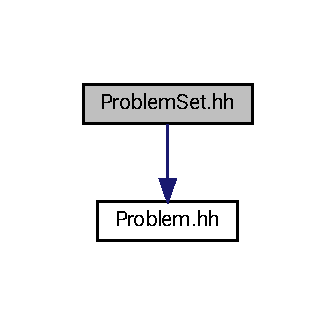
\includegraphics[width=161pt]{_problem_set_8hh__incl}
\end{center}
\end{figure}
\subsection*{Clases}
\begin{DoxyCompactItemize}
\item 
class \mbox{\hyperlink{class_problem_set}{Problem\+Set}}
\begin{DoxyCompactList}\small\item\em Representa un conjunto de problemas ordenados por id. \end{DoxyCompactList}\end{DoxyCompactItemize}


\subsection{Descripción detallada}
Especificación de la clase \mbox{\hyperlink{class_problem_set}{Problem\+Set}}. 


\hypertarget{_sesion_8hh}{}\section{Referencia del Archivo Sesion.\+hh}
\label{_sesion_8hh}\index{Sesion.\+hh@{Sesion.\+hh}}


Especificación de la clase \mbox{\hyperlink{class_sesion}{Sesion}}.  


\subsection*{Clases}
\begin{DoxyCompactItemize}
\item 
class \mbox{\hyperlink{class_sesion}{Sesion}}
\begin{DoxyCompactList}\small\item\em Representa una sesion con el numero de problemas en esta contenidos en un \mbox{\hyperlink{class_bin_tree}{Bin\+Tree}}. \end{DoxyCompactList}\end{DoxyCompactItemize}


\subsection{Descripción detallada}
Especificación de la clase \mbox{\hyperlink{class_sesion}{Sesion}}. 


\hypertarget{_sesion_set_8hh}{}\section{Referencia del Archivo Sesion\+Set.\+hh}
\label{_sesion_set_8hh}\index{Sesion\+Set.\+hh@{Sesion\+Set.\+hh}}


Especificación de la clase \mbox{\hyperlink{class_sesion_set}{Sesion\+Set}}.  


Dependencia gráfica adjunta para Sesion\+Set.\+hh\+:\nopagebreak
\begin{figure}[H]
\begin{center}
\leavevmode
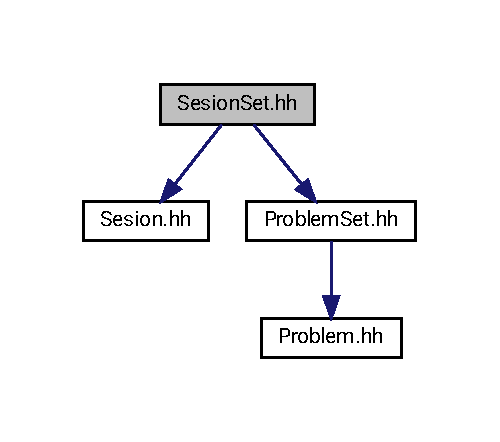
\includegraphics[width=240pt]{_sesion_set_8hh__incl}
\end{center}
\end{figure}
\subsection*{Clases}
\begin{DoxyCompactItemize}
\item 
class \mbox{\hyperlink{class_sesion_set}{Sesion\+Set}}
\begin{DoxyCompactList}\small\item\em Representa un conjunto de sesiones ordenados por id. \end{DoxyCompactList}\end{DoxyCompactItemize}


\subsection{Descripción detallada}
Especificación de la clase \mbox{\hyperlink{class_sesion_set}{Sesion\+Set}}. 


\hypertarget{_user_8hh}{}\section{Referencia del Archivo User.\+hh}
\label{_user_8hh}\index{User.\+hh@{User.\+hh}}


Especificación de la clase Usuario.  


Dependencia gráfica adjunta para User.\+hh\+:\nopagebreak
\begin{figure}[H]
\begin{center}
\leavevmode
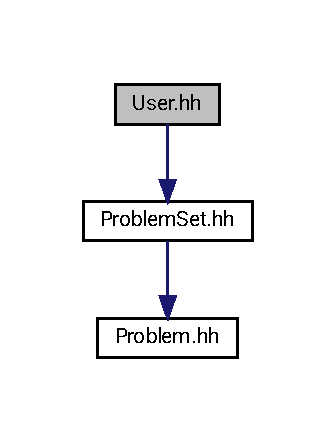
\includegraphics[width=161pt]{_user_8hh__incl}
\end{center}
\end{figure}
\subsection*{Clases}
\begin{DoxyCompactItemize}
\item 
class \mbox{\hyperlink{class_user}{User}}
\begin{DoxyCompactList}\small\item\em Representa un usuario con el numero de envios\+\_\+totales que ha realizado, el número de problemas resueltos, el número de problemas intentados en total, el curso en el qual está inscrito (si lo está) y dos \mbox{\hyperlink{class_problem_set}{Problem\+Set}} con los problemas\+\_\+resueltos y los problemas\+\_\+enviables respectivamente. \end{DoxyCompactList}\end{DoxyCompactItemize}


\subsection{Descripción detallada}
Especificación de la clase Usuario. 


\hypertarget{_user_set_8hh}{}\section{Referencia del Archivo User\+Set.\+hh}
\label{_user_set_8hh}\index{User\+Set.\+hh@{User\+Set.\+hh}}


Especificación de la clase \mbox{\hyperlink{class_user_set}{User\+Set}}.  


Dependencia gráfica adjunta para User\+Set.\+hh\+:\nopagebreak
\begin{figure}[H]
\begin{center}
\leavevmode
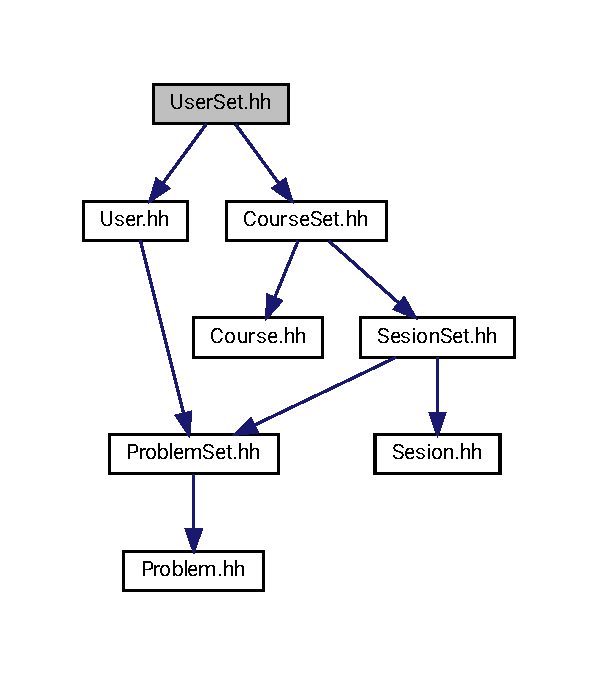
\includegraphics[width=287pt]{_user_set_8hh__incl}
\end{center}
\end{figure}
\subsection*{Clases}
\begin{DoxyCompactItemize}
\item 
class \mbox{\hyperlink{class_user_set}{User\+Set}}
\begin{DoxyCompactList}\small\item\em Representa un conjunto de usuario ordenados crecientemente por id. \end{DoxyCompactList}\end{DoxyCompactItemize}


\subsection{Descripción detallada}
Especificación de la clase \mbox{\hyperlink{class_user_set}{User\+Set}}. 


%--- End generated contents ---

% Index
\backmatter
\newpage
\phantomsection
\clearemptydoublepage
\addcontentsline{toc}{chapter}{Índice}
\printindex

\end{document}
